% Algorithmique I à la HEB-ESI
% ----------------------------------
\documentclass[a4paper,oneside]{book}

% Les styles
% ----------------------------------
% ===============================================================
% Feuille de style LaTeX pour le cours d'algorithmique 1ère à l'ESI
% ===============================================================

% ===================================================
%   Les gros éléments de mise en page
% ===================================================

% Spécifie que les fichiers sources sont codés en UTF8
% http://www.ctan.org/pkg/inputenc
% ----------------------------------------------------
\usepackage[utf8]{inputenc}

% Francisation des textes
% http://en.wikibooks.org/wiki/LaTeX/Internationalization#Babel
% -------------------------------------------------------------
\usepackage[francais]{babel}
\usepackage[T1]{fontenc}		% Permet de taper des accents

% Plus belles polices vectorielles que computer roman
% http://www.tug.dk/FontCatalogue/lmodern/
% -------------------------------------------------------------
\usepackage{lmodern}			

% Régler les marges des pages
% http://www.ctan.org/pkg/geometry
% vmargin: 1cm de plus automatique
% -------------------------------------------------------------
\usepackage[lmargin=3.5cm,rmargin=3.5cm,vmargin=3cm,footskip=4\baselineskip]{geometry}

% Enlever l'indentation de chaque première ligne de paragraphe
% + léger espace entre les paragraphes.
% http://www.ctan.org/pkg/parskip
% -------------------------------------------------------------
\usepackage{parskip}

% Permet d'avoir des couleurs
% usenames et dvipsnames pour noms prédéfinis
% http://www.ctan.org/pkg/xcolor
% -------------------------------------------------------------
\usepackage[usenames,dvipsnames,svgnames,table]{xcolor}

% Permet de barrer, souligner, ...
% Pour barrer : \sout{texte}
% -------------------------------------------------------------
\usepackage[normalem]{ulem}

% Gestion des images.
% http://www.ctan.org/pkg/graphicx
% -------------------------------------------------------------
\usepackage{graphicx}

% Pour disposer du symbole Euro
% -------------------------------------------------------------
\usepackage[official]{eurosym}

% subscript facile
% -------------------------------------------------------------
\newcommand\textsubscript[1]{\ensuremath{{}_{\mathrm{#1}}}}

% Hyperliens et URL
% http://www.ctan.org/pkg/hyperref
% -------------------------------------------------------------
\usepackage{hyperref}
\hypersetup{
  colorlinks = true,  % Colours links instead of ugly boxes
  urlcolor   = blue,  % Colour for external hyperlinks
  linkcolor  = black  % Colour of internal links
}

% Permet d'avoir les numéros de (sub)sections dans la marge
% Tiré de "Latex Howtos" de Sébastien Combéfis
% -------------------------------------------------------------
\makeatletter
\def\@seccntformat#1{\protect\makebox[0pt][r]{\csname the#1\endcsname\quad}}
\makeatother

% Framed permet d'avoir du texte avec une barre à gauche
%\usepackage{framed}
%\colorlet{shadecolor}{gray!50}
%\renewenvironment{leftbar}{%
  %\def\FrameCommand{\textcolor{shadecolor}{\vrule width 1pt} \hspace{10pt}}%
  %\MakeFramed {\advance\hsize-\width \FrameRestore}}%
%{\endMakeFramed}

% Modification du style pour les captions des figures
\usepackage[font=scriptsize,labelfont=sc,position=below]{caption}

% Plus d'options pour les notes/icones en marge
\usepackage{marginnote}
\reversemarginpar

% Pour un plus beau style pour le titre de chapitre
\usepackage[Lenny]{fncychap}

% Pour avoir Ovalbox
\usepackage{fancybox}

% Un grand contrôle sur l'aspect des listes
% Note: bizarrement, \setlist ne fonctionne pas (\itemize avec options non plus) 
% (clash avec un autre package ?)
% -------------------------------------------------------------
\usepackage{enumitem}
\setdescription{font=\sffamily\bfseries, style=nextline, leftmargin=*}
% Environnement liste, alternative à itemize, plus aéré.
\newlist{liste}{itemize}{3}
\setlist[liste]{label=$\triangleright$,leftmargin=8mm,itemsep=1mm}

% Permet d'avoir des références plus lisibles 
% ex: cf. figure 1 page suivante.
% http://www.ctan.org/pkg/varioref
% -------------------------------------------------------------
\usepackage[french]{varioref}

% Gestion de l'entête et du pied de page
% http://www.ctan.org/pkg/fancyhdr
% -------------------------------------------------------------
\usepackage{fancyhdr}
\setlength{\headheight}{13pt} 
\fancyhf{} % Enlever tout
\renewcommand{\headrulewidth}{0pt} % pas de ligne en entête
\fancyfoot[C]{\textcolor{gray}{---\ \thepage\ ---}}
\fancyhead[R]{\ifnum\value{chapter}>0 \textcolor{gray}{\up{\leftmark}} \fi}
\fancypagestyle{plain}{				% Redéfinir le style plain
	\fancyhf{} 						% Enlever tout
	\fancyfoot[C]{\textcolor{gray}{---\ \thepage\ ---}}
	\renewcommand{\headrulewidth}{0pt} % pas de ligne en entête
}


% ===================================================
%   Commandes et environnements
% ===================================================

% Met en évidence un ou des paragraphes
% titre en gras encadré + croix
% cf. http://tex.stackexchange.com/questions/33078/frame-with-only-crosses-in-two-opposite-corners
\newenvironment{Emphase}[2][]{%
	\section*{\ifthenelse{\not\equal{#1}{}}{\marginnote{\includegraphics[width=25px]{icon/#1}}[2pt]}{}\ovalbox{\normalsize\textbf{#2}}}
	\vspace{-10mm}
	{\color{gray}\par\hfill\rlap{\kern-0.5cm\rule{1cm}{0.4pt}\kern-0.2cm\rule[-0.8cm]{0.4pt}{1cm}}}%
    \vskip-\baselineskip
}{
	{\color{gray}\par\kern-0.8cm\hskip-0.25cm\rule{0.4pt}{1cm}\kern-0.2cm\rule[0.2cm]{1cm}{0.4pt}\par}
	\smallskip
}

% Pour mettre une icone en marge
% Utilisation: \marginicon{nomIcone}
% L'icone doit être présente dans le dossier icon
% dans un format reconnu (pas de gif)
\newcommand{\marginicon}[1]{
	\marginnote{\includegraphics[width=25px]{icon/#1}}[8pt]
}

% Affiche un cadre ovale coloré autour de texte, coloré aussi et en sansserif.
% Pour encadré numéro d'exercice, de tutoriel, ....
% -------------------------------------------------------------
\newcommand{\Cadre}[1]{{\sffamily\Ovalbox{#1}}}

% Pour un exercice avec numérotation automatique
\newcounter{exercicenum}[chapter]
\setcounter{exercicenum}{0}
\newenvironment{Exercice}[1]{%
	\refstepcounter{exercicenum}%
	%\renewcommand{\Currentlabel}{\arabic{chapter}.\theexercicenum}% Pour référence dans la solution
	\vspace{-2mm}
	\subsection*{\normalsize{\color{MidnightBlue}\Cadre{\theexercicenum}}\quad{\sffamily\bfseries#1}}
	\vspace{-2mm}
	}{%
	}
	
% Citation en début de chapitre
\newenvironment{Exergue}{%
	\begin{quote}
	\itshape
	}{
	\end{quote}
	\vskip2\baselineskip
	}

% Permet d'avoir plusieurs colonnes
% Utilisé dans les tableaux pour avoir un contrôle fin des |
\usepackage{multicol}

% Pour les tableaux
% ------------------
\usepackage{hhline} % Permet une gestion fine des barres horizontales 
% Aucune udée de l'intérêt pour les 3 lignes suivantes
\makeatletter
\newcommand\arraybslash{\let\\\@arraycr}
\makeatother{}
\setlength\tabcolsep{1mm} % aére le texte dans les cases de tableau
      % Style principal pour le bouquin
% Adaptation du package algorithmicx pour écrire les algorithmes
% du cours de logique à l'ESI

\usepackage{algpseudocode}		% Perme d'écrire des algorithmes
%\usepackage{algorithm}			% Pour des algorithmes flottants

% ==============================================================
% pseudocode et Pseudocode
% ==============================================================

\newenvironment{pseudo}{%
	\begin{minipage}{0.95\linewidth}
	\begin{sffamily}
	\begin{algorithmic}[0]
	\small
}{%
	\end{algorithmic}
	\end{sffamily}
	\end{minipage}
}
\newcommand{\cadre}[1]{%
	\fcolorbox{gray}{gray!10}{%
		\begin{minipage}{0.97\linewidth}#1\end{minipage}%
	}%
	\smallskip
}
\usepackage{environ} % Merci à astalavista pour ce truc :)
\NewEnviron{Pseudocode}{%
	\cadre{
		\begin{pseudo}
			\BODY
		\end{pseudo}
	}
}
\newcommand{\pseudocode}{\textsf}

% ==============================================================================
% Le code suivant permet d'avoir des lignes verticales pour délimiter les blocs. 
% cf: http://tex.stackexchange.com/questions/52473/is-it-possible-to-have-connecting-loop-lines-like-algorithm2e-in-algorithmic
% J'ai changé la ligne (plus grosse et grise)
% ==============================================================================

% --- Définitions techniques pour avoir les lignes
\makeatletter
\definecolor{rulecolor}{gray}{0.7} % This is the vertical rule that is inserted
\def\therule{\makebox[\algorithmicindent][l]{\hspace*{.4em}{\color{rulecolor}\vrule height .75\baselineskip width 0.05em depth .25\baselineskip}}}%

\newtoks\therules% Contains rules
\therules={}% Start with empty token list
\def\appendto#1#2{\expandafter#1\expandafter{\the#1#2}}% Append to token list
\def\gobblefirst#1{% Remove (first) from token list
  #1\expandafter\expandafter\expandafter{\expandafter\@gobble\the#1}}%
\def\LState{\State\unskip\the\therules}% New line-state
\def\pushindent{\appendto\therules\therule}%
\def\popindent{\gobblefirst\therules}%
\def\printindent{\unskip\the\therules}%
\def\printandpush{\printindent\pushindent}%
\def\popandprint{\popindent\printindent}%

% --- Définition des structures qui vont avoir une ligne
% Boucles
\algdef{SE}[WHILE]{While}{EndWhile}[1]
  {\printandpush\algorithmicwhile\ #1\ \algorithmicdo}
  {\popandprint\algorithmicend\ \algorithmicwhile}%
\algdef{SE}[FOR]{For}{EndFor}[1]
  {\printandpush\algorithmicfor\ #1\ \algorithmicdo}
  {\popandprint\algorithmicend\ \algorithmicfor}%
\algdef{SE}[REPEAT]{Repeat}{Until}
  {\printandpush\algorithmicrepeat}[1]
  {\popandprint\algorithmicuntil\ #1}%
% Alternatives
\algdef{SE}[IF]{If}{EndIf}[1]
  {\printandpush\algorithmicif\ #1\ \algorithmicthen}
  {\popandprint\algorithmicend\ \algorithmicif}%
\algdef{C}[IF]{IF}{ElsIf}[1]
  {\popandprint\pushindent\algorithmicelse\ \algorithmicif\ #1\ \algorithmicthen}%
\algdef{Ce}[ELSE]{IF}{Else}{EndIf}
  {\popandprint\pushindent\algorithmicelse}%
\algdef{SE}[SWITCH]{Switch}{EndSwitch}[1]
  {\printandpush\algorithmicswitch\ #1}
  {\popandprint\algorithmicend\ \algorithmicswitch}%
\algdef{C}[SWITCH]{SWITCH}{Case}[1]
  {\popandprint\pushindent\ #1:}%
% Structures
\algdef{SE}[STRUCT]{Struct}{EndStruct}[1]
  {\printandpush\algorithmicstruct\ #1}
  {\popandprint\algorithmicend\ \algorithmicstruct}%
% Classe
\algdef{SE}[CLASS]{Class}{EndClass}[1]
  {\printandpush\algorithmicclass\ #1}
  {\popandprint\algorithmicend\ \algorithmicclass}%
% Bloc customisable
\algdef{SE}[CUSTOM]{Custom}{EndCustom}
  {\printandpush}
  {\popandprint}
% Bloc
\algdef{SE}[BLOC]{Block}{EndBlock}[1]
  {\printandpush \algorithmicblock\ #1}
  {\popandprint \algorithmicend\ \algorithmicblock}
% Module
\algblockdefx[MODULE]{Module}{EndModule}[3]%
  {\printandpush\algorithmicprocedure\ \textproc{#1}(#2)\ifthenelse{\equal{#3}{}}{}{\Gives\ #3}}
  {\popandprint\algorithmicend\ \algorithmicprocedure}
% Méthode
\algblockdefx[METHOD]{Method}{EndMethod}[3]%
  {\printandpush\algorithmicmethod\ \textproc{#1}(#2)\ifthenelse{\equal{#3}{}}{}{\Gives\ #3}}
  {\popandprint\algorithmicend\ \algorithmicmethod}
% Constructeur
\algblockdefx[CONSTR]{Constr}{EndConstr}[2]%
  {\printandpush\algorithmicconstr\ \textproc{#1}(#2)}
  {\popandprint\algorithmicend\ \algorithmicconstr}
% Parties privées/publiques
\algdef{C}[CLASS]{CLASS}{Private}{\popandprint\pushindent\ privé:}%
\algdef{C}[CLASS]{CLASS}{Public}{\popandprint\pushindent\ public:}%
% Signatures de module / méthode / constructeur
\newcommand{\ModuleSign}[3]{\Stmt \algorithmicprocedure\ \textproc{#1}(#2)\ifthenelse{\equal{#3}{}}{}{\Gives\ #3}}
\newcommand{\MethodSign}[3]{\Stmt \algorithmicmethod\ \textproc{#1}(#2)\ifthenelse{\equal{#3}{}}{}{\Gives\ #3}}
\newcommand{\ConstrSign}[2]{\Stmt \algorithmicconstr\ \textproc{#1}(#2)}
  
% ==============================================================================
% Ajouts propres pour la francisation des termes prédéfinis + nouveaux termes
% ==============================================================================
\algnewcommand\algorithmicclass{\textbf{classe}}
\algnewcommand\algorithmicmethod{\textbf{méthode}}
\algnewcommand\algorithmicconstr{\textbf{constructeur}}
\algnewcommand\algorithmicstruct{\textbf{structure}}
\algnewcommand\algorithmicblock{\textbf{bloc}}
\algnewcommand\algorithmicbegin{\textbf{début}}
\algrenewcommand\algorithmicend{\textbf{fin}}
\algrenewcommand\algorithmicprocedure{\textbf{module}}
\algrenewcommand\algorithmicfunction{\textbf{module}}
\algrenewcommand\algorithmicwhile{\textbf{tant que}}
\algrenewcommand\algorithmicfor{\textbf{pour}}
\algrenewcommand\algorithmicrepeat{\textbf{faire}}
\algrenewcommand\algorithmicuntil{\textbf{jusqu'à ce que}}
\algrenewcommand\algorithmicdo{\textbf{faire}}
\algrenewcommand\algorithmicreturn{\textbf{retourner}}
\algrenewcommand\algorithmicif{\textbf{si}}
\algrenewcommand\algorithmicthen{\textbf{alors}}
\algrenewcommand\algorithmicelse{\textbf{sinon}}
\algnewcommand\algorithmicswitch{\textbf{selon que}}

% ==============================================================================
% Ajout de petits éléments de syntaxe non existants
% ==============================================================================
\newcommand{\In}{\ensuremath{\downarrow}}
\newcommand{\Out}{\ensuremath{\uparrow}}
\newcommand{\InOut}{\In{}\Out{}}
\newcommand{\Gets}{\ensuremath{\gets}\ }
\newcommand{\Gives}{\ \ensuremath{\rightarrow}{}}
\newcommand{\K}[1]{\textbf{#1}} % Keyword
\newcommand{\Decl}{\LState}
\renewcommand{\Return}{\LState\algorithmicreturn\ }
\newcommand{\Open}{\LState\textbf{ouvrir}\ }
\newcommand{\Close}{\LState\textbf{fermer}\ }
\newcommand{\Read}{\LState\textbf{lire}\ }
\newcommand{\Readf}{\LState\textbf{lire}\ }
\newcommand{\Write}{\LState\textbf{afficher}\ }
\newcommand{\Writef}{\LState\textbf{écrire}\ }
\newcommand{\Empty}{\LState}
\newcommand{\Stmt}{\LState}
\newcommand{\Let}{\LState}
\newcommand{\Error}{\LState\textbf{erreur}\ }
% Les commentaires
\algrenewcommand{\algorithmiccomment}[1]{{\small\hskip1em// #1}}
\newcommand{\LComment}{\Empty\hskip-1em\Comment}
\newcommand{\RComment}{\hfill\Comment}
% Pour indenter une ligne
\newcommand{\Indent}{\expandafter\hskip\algorithmicindent\relax}
% Pour une continuation de ligne (2x indenté)
\newcommand{\Suite}{\Stmt\Indent\Indent}

% ==============================================================================
% Modifications de style
% ==============================================================================
\algrenewcommand\textproc{\textit} % Nom de module en italique plutôt qu'en small caps
   % Définition pour les algorithmes

% Identité de l'école
% ----------------------------------
\newcommand{\ecole}{Haute École de Bruxelles}
\newcommand{\entite}{École Supérieure d'Informatique}
\newcommand{\entiteadresse}{Rue Royale, 67 – 1000 Bruxelles}
\newcommand{\entitesite}{www.heb.be/esi}
\newcommand{\entitetel}{02/219.15.46}
\newcommand{\entitemail}{esi@heb.be}
\newcommand{\etude}{Bachelor en Informatique}

% Identité de l'AA
% ----------------------------------
\newcommand{\ue}{DEV1}
\newcommand{\cours}{Algorithmique I}

% Éléments temporels : année - prof
% ----------------------------------
\newcommand{\annee}{2014}
\newcommand{\auteura}{L. Beeckmans}
\newcommand{\auteurb}{M. Codutti}
\newcommand{\auteurc}{G. Cuvelier}
\newcommand{\auteurd}{J. Dossogne}
\newcommand{\auteure}{A. Hallal}
\newcommand{\auteurf}{C. Leruste}
\newcommand{\auteurg}{E. Levy}
\newcommand{\auteurh}{N. Pettiaux}
\newcommand{\auteuri}{F. Servais}
\newcommand{\auteurj}{W. Willame}
\newcommand{\contact}{mcodutti@heb.be}
\newcommand{\ladate}{\today}

% Index (attendre qu'il soit suffisament rempli)
% ----------------------------------
%\usepackage{makeidx} % pour générer un index
%\makeindex

% Les différentes parties du document
% -----------------------------------
\begin{document}
% =======================================================
% Syllabus de Logique 1ère - Début du document
% =======================================================

% =======================================================
% Page de garde
% =======================================================

\thispagestyle{empty}

% haut-gauche

\includegraphics[scale=0.45]{image/logo-esi}
\begin{minipage}[t]{7cm}
\vspace{-6.5\baselineskip}
\sffamily
\large\textbf{\ecole\\\entite}
\\\vspace{3.5mm}\\
\large\entiteadresse\\\entitetel{} – \entitemail
\end{minipage}
%
% haut-droit
\begin{minipage}[t]{5cm}
\vspace{-6.5\baselineskip}
\sffamily
\raggedleft
\large\textbf{\etude}
\end{minipage}


% centre
\vfill
\begin{center}
\sffamily
\Huge\cours
\bigskip\\
\Large\ue\ -- \annee
\end{center}
\vfill

%bas
Activité d'apprentissage enseignée par :
\begin{center}
\itshape 
\begin{tabular}{*{5}{p{2.2cm}}}
À définir\dots
%\auteura & \auteurb & \auteurc & \auteurd & \auteure \\
%\auteurf & \auteurg & \auteurh & \auteuri & \auteurj \\
\end{tabular}
\end{center}

% =======================================================
% 2ème page : licence, infos de version, ...
% =======================================================

\clearpage
\thispagestyle{empty}

\vfill

Ce syllabus a été écrit à l'origine par M. Monbaliu
à une époque où le cours s'appelait 
\og\ Logique et techniques de programmation \fg.
Il a ensuite été adapté par Mme~Leruste, M.~Beeckmans et M.~Codutti.
Qu'ils en soient tous remerciés.
Nous remercions également tous ceux qui ont contribué à son amélioration
grâce à leur lecture attentive et leurs remarques. 

\bigskip
Document produit avec \LaTeX.
\\Version du \today.

\vfill


\includegraphics[width=25mm]{image/cc-gris}
\\
Ce document est distribué sous licence 
\\Creative Commons Paternité - Partage à l'Identique 2.0 Belgique 
\\(http://creativecommons.org/licenses/by-sa/2.0/be/).
\\Les autorisations au-delà du champ de cette licence
\\peuvent être obtenues à \entitesite{} - \texttt{\contact}.
\pagestyle{fancy}

% =======================================================
% Table des matières
% =======================================================
\setcounter{tocdepth}{1}
\tableofcontents{}


% =====================================
\chapter{Qu’est-ce qu’un algorithme~?}
% =====================================

	\begin{Exergue}
		«~L’algorithmique est le permis de conduire de l’informatique.
		Sans elle, il n’est pas concevable d’exploiter sans risque un ordinateur.~»
		\footnote{[CORMEN e.a., Algorithmique, Paris, Edit. Dunod, 2010, (Cours, 
		exercices et problèmes), p. V] }
	\end{Exergue}

	\marginicon{objectif}
	Ce chapitre a pour but de vous faire comprendre ce
	qu’est un \textbf{algorithme} et à quel moment de
	l’\textbf{activité de programmation} il intervient. 
	Nous tenterons de préciser la différence entre un algorithme 
	et un \textbf{programme}.
	
	Il situe, enfin, le cours d'algorithmique
	dans l’ensemble des cours donnés dans le baccalauréat et
	en trace les lignes principales.

\section{La notion de problème}

	\subsection{Préliminaires~:~utilité de l’ordinateur}
	
		L’ordinateur est une machine. Mais une machine intéressante dans la
		mesure où elle est destinée d’une part, à nous décharger d’une
		multitude de tâches peu valorisantes, rébarbatives telles que le
		travail administratif répétitif, mais surtout parce qu’elle est capable
		de nous aider, voire nous remplacer, dans des tâches plus ardues qu’il
		nous serait impossible de résoudre sans son existence (conquête
		spatiale, prévision météorologique, jeux vidéo, \dots).
		
		En première approche, nous pourrions dire que l’ordinateur est destiné à
		nous remplacer, à faire à notre place (plus rapidement et probablement
		avec moins d’erreurs) un travail nécessaire à la résolution de
		\textbf{problèmes} auxquels nous devons faire face. Attention~! Il
		s’agit bien de résoudre des \textit{problèmes} et non des mystères
		(celui de l’existence, par exemple). Il faut que la question à laquelle
		on souhaite répondre soit \textbf{accessible à la raison}.

	\subsection{Poser le problème \index{Poser le probleme@Poser le problème}}
	
		Un préalable à l’activité de résolution d’un problème est bien de
		\textbf{définir} d’abord quel est le problème posé, en quoi il consiste
		exactement ; par exemple, faire un baba au rhum, réussir une année
		d’études, résoudre une équation mathématique\dots
		
		Un problème bien posé doit mentionner l’\textbf{objectif à atteindre},
		c’est-à-dire la situation d’arrivée, le but escompté, le résultat
		attendu. Généralement, tout problème se définit d’abord explicitement
		par ce que l’on souhaite obtenir.
		
		La formulation d’un problème ne serait pas complète sans la connaissance
		des \textbf{données du problème} et \textbf{du cadre dans lequel se
		pose le problème~:}~de quoi dispose-t-on, quelles sont les hypothèses
		de base, quelle est la situation de départ~? Faire un baba au rhum est
		un problème tout à fait différent s’il faut le faire en plein désert ou
		dans une cuisine super équipée~! D’ailleurs, dans certains cas, la
		première phase de la résolution d’un problème consiste à mettre à sa
		disposition les éléments nécessaires à sa résolution~:~dans notre
		exemple, ce serait se procurer les ingrédients et les ustensiles de
		cuisine.
	
		Un problème ne sera véritablement bien spécifié que s’il s’inscrit dans
		le schéma suivant~:
		
		% Voir si j’en fais un environnement.
		\begin{center}
		\begin{Ovalbox}
		{\textbf{étant donné} [les données] \textbf{on demande} [l’objectif]}
		\end{Ovalbox}
		\end{center}
	
		Parfois, la première étape dans la résolution d’un problème est de
		préciser ce problème à partir d’un énoncé flou~:~il ne s’agit pas
		nécessairement d’un travail facile~!

		\begin{Emphase}[exercice]{Exercice~:~Un problème flou}
			Soit le problème suivant~:~«~Calculer la moyenne de nombres entiers.~».
			\\Qu’est-ce qui vous parait flou dans cet énoncé~?
		\end{Emphase}

		Une fois le problème correctement posé, on passe à la recherche et la
		description d’une \textbf{méthode de résolution}, afin de savoir
		comment faire pour atteindre l’objectif demandé à partir de ce qui est
		donné. Le \textbf{nom} donné à une méthode de résolution varie en
		fonction du cadre dans lequel se pose le problème~:~\textit{façon de
		procéder, mode d’emploi, marche à suivre, guide, patron, modèle,
		recette de cuisine, méthode ou plan de travail, algorithme
		mathématique, programme, directives d’utilisation, \dots}

\section{Procédure de résolution\index{Procedure de resolution@Procédure de
résolution}}

	Une \textbf{procédure de résolution} est une description en termes
	compréhensibles par l’exécutant de la \textbf{marche à
	suivre} pour résoudre un problème donné.
	
	On trouve beaucoup d’exemples dans la vie courante~:
	recette de cuisine, mode d’emploi d’un GSM, description d’un
	itinéraire, plan de montage d’un jeu de construction, etc. Il est clair
	qu’il y a une infinité de rédactions possibles de ces différentes
	marches à suivre. Certaines pourraient être plus précises que d’autres,
	d’autres par contre pourraient s’avérer exagérément explicatives.
	
	Des différents exemples de procédures de résolution se dégagent les
	caractéristiques suivantes~:

	\begin{liste}
	\item toutes ont un \textbf{nom}
	\item elles s’expriment dans un \textbf{langage}
		(français, anglais, dessins\dots)
	\item l’ensemble de la procédure consiste 
		en une \textbf{série chronologique}
		d’instructions ou de phrases (parfois numérotées)
	\item une instruction se caractérise par un ordre, 
		une action à accomplir,
		une \textbf{opération} à exécuter sur les \textbf{données} du problème
	\item certaines phrases justifient ou expliquent ce qui se passe~:~
		ce sont des \textbf{commentaires}.
	\end{liste}

	On pourra donc définir, en première approche, une procédure de
	résolution comme un texte, écrit dans un certain langage, qui décrit
	une suite d’actions à exécuter dans un ordre précis, ces actions
	opérant sur des objets issus des données du problème.

	\subsection{Chronologie des opérations}

		Pour ce qui concerne l’ordinateur, le travail d’exécution d’une marche à
		suivre est impérativement \textbf{séquentiel}. C’est-à-dire que les
		instructions d’une procédure de résolution sont exécutées \textbf{une
		et une seule fois} dans l’ordre où elles apparaissent dans le code.
		Cependant certains artifices d’écriture permettent de \textbf{répéter}
		l’exécution d’opérations ou de la \textbf{conditionner}
		(c’est-à-dire de choisir si
		l’exécution aura lieu oui ou non en fonction de la
		réalisation d’une condition).

	\subsection{Les opérations élémentaires}


		Dans la description d’une marche à suivre, la plupart des opérations
		sont introduites par un \textbf{verbe
		}(\textit{remplir}, \textit{verser, prendre, peler},
		etc.). L’exécutant ne pourra exécuter une action que s’il la comprend~:
		cette action doit, pour lui, être une action élémentaire, une action
		qu’il peut réaliser sans qu’on ne doive lui donner des explications
		complémentaires. Ce genre d’opération élémentaire est appelée
		\textbf{primitive}.
		
		Ce concept est évidement relatif à ce qu’un exécutant est capable de
		réaliser. Cette capacité, il la possède d’abord parce qu’il est
		\textbf{construit} d’une certaine façon (capacité innée). Ensuite parce
		que, par construction aussi, il est doté d’une faculté
		d’\textbf{apprentissage} lui permettant d’assimiler, petit à petit, des
		procédures non élémentaires qu’il exécute souvent. Une opération non
		élémentaire pourra devenir une primitive un peu plus tard.
		
	\subsection{Les opérations bien définies}

		Il arrive de trouver dans certaines marches à suivre des opérations qui
		peuvent dépendre d’une certaine manière de l’appréciation de
		l’exécutant. Par exemple, dans une recette de cuisine on pourrait 
		lire~:~\textit{ajouter} \textbf{\textit{une pincée}} \textit{de vinaigre,
		saler et poivrer} \textbf{\textit{à volonté}}, \textit{laisser cuire
		une} \textbf{\textit{bonne}}\textit{ heure dans un four
		}\textbf{\textit{bien}} \textit{chaud, etc.}
		
		Des instructions floues de ce genre sont dangereuses à faire figurer
		dans une bonne marche à suivre car elles font appel à une appréciation
		arbitraire de l’exécutant. Le résultat obtenu risque
		d’être imprévisible d’une exécution à l’autre. De plus, les termes du
		type \textit{environ, beaucoup, pas trop} et \textit{à peu près} sont
		intraduisibles et proscrites au niveau d’un langage informatique~!
		\footnote{Le lecteur intéressé découvrira dans la littérature
		spécialisée que même les procédures de génération de nombres aléatoires
		sont elles aussi issues d’algorithmes mathématiques tout à fait
		déterminés.}
		
		Une \textbf{opération bien définie} est donc une opération débarrassée
		de tout vocabulaire flou et dont le résultat est \textbf{entièrement
		prévisible}. Des versions «~bien définies~» des exemples ci-dessus
		pourraient être~:~\textit{ajouter 2~cl de vinaigre, ajouter 5~g de sel
		et 1~g de poivre, laisser cuire 65~minutes dans un four chauffé à
		220\degre, etc.}

		Afin de mettre en évidence la difficulté d’écrire une
		marche à suivre claire et non ambigüe, on vous propose
		l’expérience suivant.

\clearpage
		\begin{Emphase}[exercice]{Expérience~:~Le dessin}

			Cette expérience s’effectue en groupe.
			Le but est de faire un dessin et de permettre à une autre personne, qui
			ne l’a pas vu, de le reproduire fidèlement, au travers
			d’une «~marche à suivre~».

			\begin{enumerate}
			\item
				Chaque personne prend une feuille de papier et 
				y dessine quelque chose en quelques traits précis. 
				Le dessin ne doit pas être trop compliqué ; 
				on ne teste pas ici vos talents de dessinateur~! 
				(ça peut-être une maison, une voiture, \dots)
			\item
				Sur une \textbf{autre} feuille de papier, 
				chacun rédige des instructions permettant de 
				reproduire fidèlement son propre dessin. 
				Attention~! Il est important de ne
				\textbf{jamais faire référence à la signification du dessin}. 
				Ainsi, on peut écrire~:~«~dessine un rond~» 
				mais certainement pas~:~«~dessine une roue~».
			\item
				Chacun cache à présent son propre dessin et échange 
				sa feuille d’instructions avec celle de quelqu’un d’autre.
			\item
				Chacun s’efforce ensuite de reproduire le dessin d’un autre 
				en suivant \textbf{scrupuleusement} les instructions indiquées 
				sur la feuille reçue en échange, \textbf{sans tenter
				d’initiative} (par exemple en croyant avoir compris ce
				qu’il faut dessiner).
			\item
				Nous examinerons enfin les différences entre l’original et 
				la reproduction et nous tenterons de comprendre pourquoi 
				elles se sont produites (par imprécision des instructions ou
				par mauvaise interprétation de celles-ci par le dessinateur\dots)
			\end{enumerate}

		\end{Emphase}

\bigskip
		\marginicon{reflexion}
		Quelles réflexions cette expérience vous inspire-t-elle~?
		Quelle analogie voyez-vous avec une marche à suivre donnée à un
		ordinateur~?

		Dans cette expérience, nous imposons que la «~marche à suivre~» ne mentionne
		aucun mot expliquant le sens du dessin (mettre «~rond~» et pas «~roue~»
		par exemple). Pourquoi, à votre avis, avons-nous imposé cette
		contrainte~?

	\subsection{Opérations soumises à une condition}

		En français, l’utilisation de conjonctions ou locutions conjonctives du
		type \textit{si}, \textit{selon que}, \textit{au cas où}, \dots
		présuppose la possibilité de ne pas exécuter certaines opérations en
		fonction de certains événements. D’une exécution à l’autre de
		l’entièreté de la procédure, certaines de ses parties seront ou non
		exécutées.
		
		\textbf{Exemple~:}~Si la viande est surgelée, la décongeler à
		l’aide du four à micro-ondes.

	\subsection{Opérations à répéter}

		De la même manière, il est possible d’exprimer en français une exécution
		répétitive d’opérations en utilisant les mots \textit{tous},
		\textit{chaque}, \textit{tant que}, \textit{jusqu’à ce que},
		\textit{chaque fois que}, \textit{aussi longtemps que}, 
		\textit{faire x fois}, \dots 
		
		Dans certains cas, le nombre de répétitions est connu à l’avance
		(\textit{répéter 10 fois}) ou déterminé par une durée (\textit{faire
		cuire pendant 30 minutes}) et dans d’autres cas il est inconnu.
		Dans ce cas, la fin de la période
		de répétition d’un bloc d’opérations dépend alors de la réalisation
		d’une condition ((\textit{lancer le dé jusqu’à ce
		qu’il tombe sur 6}), \dots, \textit{faire cuire
		jusqu’à évaporation complète}\dots). C’est ici que réside le danger de
		boucle infinie, due à une mauvaise formulation de la condition d’arrêt.
		Par exemple~:~\textit{lancer le dé jusqu’à ce que le point 
		obtenu soit 7}\dots Bien sûr, un humain doté d’intelligence 
		comprend que la condition est impossible à réaliser, mais un robot 
		appliquant cette directive à la lettre lancera le dé 
		perpétuellement\dots

	\subsection{À propos des données}

		Les types d’objets figurant dans les diverses procédures de résolution
		sont fonction du cadre dans lequel s’inscrivent ces procédures, du
		domaine d’application de ces marches à suivre. Par exemple, pour une
		recette de cuisine, ce sont les ingrédients. Pour un jeu de
		construction ce sont les briques.
		
		L’ordinateur, quant à lui, manipule principalement
		des données numériques et textuelles. 
		Nous verrons plus tard comment on
		peut combiner ces données élémentaires pour obtenir 
		des données plus complexes.

\section{Algorithmes informatiques}

	Notre but étant de faire de l’informatique, il convient de restreindre
	notre étude à des notions plus précises, plus spécialisées, gravitant
	autour de la notion de \textit{traitement automatique de
	l’information}.

	\subsection{Algorithme}

		Un algorithme appartient au vaste ensemble des \textit{marches à
		suivre}.

		\marginicon{definition}
		\textbf{Algorithme}~:~Procédure de résolution d’un problème 
		ou d’un ensemble de problèmes de même type contenant des opérations
		bien définies portant sur des informations, s’exprimant dans une
		séquence définie sans ambigüité, destinée à être traduite dans 
		un langage de programmation.
	
		Comme toute marche à suivre, un algorithme doit s’exprimer dans un
		certain langage~:~à priori le langage naturel, mais il y a d’autres
		possibilités~:~ordinogramme, arbre programmatique, pseudo-code ou LDA
		(langage de description d’algorithmes) que nous allons utiliser dans le
		cadre de ce cours.

	\subsection{Programme}

		\marginicon{definition}
		Un \textbf{programme} n’est rien d’autre que la représentation d’un
		algorithme dans un langage plus technique compris par 
		un ordinateur (par exemple~:~Assembleur, Cobol, Java, 
		C++, \dots). Ce type de langage est appelé \textbf{langage de
		programmation}.
		
		Écrire un programme correct suppose donc la parfaite connaissance du
		langage de programmation et de sa \textbf{syntaxe}, qui est en quelque
		sorte la grammaire du langage. Mais ce n’est pas suffisant~! Puisque le
		programme est la représentation d’un algorithme, il faut que celui-ci
		soit correct pour que le programme le soit. Un programme correct
		résulte donc d’une démarche logique correcte (algorithme correct) et de
		la connaissance de la syntaxe d’un langage de programmation.
		
		Il est donc indispensable d’élaborer des algorithmes corrects avant
		d’espérer concevoir des programmes corrects.

	\subsection{Les constituants principaux de l’ordinateur}

		Les constituants d’un ordinateur se divisent en \textbf{hardware}
		(matériel) et \textbf{software d’exploitation} (logiciel).
		
		Le \textbf{hardware} est constitué de l’ordinateur proprement dit et
		regroupe les entités suivantes~:

		\begin{liste}
		\item
			\textbf{l’organe de contrôle~:}~c’est le cerveau de
			l’ordinateur. Il est l’organisateur, le contrôleur
			suprême de l’ensemble. Il assume l’enchainement des opérations
			élémentaires. Il s’occupe également d’organiser l’exécution effective
			de ces opérations élémentaires reprises dans les programmes.
		\item
			\textbf{l’organe de calcul~:}~c’est le calculateur où ont lieu les
			opérations arithmétiques ou logiques. Avec l’organe de contrôle, il
			constitue le \textbf{processeur} ou \textbf{unité centrale}.
		\item
			\textbf{la mémoire centrale~:}~dispositif permettant de mémoriser,
			pendant le temps nécessaire à l’exécution, les programmes et certaines
			données pour ces programmes.
		\item
			\textbf{les unités d’échange avec l’extérieur~:}’dispositifs permettant
			à l’ordinateur de recevoir des informations de l’extérieur (unités de
			lecture telles que clavier, souris, écran tactile, \dots) ou de
			communiquer des informations vers l’extérieur (unités d’écriture telles
			que écran, imprimantes, signaux sonores, \dots).
		\item
			\textbf{les unités de conservation à long terme~:}~ce sont les mémoires
			auxiliaires (disques durs, CD ou DVD de données, clés USB, \dots) sur
			lesquelles sont conservées les procédures (programmes) ou les
			informations résidentes dont le volume ou la fréquence d’utilisation ne
			justifient pas la conservation permanente en mémoire centrale.
		\end{liste}
		
		Le \textbf{software d’exploitation} est l’ensemble des procédures
		(programmes) s’occupant de la gestion du fonctionnement d’un système
		informatique et de la gestion de l’ensemble des ressources de ce
		système (le matériel –~les programmes~– les données). Il contient
		notamment des logiciels de traduction permettant d’obtenir un programme
		écrit en langage machine (langage technique qui est le seul que
		l’ordinateur peut comprendre directement, c’est-à-dire exécuter) à
		partir d’un programme écrit en langage de programmation plus ou moins
		«~évolué~» (c’est-à-dire plus ou moins proche du langage naturel).

	\subsection{Exécution d’un programme}

		Isolons (en les simplifiant) deux constituants essentiels de
		l’ordinateur afin de comprendre ce qui se passe quand
		un ordinateur exécute un programme. D’une part, la
		mémoire contient le programme et les données manipulées par ce
		programme. D’autre part, le processeur va «~exécuter~»
		ce programme.

		\begin{tabular}{m{0.46\linewidth}m{0.46\linewidth}}
			\begin{center}
			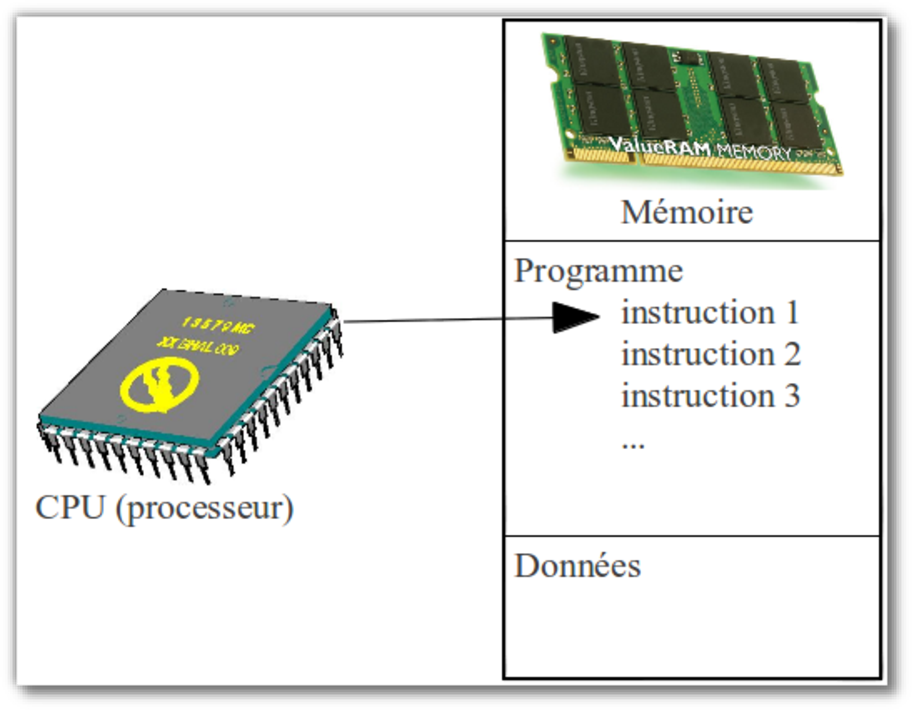
\includegraphics[width=0.45\textwidth]{image/intro-schema-ordi}
			\end{center}
		&
			\textbf{Comment fonctionne le processeur~?}
	
			De façon très simplifiée, on passe par les étapes suivantes~:
	
			\medskip
			\begin{flushleft}
			\begin{enumerate}
			\item Le processeur lit l’instruction courante.
			\item Il exécute cette instruction. Cela peut amener à manipuler les données.
			\item L’instruction suivante devient l’instruction courante.
			\item On revient au point 1.
			\end{enumerate}
			\end{flushleft}
		\\
		\end{tabular}

		On voit qu’il s’agit d’un travail
		automatique ne laissant aucune place à l’initiative~!

\section{Les phases d’élaboration d’un programme}

	Voyons pour résumer un schéma \textbf{simplifié} des phases par
	lesquelles il faut passer quand on développe un programme.

	\begin{tabular}{m{0.26\linewidth}m{0.68\linewidth}}
	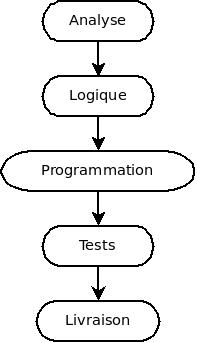
\includegraphics[width=3.5cm]{image/intro-phases-develop}
	&
	\begin{liste}
	\item 
		Lors de \textbf{l’analyse}, le problème doit être
		compris et clairement précisé. Vous aborderez cette phase dans le cours
		d’analyse.
	\item
		Une fois le problème analysé, et avant de passer à la phase de
		programmation, il faut réfléchir à l’\textbf{algorithme} qui va
		permettre de résoudre le problème. C’est à cette phase précise
		que s’attache ce cours.
	\item
		On peut alors \textbf{programmer} cet algorithme dans le langage de
		programmation choisi. Vos cours de langage (Java, Cobol, 
		Assembleur, \dots) sont dédiés à cette phase.
	\item
		Vient ensuite la phase de \textbf{tests} qui ne manquera pas de montrer
		qu’il subsiste des problèmes qu’il
		faut encore corriger. (Vous aurez maintes fois
		l’occasion de vous en rendre compte lors des
		séances de laboratoire)
	\item
		Le produit sans bug (connu) peut être \textbf{mis en application}
		ou \textbf{livré} à la personne qui vous en a passé la commande.
	\end{liste}
	\\
	\end{tabular}
	
	Notons que ce processus n’est pas linéaire. À chaque
	phase, on pourra détecter des erreurs, imprécisions ou oublis des
	phases précédentes et revenir en arrière.

	\textbf{Pourquoi passer par la phase «~logique~» 
		et ne pas directement passer à la programmation~?}
	
	Voilà une question que vous ne manquerez pas de vous poser pendant votre
	apprentissage cette année. Apportons quelques éléments de réflexion.

	\begin{liste}
	\item
		Passer par une phase de «~logique~» permet de séparer deux 
		difficultés~:~quelle est la marche à suivre~? Et comment l’exprimer
		dans le langage de programmation choisi~? Le langage que nous allons
		utiliser en logique est plus souple et plus général que le langage Java
		par exemple (où il faut être précis au «~;~» près).
	\item
		De plus, un algorithme écrit facilite le dialogue dans une équipe de
		développement. «~J’ai écrit un algorithme pour
		résoudre le problème qui nous occupe. Qu’en
		pensez-vous~? Pensez-vous qu’il est correct~?
		Avez-vous une meilleure idée~?~». L’algorithme est plus adapté à la
		communication car plus lisible.
	\item
		Enfin, si la logique est écrite, elle pourra facilement être traduite
		dans n’importe quel langage de programmation. La
		traduction d’un langage de programmation à un autre
		est un peu moins facile à cause des particularités propres à chaque
		langage.
	\end{liste}

	Bien sûr, cela n’a de sens que si le problème présente
	une réelle difficulté logique. Certains problèmes (en pratique,
	certaines parties de problèmes) sont suffisamment simples que pour être
	directement programmés. Mais qu’est-ce
	qu’un problème simple~? Cela va évidemment changer
	tout au long de votre apprentissage. Un problème qui vous paraitra
	difficile en début d’année vous paraitra (enfin, il
	faut l’espérer~!) une évidence en fin
	d’année.

\clearpage
\section{Une approche ludique de l'algorithmique}

	Il existe de nombreux programmes qui permettent de s'initier
	à la création d'algorithmes.
	Nous voudrions mettre en avant le projet \url{learn.code.org}.
	Soutenu par des grands noms de l'informatique comme 
	\textsf{Google}, \textsf{Microsoft}, \textsf{Facebook} et \textsf{Twitter}
	il permet de s'initier aux concepts de base
	(les boucles, les alternatives et la découpe en modules)
	au travers d'exercices ludiques faisant intervenir des
	personnages issus de jeux que les jeunes connaissent bien 
	(\textsf{Angry birds}, \textsf{Plantes et zombies}).
	
	Sur le site \url{learn.code.org} vous trouverez :
	\begin{liste}
	\item
		\og\ The Hour of Code\fg : 
		un survol des notions fondamentales en une heure
		au travers de vidéos explicatives
		et d'exercices interactifs.
	\item
		\og\ Intro aux cours d'informatique pour ado\fg : 
		un cours de 20 heures, 
		reprenant et approfondissant les éléments
		de \og\ The Hour of Code\fg.
	\end{liste}
	
	
\section{Conclusion}

	L’informatisation de problèmes est un processus essentiellement
	dynamique, contenant des allées-venues constantes entre les différentes
	étapes. Codifier un algorithme dans un langage de programmation
	quelconque n’est certainement pas la phase la plus difficile de ce
	processus. Par contre, élaborer une démarche logique de résolution d’un
	problème est probablement plus complexe.
	
	Le but du cours de \textbf{logique et techniques de programmation} est
	double~:

	\begin{liste}
	\item
		essayer de définir une bonne démarche d’élaboration d’algorithmes
		(apprentissage de la \textbf{logique} de programmation) ;
	\item
		faire comprendre l’intérêt d’utiliser certaines méthodes ou
		\textbf{techniques} classiques qui ont fait leurs preuves.
	\end{liste}

	Le tout devrait avoir pour résultat l’élaboration de \textit{bons
	programmes}, c’est-à-dire \textit{des programmes dont il est facile de
	se persuader qu’ils sont corrects} et des programmes dont la
	maintenance est la plus aisée possible. Dans ce sens, ce cours se situe
	idéalement en aval d’un cours d’\textbf{analyse}, et en amont des cours
	de \textbf{langage de programmation}. Ceux-ci sont idéalement complétés
	par les notions de \textbf{système d’exploitation} et de
	\textbf{fichiers}.

	Afin d’envisager la résolution d’une multiplicité de problèmes prenant
	leur source dans des domaines différents, le contenu minimum de ce
	cours envisage l’étude des points suivants (dans le désordre)~:

	\begin{liste}
	\item 
		la représentation des algorithmes
	\item
		la programmation structurée
	\item
		la programmation procédurale~:~les modules et 
		le passage de paramètres
	\item
		les bases de la programmation orientée objet
	\item
		la logique de traitement des fichiers séquentiels
	\item
		la logique de traitement des tableaux
	\item
		la résolution de problèmes récursifs
	\item
		la logique de traitement des structures de données particulières telles
		que listes, files d’attente, piles, arbres, graphes, tables de hachage,
		etc.
	\end{liste}

	Voilà bien un programme trop vaste pour un premier cours, 
	Un choix devra donc être fait et ce, en fonction
	de critères tels que la rapidité d’assimilation, l’intérêt des
	étudiants et les besoins exprimés pour des cours annexes. 
	Les matières non traitées ici, 
	le seront dans les cours d'Algorithmique II et III. 

% Supprimé tant qu'on n'a pas de référence plus récente, disponible en magasin.
%\section{Références}
	
	%Voici une liste de livres et sites que vous pouvez consulter
	%tout au long de votre apprentissage de
	%l’algorithmique. Certaines références, plus
	%spécifiques, seront fournies avec les chapitres qui les concernent.

	%\begin{liste}
	%\item 
		%Alain Cardon et Christophe Dabancourt~:~«~\textit{Initiation à
		%l’algorithmique objet}~» aux éditions Eyrolles. ISBN
		%2-212-09258-X
		%\textit{Un ouvrage très clair sur l’algorithmique qui
		%suit assez bien le cours de logique même si les notations sont un peu
		%différentes.}
	%\item
		%Claude Delannoy~:~«~\textit{Initiation à
		%l’informatique}~» aux éditions Eyrolles. 
		%ISBN 978-2212088724
		%\textit{Un livre pédagogique adapté à un étudiant de première année.}
	%\end{liste}

\chapter{Algorithmes séquentiels}

	\marginicon{objectif}
	Dans ce chapitre, vous apprendrez à écrire un algorithme séquentiel pour
	résoudre un problème informatique. C’est aussi
	l’occasion de fixer la syntaxe du pseudo-code que nous
	allons utiliser. Nous commençons avec les algorithmes
	séquentiels qui sont de simples séquences de suites
	d’instructions. Les structures alternatives et
	répétitives seront vues dans les chapitres suivants.


	\section{Introduction}

		Supposons que nous voulions rédiger une marche
		à suivre détaillée qui explique comment additionner deux fractions. Une
		possibilité de l’écrire en langage «~naturel~» serait la suivante~:

		\begin{Pseudocode}
			\Stmt - Rechercher le dénominateur commun des deux fractions
			\Stmt - Mettre chaque fraction au même dénominateur
			\Stmt - Additionner les numérateurs des deux fractions, ce qui donne le numérateur de la somme
			\Stmt - Simplifier la fraction obtenue
		\end{Pseudocode}
		
		Cet algorithme, bien que résultant d’un effort
		d’explicitation, est encore très imprécis et risque fort de ne pas
		faciliter l’effort de programmation qui en suivrait. N’oublions pas
		qu’un ordinateur n’est qu’une machine dépourvue de toute intelligence
		et incapable de comprendre les sous-entendus qu’un être humain pourrait
		comprendre~!

		De plus, les notions de dénominateur commun et
		de simplification de fraction, qui vous sont 
		familières depuis l’école primaire, 
		ne sont pas immédiates d’un point de
		vue algorithmique. Un algorithme proche d’un langage
		de programmation ne devrait mentionner que les opérations élémentaires
		de calcul telles que $+$, -, $*$, $/$.

		Ceci dit, afin d’être plus proche d’un
		programme écrit dans un langage compréhensible par l’ordinateur,
		l’algorithme ci-dessus pourrait s’écrire~:

		\begin{Pseudocode}
			\Stmt - Prendre connaissance du premier numérateur et du premier dénominateur ;
			\Stmt - Prendre connaissance du second numérateur et du second dénominateur ;
			\Stmt - Multiplier les deux dénominateurs pour obtenir le dénominateur commun ;
			\Stmt - Multiplier le premier numérateur par le second dénominateur
			\Stmt \Indent et le second numérateur par le premier dénominateur ;
			\Stmt - Additionner ces deux produits pour obtenir le numérateur du résultat ;
			\Stmt - Communiquer ce résultat ainsi que le dénominateur commun.
		\end{Pseudocode}

		Notons encore que cet algorithme n’est pas le
		plus efficace pour ce type de problème. 
		Il vaudrait mieux utiliser le PPCM 
		(\textit{Plus Petit Commun Multiple}) 
		pour le calcul du dénominateur commun, mais la façon
		de calculer ce dernier serait très fastidieuse à rédiger en langage
		«~naturel~».

		On comprend bien, au travers de cet exemple, que
		le français n’est pas adapté à la description de problèmes au contenu
		mathématique ou scientifique. Le langage naturel est, en effet, un mode
		de représentation trop riche des algorithmes. Il faut comprendre par
		«~riche~», la présence de synonymes, de nombreux mots aux
		significations proches et voisines. L’utiliser amènerait probablement à
		une perte de temps (donc d’argent), et à des risques d’erreurs dans la
		conception des programmes. Il convient dès lors d’élaborer des méthodes
		de représentation plus rigoureuses (donc moins riches) mais nécessitant
		un effort moindre de programmation.

		Ceci dit, le français peut toujours être
		utilisé dans la formalisation d’une première approche de la résolution
		d’un problème devant être traduit ensuite en algorithme puis en
		programme.

	\section{Le pseudo-code}
	
		Les inconvénients de l’utilisation du français dans la représentation
		des algorithmes sont dus à la trop grande richesse de ce langage en
		comparaison à la pauvreté (mais aussi la rigueur) du langage compris
		par la machine. De plus, la lourdeur et la longueur des phrases
		risquent de rendre pénible la relecture et le travail d’élaboration des
		algorithmes. La solution consiste à édulcorer le langage naturel, d’une
		part en remplaçant les noms parfois fastidieux des objets sur lesquels
		portent des opérations par des mots (noms de variables) plus courts,
		d’autre part, en remplaçant les opérations elles-mêmes par des
		opérateurs symboliques suffisamment explicites. De plus, des structures
		types remplaceront les multiples possibilités linguistiques signifiant
		la même chose.

		\marginicon{definition}
		Le \textbf{pseudo-code} ou \textit{Langage de Description des
		Algorithmes} (LDA en abrégé) est un langage formel et symbolique
		utilisant~:

		\begin{liste}
		\item
			des \textbf{noms symboliques} destinés à représenter les objets sur
			lesquels s’effectuent des actions ;
		\item
			des \textbf{opérateurs symboliques} ou des mots-clés traduisant les
			opérations primitives exécutables par un exécutant donné ;
		\item
			des \textbf{structures de contrôle} types.
		\end{liste}

		Ce langage repose sur des conventions d’écriture. Il est destiné à
		servir de vecteur de la compréhension permettant par exemple une
		relecture faite par l’élaborateur de l’algorithme lui-même ou faite par
		autrui et facilitant le travail de programmation.

		C’est de cette dernière exigence que nait la polémique consistant à
		savoir jusqu’à quel niveau de détail il convient d’aller dans la
		représentation d’un algorithme~! Nous dirons, pour notre part, qu’il ne
		doit jamais être aussi détaillé que le programme lui-même, celui-ci
		étant, par essence, la description ultime. Point n’est besoin de donner
		deux descriptions quasi identiques d’un algorithme, l’une dans un
		langage \textit{pseudo-codé}, l’autre exprimée dans un langage de
		programmation.

		Nous dirons qu’un algorithme \textit{idéal}, appelé \textbf{algorithme
		général}, exprimé en pseudo-code, devrait se situer à mi-chemin entre
		la démarche globale exprimée dans un langage naturel (langue française)
		ou structuré (ordinogramme) et l’algorithme ultime, c’est-à-dire le
		\textbf{programme}, exprimé en langage de programmation.

		On pourrait d’ailleurs concevoir la possibilité d’établir d’autres
		\textbf{algorithmes plus détaillés} se situant entre
		l’algorithme général et le programme et qui tiendraient compte de
		certaines particularités du langage de programmation dans lequel ils
		sont destinés à être traduits.

		Enfin, et ce n’est pas la chose la moins importante, la définition d’un
		pseudo-code doit être telle qu’il puisse \textbf{faciliter
		l’apprentissage de la logique de programmation} par des personnes
		désireuses de faire de l’informatique un métier. Dans cette optique, il
		est inutile de les embarrasser de contraintes syntaxiques ou autres qui
		risquent de les éloigner du but poursuivi.

		En conclusion, à partir du moment où des conventions sont prises dans un
		contexte bien déterminé (un service informatique d’une entreprise, un
		groupe scolaire...), il convient que \textbf{tous} respectent ces
		conventions. Ce sera à chacun de juger jusqu’où il ne faut pas aller
		trop loin dans la liberté d’écriture.

	\section{Variables et types}

		Nous savons que les opérations que l’ordinateur devra exécuter portent
		sur des éléments qui sont les \textbf{données} du problème. Lorsqu’on
		attribue un \textbf{nom} et un \textbf{type} à ces données, on parle
		alors de \textbf{variables}. Dans un algorithme, une variable conserve
		toujours son nom et son type, mais peut changer de \textbf{valeur}.
		
		Le \textbf{nom} d’une variable permet de la caractériser et de la
		reconnaitre. Ainsi, dans l’exemple donné ci-dessus, nous pourrions
		donner le nom \textit{num1} au \textit{premier numérateur} et
		\textit{num2} au \textit{second numérateur}, ce qui permet déjà de
		nommer les objets de l’algorithme de façon tout aussi reconnaissable
		mais plus courte et donc plus commode. Quant au \textbf{type} d’une
		variable, il décrit la nature de son contenu.

		\subsection{Les types autorisés}

			Dans un premier temps, les seuls \textbf{types} utilisés sont les
			suivants~:
			
			\begin{center}
			\begin{tabular}[t]{p{1.6cm}|p{11.5cm}}
				\raggedleft \pseudocode{entier} & pour les nombres entiers\\
				\raggedleft \pseudocode{réel} & pour les nombres réels\\
				\raggedleft \pseudocode{caractère} & pour les différentes lettres et caractères 
						(par exemple ceux qui apparaissent sur un clavier~: 
						\pseudocode{‘a’}, \pseudocode{‘1’}, \pseudocode{‘\#’}, etc.)
						\\
				\raggedleft \pseudocode{chaine} & pour les variables contenant plusieurs
						caractères ou aucun (la chaine vide)
						(par exemple~: 
						\pseudocode{"Bonjour"}, \pseudocode{"Bonjour le monde"}, 
						\pseudocode{"a"}, \pseudocode{""}, etc.)
						\\
				\raggedleft \pseudocode{booléen} & les variables de ce type ne peuvent valoir 
						que \pseudocode{vrai} ou \pseudocode{faux}\\
			\end{tabular}
			\end{center}
			
			On veillera au cours de logique à ne pas utiliser les valeurs 0 et 1
			pour les variables booléennes, même si leur emploi est correct dans
			beaucoup de langages de programmation.
			
			\begin{Emphase}[exercice]{Exercices}
				Quel(s) type(s) de données utiliseriez-vous 
				pour représenter 
				\begin{itemize}
					\item une date du calendrier~?
					\item un moment dans la journée~?
					\item le prix d’un produit en grande surface~?
					\item votre nom~?
					\item vos initiales~?
					\item votre adresse~?
				\end{itemize}
				\bigskip
			\end{Emphase}

		\subsection{Déclaration de variables}

			La déclaration d’une variable est l’instruction 
			qui définit son nom et son type. On pourrait écrire~:

			\begin{Pseudocode}
				\Stmt num1 et num2 seront les noms de deux objets destinés à recevoir
				\Stmt les numérateurs des fractions, c’est-à-dire des nombres à valeurs entières.
			\end{Pseudocode}
			
			Mais, bien entendu, cette formulation, trop proche du
			langage parlé, serait trop floue et trop longue. 
			Dès lors, nous abrégerons par~:

			\begin{Pseudocode}
				\Decl num1, num2 : entiers
			\end{Pseudocode}

			\marginicon{definition}
			L’ensemble des instructions de la forme

			\begin{Pseudocode}
				\Decl variable1, variable2,\ldots : type
			\end{Pseudocode}

			forme la partie d’un algorithme nommée 
			\textbf{déclaration des variables}. 
			La déclaration des informations apparaitra toujours en
			début d’algorithme, ou dans un bloc annexe appelé 
			\textbf{dictionnaire des variables} 
			ou encore \textbf{dictionnaire des données}.

			Par exemple, pour l’algorithme des fractions, 
			la déclaration des informations pourrait être la suivante~:

			\begin{Pseudocode}
				\Decl num1, den1, num2, den2, numRes, denRes : entiers
			\end{Pseudocode}

			avec la signification suivante~:

			\begin{liste}
			\item
				\pseudocode{num1 (num2)}~: 
					le numérateur de la première (seconde) fraction ;
			\item
				\pseudocode{den1 (den2)}~: 
					le dénominateur de la première (seconde) fraction ;
			\item
				\pseudocode{numRes (denRes)}~: 
					le numérateur (dénominateur) du résultat.
			\end{liste}
			
			\marginicon{attention}
			Attention, lors de la déclaration d’une variable, celle-ci n’a pas de
			valeur~! Nous verrons plus loin que c’est l’instruction
			d’\textbf{affectation} qui va servir à donner un contenu aux variables
			déclarées. En logique, nous n’envisageons pas d’\textit{affectation par
			défaut} consistant à donner une valeur initiale de façon automatique
			aux variables déclarées (par exemple 0 pour les variables numériques,
			comme c’est le cas dans certains langages informatiques).

		\subsection{Comment nommer correctement une variable~?}

			Le but est de trouver un nom qui soit suffisamment court,
			tout en restant explicite et ne prêtant pas à confusion.
			
			Ainsi \pseudocode{num1} est plus approprié pour
			désigner le \textit{premier numérateur} que 
			\pseudocode{zozo1}, \pseudocode{tintin}, \pseudocode{bidule}
			ou \pseudocode{premierNumérateur}.
			De même, ne pas appeler appeler \pseudocode{den} 
			la variable représentant le numérateur.
			
			Il faut aussi tenir compte que les
			langages de programmation imposent certaines limitations 
			(parfois différentes d’un langage à l’autre)
			ce qui peut nécessiter une modification du nom lors de la traduction.

			Voici quelques règles et limitations traditionnelles dans les langages
			de programmation:

			\begin{liste}
			\item 
				Un nom de variable est généralement une suite de caractères
				alphanumériques d’un seul tenant (pas de caractères blancs) et ne
				commençant jamais par un chiffre. 
				Ainsi \pseudocode{x1} est correct mais pas \pseudocode{1x}. 
			\item 
				Pour donner un nom composé à une variable, 
				on peut utiliser le «~tiret bas~» ou \textit{underscore} 
				(par ex. \pseudocode{premier\_numérateur}) 
				mais on déconseille d’utiliser le signe «~–~» 
				qui est plutôt réservé à la soustraction. 
				Ainsi, dans la plupart des langages,
				\pseudocode{premier-numérateur} serait interprété comme la
				soustraction des variables \pseudocode{premier} et
				\pseudocode{numérateur}%
				\footnote{%
					Signalons que le tiret \textcolor{black}{«~–~»} 
					est autorisé en Cobol, 
					où il récupère son rôle arithmétique 
					s’il est précédé et suivi d’au moins un blanc.
				}.
			\item 
				Une alternative à l’utilisation du tiret bas 
				pour l’écriture de noms de variables composés 
				est la notation «~chameau~» 
				(\textit{camelCase} en anglais), 
				qui consiste à mettre une majuscule au début des mots
				(généralement à partir du deuxième), 
				par exemple
				\pseudocode{premierNombre} ou
				\pseudocode{dateNaissance}.
			\item
				Les indices et exposants sont proscrits 
				(par ex.
				\pseudocode{x\textsubscript{1}},
				\pseudocode{z\textsubscript{6}} ou
				\pseudocode{m\up{2}})
			\item{}
				Les mots-clés du langage sont interdits 
				(par exemple \K{for}, \K{if}, \K{while} 
				pour Java et Cobol) 
				et on déconseille d’utiliser les mots-clés du pseudo-code 
				(tels que
				\pseudocode{\K{Lire}}, 
				\pseudocode{\K{Afficher}}, 
				\pseudocode{\K{pour}}\dots)
			\item
				Certains langages n’autorisent pas les caractères accentués 
				(tels que \textit{à, ç, ê, ø,} etc.) 
				ou les lettres des alphabets non latins
				(tel que ${\Delta}$) mais d’autres oui ; 
				certains font la distinction
				entre les minuscules et majuscules, d’autres non. 
				En logique, nous admettons dans noms de variables 
				les caractères accentués du français,
				par ex.~: \pseudocode{durée}, 
				\pseudocode{intérêts}, etc.
			\end{liste}

			Il est impossible de décrire ici toutes les particularités des
			différents langages, le programmeur se reportera aux règles spécifiques
			du langage qu’il sera amené à utiliser.

			
			\begin{Emphase}[exercice]{Exercice~:~Déclarer une date}
				Déclarer le(s) variable(s) permettant de représenter la date
				d’anniversaire de quelqu’un.
			\end{Emphase}
			
			
			\begin{Emphase}[exercice]{Exercice~:~Déclarer un rendez-vous}
				Déclarer le(s) variable(s) permettant de représenter
				l’heure de début, l’heure de fin et
				l’objet d’un rendez-vous.
			\end{Emphase}

	\section{Opérateurs et expressions}
	
		Les opérateurs agissent sur les variables et les constantes pour former
		des \textbf{expressions}. Une expression est donc une combinaison
		\textbf{cohérente} de variables, de constantes et d’opérateurs,
		éventuellement accompagnés de parenthèses.
	
		\subsection{Opérateurs arithmétiques élémentaires}
	
			Ce sont les opérateurs binaires bien connus~:
	
			\begin{center}
			\begin{tabular}{m{1cm}|m{12cm}}
			\raggedleft  \pseudocode{+} & addition\\
			\raggedleft  \pseudocode{-} & soustraction\\
			\raggedleft  \pseudocode{*} & multiplication\\
			\raggedleft  \pseudocode{/} & division réelle\\
			\end{tabular}
			\end{center}
	
			Ils agissent sur des variables ou expressions à valeurs entières ou
			réelles. Plusieurs opérateurs peuvent être utilisés pour former des
			expressions plus ou moins complexes, en tenant compte des règles de
			calcul habituelles, notamment la priorité de la multiplication et de la
			division sur l’addition et la soustraction. Il est aussi permis
			d’utiliser des parenthèses, par exemple \pseudocode{a – (b + c *
			d)/x}. Tout emploi de la division devra être accompagné d’une réflexion
			sur la valeur du dénominateur, une division par 0 entrainant toujours
			l’arrêt d’un algorithme.
	
		\subsection{DIV et MOD}
	
			Ce sont deux opérateurs très importants qui ne peuvent s’utiliser
			qu’avec des variables entières~:
	
			\begin{center}
			\begin{tabular}{m{1cm}|m{12cm}}
			\raggedleft  \pseudocode{DIV} & division entière\\
			\raggedleft  \pseudocode{MOD} & reste de la division entière\\
			\end{tabular}
			\end{center}
	
			Par exemple, \pseudocode{47 DIV 7} donne 6 tandis que
			\pseudocode{47 MOD 7} donne \pseudocode{5}.
	
		\subsection{Fonctions mathématiques complexes}
	
			L’élévation à la puissance sera notée \pseudocode{**} ou
			\pseudocode{\^{}} . Pour la racine carrée d’une variable x nous
			écrirons  $\sqrt{x}$ \textit{.} Attention, pour ce dernier, de veiller
			à ne l’utiliser qu’avec un radicant positif~!
	
			\textbf{Exemple}~: 
			$(-b+\sqrt{(b\ast \ast 2-4\ast a\ast c)})/(2\ast a)$
			
			Mais on peut aussi accepter la notation mathématique usuelle
			$\frac{-b+\sqrt{b^{2}-4\ast a\ast c}}{2\ast a}$ 
	
			\marginicon{reflexion}
			Pourquoi ne pas avoir écrit «~\pseudocode{4ac}~» et
			«~\pseudocode{2a}~»~?
	
			Si nécessaire, on se permettra d’utiliser les autres
			fonctions mathématiques sous leur forme la plus courante dans la
			plupart des langages de programmation (exemples~:
			$sin(x)$, $tan(x)$, $log(x)$, $exp(x)$\dots)
			
		
		\subsection{Opérateurs de comparaison}
	
			Ces opérateurs agissent généralement sur des variables numériques ou des
			chaines et donnent un résultat booléen.
	
			\begin{center}
			\begin{tabular}{m{2cm}|m{11cm}}
			\raggedleft  \pseudocode{=} & égal\\
			\raggedleft  \pseudocode{{\textless}{\textgreater}}
				ou \pseudocode{${\neq}$} &  différent de\\
			\raggedleft  \pseudocode{\textless} & (strictement) plus petit que\\
			\raggedleft  \pseudocode{\textgreater} & (strictement) plus grand que\\
			\raggedleft  \pseudocode{${\leq}$} & plus petit ou égal\\
			\raggedleft  \pseudocode{${\geq}$} & plus grand ou égal\\
			\end{tabular}
			\end{center}
	
			Pour les chaines, 
			c’est l’ordre alphabétique qui détermine le résultat 
			(par exemple
			\pseudocode{"milou" < "tintin"} est \textbf{vrai} 
			de même que
			\pseudocode{"assembleur" ${\leq}$ "java"})
	
		\subsection{Opérateurs logiques}
	
			Ils agissent sur des expressions booléennes (variables ou expressions à
			valeurs booléennes) pour donner un résultat du même type.
	
			\begin{center}
			\begin{tabular}{m{1cm}|m{12cm}}
			\raggedleft \pseudocode{NON} & négation\\
			\raggedleft \pseudocode{ET} & conjonction logique\\
			\raggedleft \pseudocode{OU} & disjonction logique\\
			\end{tabular}
			\end{center}
	
			Pour rappel, \pseudocode{cond1 ET cond2} n’est vrai que lorsque
			les deux conditions sont vraies. \pseudocode{cond1 OU cond2} est
			toujours vrai, sauf quand les deux conditions sont fausses.
	
			Veillez à mettre des parenthèses dans le cas de combinaisons de ET et de
			OU~: \pseudocode{(cond1 ET cond2) OU cond3} étant différent de
			\pseudocode{cond1 ET (cond2 OU cond3).} En cas
			d’oubli de parenthèses, il faudra se rappeler que
			\pseudocode{ET} est prioritaire sur le \pseudocode{OU}.
			
			Pour rappel aussi, pour un booléen \pseudocode{ok}~: 
			\pseudocode{ok = faux} est équivalent à \pseudocode{NON ok},
			\pseudocode{ok = vrai} est équivalent à \pseudocode{ok} et 
			\pseudocode{NON NON ok} est équivalent à \pseudocode{ok}.
			Dans les trois cas, nous préconiserons la seconde écriture.
	
		\subsection{Évaluation complète et court-circuitée}
	
			On définit deux modes d’évaluation des opérateurs \pseudocode{ET}
			et \pseudocode{OU}~:
	
			\begin{description}
			\item[l’évaluation \textit{complète}]
				pour connaitre la valeur de
				\pseudocode{cond1 ET cond2} (respectivement
				\pseudocode{cond1 OU cond2}), les deux conditions sont chacune
				évaluées, après quoi on évalue la valeur de vérité de l’ensemble de
				l’expression.
			\item[l’évaluation \textit{court-circuitée}]
				dans un premier temps, seule la
				première condition est testée. Dans le cas du \pseudocode{ET},
				si \pseudocode{cond1} s’avère faux, il est inutile d’évaluer
				\pseudocode{cond2} puisque le résultat sera faux de toute façon
				; l’évaluation de \pseudocode{cond2} et de l’ensemble de la
				conjonction ne se fera que si \pseudocode{cond1} est vrai. De
				même, dans le cas du \pseudocode{OU}, si
				\pseudocode{cond1} s’avère vrai, il est inutile d’évaluer
				\pseudocode{cond2} puisque le résultat sera vrai de toute façon
				; l’évaluation de \pseudocode{cond2} et de l’ensemble de la
				disjonction ne se fera que si \pseudocode{cond1} est faux.
			\end{description}
	
			Dans le cadre de ce cours, nous opterons pour la deuxième 
			interprétation.
			Montrons son avantage sur un exemple.
			Considérons	l’expression 
			\pseudocode{n }\pseudocode{${\neq}$}\pseudocode{ 0
			ET m/n {\textgreater} 10}. Si on teste sa valeur de vérité avec une
			valeur de \pseudocode{n} non nulle, la première condition est
			vraie et le résultat de la conjonction dépendra de la valeur de la
			deuxième condition. Supposons à présent que \pseudocode{n} soit
			nul. L’évaluation court-circuitée donne le résultat \textbf{faux}
			immédiatement après test de la première condition sans évaluer la
			seconde, tandis que l’évaluation complète entrainerait un arrêt de
			l’algorithme pour cause de division par 0~!
	
			Notez que l’évaluation court-circuitée a pour conséquence la
			non-commutativité du \pseudocode{ET} et du
			\pseudocode{OU~}: \pseudocode{cond1 ET cond2} n’est donc
			pas équivalent à \pseudocode{cond2 ET cond1}, puisque l’ordre
			des évaluations des deux conditions entre en jeu.~Nous conseillons
			cependant de limiter les cas d’utilisation de l’évaluation
			court-circuitée et d’opter pour des expressions dont
			l’évaluation serait similaire dans les deux cas. La justification
			d’utiliser l’évaluation court-circuitée apparaitra dans plusieurs
			exemples tout au long du cours.
	
		\subsection{Manipuler les chaines}
		
			Pour les chaines, nous allons introduire quelques notations\footnote{
			Le lecteur averti reconnaitra la notation modulaire}
			qui vont nous permettre de les manipuler plus facilement.
		
			\begin{liste}
			\item 
				\pseudocode{long(maChaine)}
				donne la taille (le nombre de caractères) de la chaine 
				\pseudocode{maChaine}.
			\item 
				\pseudocode{car(maChaine,pos)}
				donne le caractère en position \pseudocode{pos} 
				(à partir de 1) dans la chaine \pseudocode{maChaine}.
			\item{}
				\pseudocode{souschaine(maChaine,pos,long)}
				donne la sous-chaine de \pseudocode{maChaine}
				commençant en position \pseudocode{pos}
				et de longueur \pseudocode{long}.
				Exemple: 
				\pseudocode{souschaine("Bonjour",2,3)} donne \pseudocode{"onj"}.
			\item 
				\pseudocode{concat(maChaine1,\dots,maChaineN)}
				concatène les chaines \pseudocode{maChaine1} 
				à \pseudocode{maChaineN}.
				\\
				Exemple:
				\pseudocode{concat("Bon","j", "our")} donne \pseudocode{"Bonjour"}.
			\end{liste}
			

		\subsection{Manipuler les caractères}

			Introduisons également quelques notations pour les caractères.

			\begin{liste}
			\item \pseudocode{chaine(car)} transforme le caractère \pseudocode{car} en une chaine de taille 1.
			\item \pseudocode{estLettre(car)} est vrai si le caractère \pseudocode{car} est une lettre
				(idem pour \pseudocode{estChiffre}, 
				\pseudocode{estMajuscule}, 
				\pseudocode{estMinuscule}).
			\item \pseudocode{majuscule(car)} donne la majuscule de la lettre \pseudocode{car}
				(idem pour \pseudocode{minuscule}).
			\item \pseudocode{numLettre(car)} donne la position de \pseudocode{car} dans l’alphabet (ex~:~\pseudocode{numLettre(’E’)} donne 5, 
			idem pour \pseudocode{numLettre(’e’)}).
			\item \pseudocode{lettre(num)} l’inverse de la précédente (ex~:~\pseudocode{lettre(4)} donne le caractère ’D’).
			\end{liste}

			 
	\section{L’affectation d’une valeur à une variable}

		Cette opération est probablement l’opération la plus importante. En
		effet, une variable ne prend son sens réel que si elle reçoit à un
		moment donné une valeur. Il y a deux moyens de donner une valeur à une
		variable.

		\subsection{Affectation externe }

			On parle d’\textbf{affectation externe} lorsque la valeur à affecter à
			une variable est donnée par l’utilisateur qui la communique à
			l’exécutant quand celui-ci le lui demande~:~cette valeur est donc
			\textit{externe} à la procédure \ (l’ordinateur ne peut la deviner
			lui-même~!)

			L’affectation externe est donc la primitive qui permet de recevoir de
			l’utilisateur, au moment où l’algorithme se déroule,
			une ou plusieurs valeur(s) et de les affecter à des variables en
			mémoire. Nous noterons~:

			\begin{Pseudocode}
			\Read liste\_de\_variables\_à\_lire
			\end{Pseudocode}
			
			{\bfseries Exemples}
			
			\begin{Pseudocode}
			\Read nombre1, nombre2
			\Read num1, den1, num2, den2
			\end{Pseudocode}
			
			L’exécution de cette instruction provoque une
			pause dans le déroulement de l’algorithme ; 
			l’exécutant demande alors à l’utilisateur 
			les valeurs des variables à lire. 
			Ces valeurs viennent donc de l’\textit{extérieur~}; 
			une fois introduites dans le système,
			elles sont affectées aux variables concernées 
			et l’algorithme peut reprendre son cours. 
			Les possibilités d’introduction de données 
			sont nombreuses~:~citons par exemple l’encodage de
			données au clavier, un clic de souris, le toucher d’un
			écran tactile, des données provenant d’un fichier, etc.

		\subsection{Affectation interne }

			On parle d’affectation interne lorsque la valeur d’une variable est
			«~calculée~» par l’exécutant de l’algorithme lui-même à partir de
			données qu’il connait déjà~:

			\begin{Pseudocode}
			\Let nomVariable \Gets expression
			\end{Pseudocode}
			
			Rappelons qu’une \textbf{expression} 
			est une combinaison de variables et
			d’opérateurs. L’expression a une valeur.
			
			\subsubsection*{Exemples d’affectation corrects}
			
			\begin{Pseudocode}
			\Let somme \Gets nombre1 + nombre2
			\Let denRes \Gets den1 * den2
			\Let cpt \Gets cpt + 1
			\Let delta \Gets b**2 – 4*a*c
			\Let test \Gets a < b \RComment pour une variable logique
			\Let maChaine \Gets "Bon"
			\Let uneChaine \Gets concat(maChaine, "jour")
			\end{Pseudocode}
			
			\subsubsection*{Exemples d’affectation incorrects}
			
			\begin{Pseudocode}
			\Let somme + 1 \Gets 3
			\RComment somme + 1 n’est pas une variable
			\Let somme \Gets 3n
			\RComment 3n n’est ni un nom de variable correct ni une expression correcte
			\end{Pseudocode}
			
			\subsubsection*{Remarques}

			\begin{liste}
			\item
				Il est de règle que le résultat de l’expression à droite du signe
				d’affectation ($\gets$) soit de
				même type que la variable à sa gauche. On tolère certaines exceptions
				:
				\begin{liste}
				\item
					\pseudocode{varEntière}{ $\gets$
                    }\pseudocode{varRéelle}~:~dans ce cas le contenu de la variable sera 
                    la valeur \textbf{tronquée} de l’expression réelle. 
					Par exemple si «~\pseudocode{nb}~» est
					une variable de type entier, son contenu après l’instruction
					«~\pseudocode{nb}{ $\gets$ }\pseudocode{$15/4$}~» 
					sera 3
				\item 
					\pseudocode{varRéelle}{ $\gets$
                    }\pseudocode{varEntière}~:~ici, il n’y a pas de perte de valeur.
				\item 
					\pseudocode{varChaine}{ $\gets$
                    }\pseudocode{varCaractère}~:~équivalent à 
                    \pseudocode{varChaine}{ $\gets$ }\pseudocode{chaine(varCaractère)}.
					
					Le contraire n’est évidemment pas accepté.
				\end{liste}
			\item 
				Seules les variables déclarées peuvent être affectées, que ce soit par
				l’affectation externe ou interne!
			\item 
				Nous ne mélangerons pas la déclaration d’une variable et son
				affectation interne dans une même ligne de code, donc pas
				d’instructions hybrides du genre 
				\textsf{x}{ $\gets$ }\pseudocode{2~:~entier} ou encore 
				\textsf{x~:~entier(0)}.
			\item 
				Pour l’affectation interne, toutes les variables apparaissant dans
				l’\pseudocode{expression} doivent avoir été affectées
				préalablement. Le contraire provoquerait un arrêt de l’algorithme.
			\end{liste}
			
	\section{Communication des résultats}

		L’instruction de communication des résultats consiste à donner à
		l’extérieur (donc à l’utilisateur) la valeur d’un résultat 
		calculé au cours de l’exécution de l’algorithme. Nous écrirons~:

			\begin{Pseudocode}
			\Write \textit{expression} ou \textit{liste de variables séparées par des virgules}
			\end{Pseudocode}

		qui signifie que la valeur d’une expression (ou celles des différentes
		variables mentionnées) sera fournie à l’utilisateur (par exemple par un
		affichage à l’écran ou par impression sur listing via l’imprimante,
		etc.).

		\subsubsection*{Remarques}

		\begin{liste}
		\item
			Ce ne serait pas une erreur fondamentale de remplacer
			\pseudocode{lire} par \pseudocode{recevoir} ou
			\pseudocode{afficher} par \pseudocode{écrire}. Il n’y a
			évidemment pas de confusion possible à partir du moment où l’on sait
			qu’il s’agit de primitives d’échange entre l’extérieur et l’ordinateur
			exécutant la procédure, mais par principe, il est conseillé d’utiliser
			une syntaxe commune et limitée à un petit nombre de mots-clés.
		\item
			Comme pour l’affectation interne, on ne peut \pseudocode{afficher}
			que des expressions dont les variables qui la composent ont été 
			affectées préalablement.
		\end{liste}

	\section{Structure générale d’un algorithme}

		La traduction d’un algorithme en pseudo-code constituera le contenu d’un
		\K{module}. Un module contient donc la solution
		algorithmique d’un problème donné (ou d’une de ses parties). Sa
		structure générale sera la suivante~:

		\begin{Pseudocode}
		\Module{nomDuModule}{}{}
			\Stmt \textit{déclaration des variables et constantes utilisées dans le module}
			\Stmt \textit{lecture des données}
			\Stmt \textit{instructions utilisant les données lues}
			\Stmt \textit{communication des résultats}
		\EndModule
		\end{Pseudocode}

		\subsubsection*{Remarques}
		
		\begin{liste}
		\item {
			Le code d’un algorithme sera toujours compris entre la
			première ligne, appelée «~entête~» qui commence par 
			le mot «~module~»
			suivi du nom choisi pour l’algorithme, et la ligne
			finale «~fin module~». Le code compris entre l’entête
			et la ligne finale sera toujours légèrement décalé vers la droite,
			c’est un premier exemple
			d’\textbf{indentation} indispensable pour la
			lisibilité d’un programme, nous y reviendrons lors de
			l’étude des structures alternatives et répétitives.}
		\item {
			Comme pour les variables, le nomDuModule devra être approprié au
            contenu~! Par exemple, \pseudocode{sommerNombres)}, 
			\pseudocode{additionnerFractions()} plutôt que 
			\pseudocode{goPartez()}!
			Le rôle des parenthèses qui suivent le nom du module sera expliqué plus
			tard.}
		\item {
			Il va de soi que toutes les parties de cette structure générale ne
			seront pas toujours nécessaires~:~certains algorithmes ne nécessiteront
			pas de lecture de données, d’autres ne devront pas
			communiquer des résultats...}
		\item {
			Pour la lisibilité, on veillera toujours à ce qu’un module
			tienne sur une vingtaine de lignes (donc, en pratique, sur un écran 
			de 40 x 80 caractères ou une page). Ceci implique que si le module 
			devait être plus long, il faudrait le découper, comme nous le verrons 
			plus loin.}
		\end{liste}

		\bigskip

		Analysons les algorithmes suivants~:
		
		\begin{Pseudocode}
		\Module{exempleValide}{}{}
			\Decl a, b, c : entiers
			\Let a \Gets 12
			\Let b \Gets 5
			\Let c \Gets a - b
			\Let a \Gets a + c
			\Let b \Gets a
		\EndModule
		\end{Pseudocode}
		
		\begin{center}
		\begin{tabular}{*{4}{>{\centering\arraybackslash}m{3cm}}}
			 &
			{a} &
			{b} &
			{c}\\\hline			
		\end{tabular}
		\begin{tabular}{|m{3cm}|*{3}{>{\centering\arraybackslash}m{3cm}|}}
			{\pseudocode{a, b, c~:~entiers}} &
			{indéfini} &
			{indéfini} &
			{indéfini}\\\hline
			
			{\pseudocode{a}{ $\gets$ } 12} &
			{12} &
			{indéfini} &
			{indéfini}\\\hline
			
			{\pseudocode{b}{ $\gets$ } 5} &
			{12} &
			{5} &
			{indéfini}\\\hline
			
			{\pseudocode{c}{ $\gets$ }  \pseudocode{a - b}} &
			{12} &
			{5} &
			{7}\\\hline
			
			{\pseudocode{a}{ $\gets$ }  \pseudocode{a + c}} &
			{19} &
			{5} &
			{7}\\\hline
			
			{\pseudocode{b}{ $\gets$ }  \pseudocode{a}} &
			{19} &
			{19} &
			{7}\\\hline
		\end{tabular}
		\end{center}

		\bigskip

		\begin{Pseudocode}
		\Module{exempleInvalide}{}{}
			\Decl a, b, c : entiers
			\Let a \Gets 12
			\Let c \Gets a - b
			\Let d \Gets c - 2
		\EndModule
		\end{Pseudocode}
		
		\begin{center}
		\begin{tabular}{*{4}{>{\centering\arraybackslash}m{3cm}}}
			 &
			{a} &
			{b} &
			{c}\\\hline			
		\end{tabular}
		\begin{tabular}{|m{3cm}|*{3}{>{\centering\arraybackslash}m{3cm}|}}
			{\pseudocode{a, b, c~:~entiers}} &
			{indéfini} &
			{indéfini} &
			{indéfini}\\\hline
			
			{\pseudocode{a}{ $\gets$ } 12} &
			{12} &
			{indéfini} &
			{indéfini}\\\hline
			
			{\pseudocode{c}{ $\gets$ }  \pseudocode{a - b}} &
			{12} &
			{indéfini} &
			{???}\\\hline
			
			{\pseudocode{d}{ $\gets$ }  \pseudocode{c - 2}} &
			{12} &
			{indéfini} &
			{???}\\\hline
		\end{tabular}
		\end{center}
		
		\pseudocode{c} ne peut pas être calculé car b n’a pas été initialisé;
		quant à \pseudocode{d}, il n’est même pas déclaré~!

		\bigskip
			
		À titre d’exemple, récrivons l’algorithme d’addition de fractions décrit
		en début de chapitre~:

		\begin{Pseudocode}
		\Module{additionnerFractions}{}{}
			\Decl num1, den1, num2, den2, numRes, denRes : entiers
			\Read num1, den1, num2, den2
			\Let denRes \Gets den1 * den2
			\Let numRes \Gets num1*den2 + num2*den1
			\Write numRes, "/", denRes
		\EndModule
		\end{Pseudocode}
		
		\textbf{Remarque~:}
		rappelons que la fraction affichée n’est sans doute pas simplifiée. 
		Nous n’avons pas encore tous les atouts suffisants pour réaliser 
		cela à ce niveau. Patience~!

	\section{Commenter un algorithme}

		On n’insistera jamais assez sur la nécessité de \textbf{documenter} un
		algorithme en y insérant des \textbf{commentaires} judicieux, clairs et
		suffisants~! Un commentaire est un texte placé dans
		l’algorithme et destiné à faciliter au maximum la
		compréhension d’un algorithme par le lecteur (parfois une autre
		personne, mais aussi souvent l’auteur qui se perd dans
		son propre texte lorsqu’il s’y replonge après une
		interruption). Ces commentaires (introduits par
		«~\pseudocode{//~»}) seront bien entendu ignorés par
		l’exécutant de l’algorithme.

		\begin{Pseudocode}
		\LComment Lit les contenus de 2 fractions et affiche leur somme
		\Module{additionnerFractions}{}{}
			\Decl num1, den1, num2, den2, numRes, denRes : entiers
			\Read num1, den1, num2, den2
			\Let denRes \Gets den1 * den2
				\RComment calcul du dénominateur
			\Let numRes \Gets num1*den2 + num2*den1
				\RComment calcul du numérateur
			\Empty \RComment la fraction n’est sans doute pas simplifiée
			\Write numRes, "/", denRes
		\EndModule
		\end{Pseudocode}

		Notez qu’un excès de commentaires peut être aussi nuisible qu’un
		trop-peu pour la compréhension d’un algorithme. Par exemple, un choix
		judicieux de noms de variables peut s’avérer bien plus efficace que des
		commentaires superflus. Ainsi, l’instruction

		\begin{Pseudocode}
		\Let nouveauCapital \Gets ancienCapital * (1 + taux / 100)
		\end{Pseudocode}

		dépourvue de commentaires est bien préférable aux lignes suivantes~:

		\begin{Pseudocode}
		\Let c1 \Gets c0 * (1 + t / 100) \RComment calcul du nouveau capital
		\Empty \RComment c1 est le nouveau capital, c0 est l’ancien capital, t est le taux
		\end{Pseudocode}
		
		Nous prendrons l’habitude de commenter chaque module en précisant ce qu’il fait.

	\section{Compléments de pseudo-code}

		Présentons quelques notions algorithmiques peu
		utilisées en première mais qui vous seront peut-être utiles dans
		l’un ou l’autre des exercices.

		\subsection{Constantes}

			Une \textbf{constante} est une information pour laquelle nom, type et
			valeur sont figés. La liste des constantes utilisées dans un algorithme
			apparaitra dans la section déclaration des variables sous la forme
			suivante~:

			\begin{Pseudocode}
			\Stmt \K{constante} PI = 3,14
			\Stmt \K{constante} ESI 
				= {\textquotedbl}École Supérieure d’Informatique{\textquotedbl}
			\end{Pseudocode}

			Il est inutile de spécifier leur type, celui-ci
			étant défini implicitement par la valeur de la constante.

		\subsection{Énumération}

			Parfois, une variable ne peut prendre qu’un ensemble
			fixe et fini de valeurs. Par exemple une variable représentant une
			saison ne peut prendre que quatre valeurs (HIVER, PRINTEMPS, ÉTÉ,
			AUTOMNE). On va l’indiquer grâce à
			l’énumération qui introduit un \textbf{nouveau type}
			de donnée.

			\begin{Pseudocode}
			\Stmt \K{énumération} Saison \{ HIVER, PRINTEMPS, ÉTÉ, AUTOMNE \}
			\end{Pseudocode}

			Il y a deux avantages à cela~:~une indication claire des possibilités de
			la variable lors de la déclaration et une lisibilité du code grâce à
			l’utilisation des valeurs explicites.
			
			Par exemple, 
			
			\begin{Pseudocode}
				\LComment Lit une saison et affiche sa particularité
				\Module{particularitéSaisonnière}{}{}
					\Decl uneSaison~:~Saison
					\Read uneSaison
					\RComment on lira la valeur HIVER ou PRINTEMPS ou ÉTÉ ou AUTOMNE
					\If{uneSaison = HIVER}
						\Write "il neige"
					\Else
						\If{uneSaison = PRINTEMPS}
							\Write "les fleurs poussent"
						\Else
							\If{uneSaison = ÉTÉ}
								\Write "le soleil brille"
							\Else
								\Write "les feuilles tombent"
							\EndIf
						\EndIf
					\EndIf
				\EndModule
			\end{Pseudocode}


			\begin{Emphase}[exercice]{Exercice~:~Autres situations}

				Pouvez-vous identifier d’autres données qui pourraient
				avantageusement s’exprimer avec une énumération~?

			\end{Emphase}
			
			\subsubsection*{Quid des langages de programmation~?}

				Certains langages (comme Java) proposent un type énuméré complet.
				D’autres (comme C et C++) proposent un type énuméré
				incomplet mais qui permet néanmoins une écriture comme celle ci-dessus.
				Cobol propose des «~noms conditions~» qui représentent
				l’ensemble des valeurs possibles
				d’une variable. D’autres langages,
				enfin, ne proposent rien. Pour ces langages, le truc est de définir des
				constantes entières qui vont permettre une écriture proche de celle
				ci-dessus (mais sans une déclaration explicite).

			\subsubsection*{Lien avec les entiers}

				Dans l’exemple ci-dessus, on lit une Saison mais souvent,
				si on travaille avec les Mois par exemple,
				on disposera plutôt d’un entier. Il faut pouvoir
				convertir les valeurs. Chaque langage de programmation propose sa
				propre technique; nous allons adopter la syntaxe suivante~:

				\begin{Pseudocode}
				\Stmt Saison(3) 
					\RComment donne l’énumération de la saison numéro 3 (on commence à 1);
				\Stmt 
					\RComment donne ÉTÉ dans notre exemple.
				\Stmt position(uneSaison)
					\RComment donne l’entier associé à une saison;
				\Stmt 
					\RComment si on a lu HIVER comme valeur pour uneSaison, donne la valeur 1.
				\end{Pseudocode}

% -----------------------
	\section{Exercices}
% -----------------------

		\subsection{Pour s’échauffer}

\begin{Exercice}{Compréhension d’algorithme}

	Pour ces exercices, nous vous demandons de comprendre des algorithmes
	donnés. Plus précisément, que vont-ils afficher si à chaque fois les
	deux nombres lus au départ sont successivement $2$ et $3$~?

	\begin{Pseudocode}
	\Module{exerciceA}{}{}
		\Decl a,b~:~entiers
		\Read a,b
		\Let a \Gets a + 2 * b
		\Write a
	\EndModule
	\end{Pseudocode}

	\begin{Pseudocode}
	\Module{exerciceB}{}{}
		\Decl a,b~:~entiers
		\Decl quotient~:~réel
		\Read b,a
		\Let quotient \Gets a / b
		\Write quotient
	\EndModule
	\end{Pseudocode}

	\begin{Pseudocode}
	\Module{exerciceC}{}{}
		\Decl a,b,c,d~:~entiers
		\Read c,d
		\Let a \Gets 2 * c + 5 * d
		\Let b \Gets 2 + c * 3 + d
		\Let c \Gets a MOD b 
		\Write a DIV c
	\EndModule
	\end{Pseudocode}

	\begin{Pseudocode}
	\Module{exerciceD}{}{}
		\Decl x,y~:~réels
		\Read x,y
		\Let x \Gets x * x
		\Let x \Gets x * x + y * y
        \Let x \Gets $\sqrt{x}$ 
		\Write x
	\EndModule
	\end{Pseudocode}

	\begin{Pseudocode}
	\Module{exerciceE}{}{}
		\Decl x,y~:~réels
		\Read x,x
		\Let x \Gets x MOD x + (x + 1) DIV 2
		\Write x + 3
	\EndModule
	\end{Pseudocode}

\end{Exercice}

\begin{Exercice}{Le jeu des $n$ erreurs}

	Identifier les erreurs et/ou les
	problèmes dans les modules suivants~:

	\begin{Pseudocode}
	\Module{exA}{}{} \Comment Division
		\Decl nb1, nb2~:~réels
		\Write nb1 / nb2
	\EndModule
	\end{Pseudocode}

	\begin{Pseudocode}
	\Module{exB}{}{} \Comment Somme
		\Decl nb1, nb2~:~réels
		\Read nb1, nb2
		\Let m \Gets (nb1 + nb2) / 2
		\Write m
	\EndModule
	\end{Pseudocode}


\end{Exercice}

\begin{Exercice}{Simplification d’algorithme}

	Voici quelques extraits d’algorithmes corrects du point de vue de la
	syntaxe mais contenant des lignes inutiles ou des lourdeurs d’écriture.
	Remplacer chacune de ces portions d’algorithme par un minimum
	d’instructions qui auront un effet équivalent.

	\begin{Pseudocode}
	\Let hauteur \Gets largeur * 50 \Comment les deux variables sont des entiers
	\Let hauteur \Gets hauteur MOD 5 + 7
	\end{Pseudocode}

	\begin{Pseudocode}
	\Read var
	\Let var \Gets 0
	\end{Pseudocode}

	\begin{Pseudocode}
	\Let var \Gets 0
	\Read var
	\end{Pseudocode}

	\begin{Pseudocode}
	\Let ok2 \Gets NON (ok1 = vrai) ET NON (ok1 = faux)
	\end{Pseudocode}

\end{Exercice}

\subsection{Exercices d’apprentissage}

	Il est temps de se lancer et d’écrire vos premiers
	modules. Voici quelques précieux conseils pour vous 
	guider dans la résolution de tels problèmes~:

	\begin{liste}
	\item {
		il convient d’abord de bien comprendre le problème posé; assurez-vous
		qu’il est parfaitement spécifié ;}
	\item {
		déclarez ensuite les variables (et leur type) qui interviennent dans
		l’algorithme ; les noms des variables risquant de ne pas être
		suffisamment explicites;}
	\item {
		mettez en évidence les variables «~données~», les variables
		«~résultats~» et les variables de travail ;}
	\item {
		n’hésitez pas à faire une ébauche de résolution en français avant
		d’élaborer l’algorithme définitif pseudo-codé.}
	\end{liste}

\begin{Exercice}{Surface d’un triangle}
	\marginicon{java}
	Écrire un algorithme qui calcule et affiche la surface
	d’un triangle connaissant sa base et sa hauteur.
\end{Exercice}

\begin{Exercice}{Placement}
	Écrire un algorithme qui, étant donné le montant d’un capital placé 
	(en \euro) 
	et le taux d’intérêt annuel (en \%), calcule et affiche la valeur
	nouvelle de ce capital après un an de ce placement.
\end{Exercice}

\begin{Exercice}{Prix TTC}
	Écrire un algorithme qui, étant donné le prix unitaire d’un produit
	(hors TVA), le taux de TVA (en \%) et la quantité de produit vendue à
	un client, calcule et affiche le prix total à payer par ce client.
\end{Exercice}

\begin{Exercice}{Durée de trajet}
	Écrire un algorithme qui, étant donné la vitesse moyenne en \textbf{m/s}
	d’un véhicule et la distance parcourue en \textbf{km} par ce véhicule,
	calcule et affiche la durée en secondes du trajet de ce véhicule.
\end{Exercice}

\begin{Exercice}{Permutation}
	\marginicon{java}
	Écrire une séquence d’instructions qui réalise la permutation du contenu
	de deux variables.
\end{Exercice}

\begin{Exercice}{Cote moyenne}
	Écrire un algorithme qui, étant donné les résultats (cote entière sur
	20) de trois examens passés par un étudiant (exprimés par six nombres,
	à savoir, la cote et la pondération de chaque examen), calcule et
	affiche la moyenne globale exprimée en pourcentage. Vérifiez bien votre
	algorithme avec des valeurs concrètes ; il est facile de se tromper dans
	la formule~!
\end{Exercice}

\begin{Exercice}{Somme des chiffres}
	\marginicon{java}
	Écrire un algorithme qui calcule la somme des chiffres
	d’un nombre entier de 3 chiffres.
	Réflexion~:~l’algorithme est-il aussi valide pour les entiers inférieurs
	à 100~?
\end{Exercice}

\begin{Exercice}{Conversion HMS en secondes}
	\marginicon{java}
	Écrire un algorithme qui, étant donné un moment dans la journée donné
	par trois nombres lus, à savoir, heure, minute et seconde, calcule le
	nombre de secondes écoulées depuis minuit.
\end{Exercice}

\begin{Exercice}{Conversion secondes en HMS}
	\marginicon{java}
	Écrire un algorithme qui, étant donné un temps écoulé dans la journée
	exprimé en secondes, calcule et affiche ce temps sous la forme de trois
	nombres (heure, minute et seconde).

	Ex~:~10000 secondes donnera 2h 46'40''
\end{Exercice}

\chapter{Les alternatives}
% ========================

\marginicon{objectif}
Dans ce chapitre, nous abordons les structures alternatives qui
permettent de conditionner des parties d’algorithmes.
Elles ne seront exécutées que si une condition est satisfaite.

\section{«~si~–~alors~–~sinon~»}
% ==============================

	Cette structure permet d’exécuter une partie de code ou
	une autre en fonction de la valeur de vérité d’une condition.
	
	\begin{Emphase}[definition]{si – alors}
	\begin{Pseudocode}
	\If{condition}
		\LComment instructions à réaliser si la condition est VRAIE
	\EndIf
	\end{Pseudocode}
	\end{Emphase}
	
	La \textbf{condition} est une expression délivrant un résultat booléen
	(\textbf{vrai} ou \textbf{faux}) ; 
	elle associe des variables, constantes, expressions arithmétiques, 
	au moyen des opérateurs logiques ou de comparaison. 
	En particulier, cette condition peut être réduite à
	une seule variable booléenne.
	
	Dans cette structure, lorsque la condition est vraie,
	il y a exécution de la séquence d’instructions contenue 
	entre les mots \pseudocode{\K{alors}} et \pseudocode{\K{fin si}} ; 
	ensuite, l’algorithme continue de façon séquentielle.
	
	Lorsque la condition est fausse, les instructions se trouvant entre 
	\pseudocode{\K{alors}} et \pseudocode{\K{fin si}} 
	sont tout simplement ignorées.
	
	\begin{Emphase}[definition]{si – alors – sinon}
		\begin{Pseudocode}
		\If{condition}
			\LComment instructions à réaliser si la condition est VRAIE
		\Else
			\LComment instructions à réaliser si la condition est FAUSSE
		\EndIf
		\end{Pseudocode}
	\end{Emphase}
	
	Dans cette structure, une et une seule des deux séquences est exécutée.
	
	\begin{Emphase}[exercice]{Exemple~:~Signe d’un nombre}
		Écrire un algorithme qui affiche si un nombre lu est positif 
		(zéro inclus) ou strictement négatif.
		
		{\bfseries Solution}
		
		\begin{Pseudocode}
		\LComment Lit un nombre et affiche si ce nombre est positif (zéro inclus)
		ou strictement négatif
		\Module{signeNombre}{}{}
			\Decl nb : entier
			\Read nb
			\If{nb < 0}
				\Write "le nombre", nb, " est négatif"
			\Else
				\Write "le nombre", nb, " est positif ou nul"
			\EndIf
		\EndModule
		\end{Pseudocode}
	\end{Emphase}
	
	
	\begin{Emphase}[exercice]{Exercice~:~Signe d’un nombre (amélioré)}
		Écrire un algorithme qui dit si un nombre lu est positif, 
		négatif ou nul.
	\end{Emphase}

\section{Les conditions}
% ==============================

	Quelles sont les possibilités pour écrire la condition
	d'une alternative ?
	On peut y mettre toute expression à valeur booléenne,
	c'est-à-dire qui donnera \pseudocode{vrai} ou \pseudocode{vrai}
	comme résultat.
	
	Pour cela, on peut utiliser des opérateurs de comparaison
	et des opérateurs logiques.
	
	\subsection{Opérateurs de comparaison}

		Ces opérateurs agissent généralement sur des variables numériques ou des
		chaines et donnent un résultat booléen.

		\begin{center}
		\begin{tabular}{m{2cm}|m{11cm}}
		\raggedleft  \pseudocode{=} & égal\\
		\raggedleft  \pseudocode{{\textless}{\textgreater}}
			ou \pseudocode{${\neq}$} &  différent de\\
		\raggedleft  \pseudocode{\textless} & (strictement) plus petit que\\
		\raggedleft  \pseudocode{\textgreater} & (strictement) plus grand que\\
		\raggedleft  \pseudocode{${\leq}$} & plus petit ou égal\\
		\raggedleft  \pseudocode{${\geq}$} & plus grand ou égal\\
		\end{tabular}
		\end{center}

		Pour les chaines, 
		c’est l’ordre alphabétique qui détermine le résultat 
		(par exemple
		\pseudocode{"milou" < "tintin"} est \textbf{vrai} 
		de même que
		\pseudocode{"assembleur" ${\leq}$ "java"})

	\subsection{Opérateurs logiques}

		Ils agissent sur des expressions booléennes (variables ou expressions à
		valeurs booléennes) pour donner un résultat du même type.

		\begin{center}
		\begin{tabular}{m{1cm}|m{12cm}}
		\raggedleft \pseudocode{NON} & négation\\
		\raggedleft \pseudocode{ET} & conjonction logique\\
		\raggedleft \pseudocode{OU} & disjonction logique\\
		\end{tabular}
		\end{center}

		Pour rappel, \pseudocode{cond1 ET cond2} n’est vrai que lorsque
		les deux conditions sont vraies. \pseudocode{cond1 OU cond2} est
		toujours vrai, sauf quand les deux conditions sont fausses.

		Veillez à mettre des parenthèses dans le cas de combinaisons de ET et de
		OU~: \pseudocode{(cond1 ET cond2) OU cond3} étant différent de
		\pseudocode{cond1 ET (cond2 OU cond3).} En cas
		d’oubli de parenthèses, il faudra se rappeler que
		\pseudocode{ET} est prioritaire sur le \pseudocode{OU}.
		
		Pour rappel aussi, pour un booléen \pseudocode{ok}~: 
		\pseudocode{ok = faux} est équivalent à \pseudocode{NON ok},
		\pseudocode{ok = vrai} est équivalent à \pseudocode{ok} et 
		\pseudocode{NON NON ok} est équivalent à \pseudocode{ok}.
		Dans les trois cas, nous préconiserons la seconde écriture.

	\subsection{Évaluation complète et court-circuitée}

		On définit deux modes d’évaluation des opérateurs \pseudocode{ET}
		et \pseudocode{OU}~:

		\begin{description}
		\item[L’évaluation \textit{complète}]
			pour connaitre la valeur de
			\pseudocode{cond1 ET cond2} (respectivement
			\pseudocode{cond1 OU cond2}), les deux conditions sont chacune
			évaluées, après quoi on évalue la valeur de vérité de l’ensemble de
			l’expression.
		\item[L’évaluation \textit{court-circuitée}]
			dans un premier temps, seule la
			première condition est testée. Dans le cas du \pseudocode{ET},
			si \pseudocode{cond1} s’avère faux, il est inutile d’évaluer
			\pseudocode{cond2} puisque le résultat sera faux de toute façon
			; l’évaluation de \pseudocode{cond2} et de l’ensemble de la
			conjonction ne se fera que si \pseudocode{cond1} est vrai. De
			même, dans le cas du \pseudocode{OU}, si
			\pseudocode{cond1} s’avère vrai, il est inutile d’évaluer
			\pseudocode{cond2} puisque le résultat sera vrai de toute façon
			; l’évaluation de \pseudocode{cond2} et de l’ensemble de la
			disjonction ne se fera que si \pseudocode{cond1} est faux.
		\end{description}

		Dans le cadre de ce cours, nous opterons pour la deuxième 
		interprétation.
		Montrons son avantage sur un exemple.
		Considérons	l’expression 
		\pseudocode{n }\pseudocode{${\neq}$}\pseudocode{ 0
		ET m/n {\textgreater} 10}. Si on teste sa valeur de vérité avec une
		valeur de \pseudocode{n} non nulle, la première condition est
		vraie et le résultat de la conjonction dépendra de la valeur de la
		deuxième condition. Supposons à présent que \pseudocode{n} soit
		nul. L’évaluation court-circuitée donne le résultat \textbf{faux}
		immédiatement après test de la première condition sans évaluer la
		seconde, tandis que l’évaluation complète entrainerait un arrêt de
		l’algorithme pour cause de division par 0~!

		Notez que l’évaluation court-circuitée a pour conséquence la
		non-commutativité du \pseudocode{ET} et du
		\pseudocode{OU~}: \pseudocode{cond1 ET cond2} n’est donc
		pas équivalent à \pseudocode{cond2 ET cond1}, puisque l’ordre
		des évaluations des deux conditions entre en jeu.~Nous conseillons
		cependant de limiter les cas d’utilisation de l’évaluation
		court-circuitée et d’opter pour des expressions dont
		l’évaluation serait similaire dans les deux cas. La justification
		d’utiliser l’évaluation court-circuitée apparaitra dans plusieurs
		exemples tout au long du cours.
	
\section{Indentation}
% ==============================
	
	Dans l’écriture de tout algorithme, on veillera à \textbf{indenter}
	correctement les lignes de codes afin de faciliter sa lecture ; cela
	veut dire que~:
	
	\begin{liste}
	\item
		Les \textbf{balises} encadrant toute structure de contrôle 
		devront être parfaitement à la verticale l’une de l’autre~:~
		\pseudocode{\K{module}} et \pseudocode{\K{fin module}} ; 
		\pseudocode{\K{si}} [, \pseudocode{\K{sinon}}] 
		et \pseudocode{\K{fin si}}.
		Ce sera aussi vrai pour celles que nous allons voir plus tard~: 
		\emph{selon que}, \emph{tant que}, \emph{faire jusqu’à ce},
		\emph{pour}\dots	
	\item
		Les lignes situées entre toute paire de balises 
		devront être décalées d’une tabulation vers la droite.
	\item
		On pensera aussi à tracer une \textbf{ligne verticale} 
		entre le début et la fin d’une structure de contrôle 
		afin de mieux la délimiter encore 
		(surtout lorsqu’on travaille sur papier).
	\end{liste}
	
	\section{«~selon que~»}
	
	Avec ces structures, plusieurs branches d’exécution
	sont disponibles. L’ordinateur choisit la branche à
	exécuter en fonction de la valeur d’une variable 
	(ou parfois d’une expression) ou de
	la condition qui est vraie.
	
	\begin{Emphase}[definition]{selon que (version avec listes de valeurs)}

	\begin{Pseudocode}
		\Switch{variable \K{vaut}}
			\Case{liste\_1 de valeurs séparées par des virgules }
				\LComment instructions lorsque la valeur de la variable est dans liste\_1
			\Case{liste\_2 de valeurs séparées par des virgules }
				\LComment instructions lorsque la valeur de la variable est dans liste\_2		
			\Empty \dots
			\Case{liste\_n de valeurs séparées par des virgules }
				\LComment instructions lorsque la valeur de la variable est dans liste\_n
			\Case{\K{autres }}
				\LComment instructions lorsque la valeur de la variable 
				\LComment ne se trouve dans aucune des listes précédentes
		\EndSwitch
	\end{Pseudocode}

	\end{Emphase}
	
	Dans ce type de structure, comme pour la structure
	\textbf{si-alors-sinon}, une seule des séquences d’instructions
	sera exécutée. On veillera à ne pas faire apparaitre une même valeur
	dans plusieurs listes. Cette structure est une simplification
	d’écriture de plusieurs alternatives imbriquées. Elle est équivalente à~:
	
	\begin{Pseudocode}
	\If{variable = une des valeurs de la liste\_1}
		\LComment instructions lorsque la valeur est dans liste\_1
	\Else
		\If{variable = une des valeurs de la liste\_2}
			\LComment instructions lorsque la valeur est dans liste\_2
		\Else
			\Empty\dots
			\If{variable = une des valeurs de la liste\_n}
				\LComment instructions lorsque la valeur est dans liste\_n
			\Else
				\LComment instructions lorsque la valeur de la variable
				\LComment ne se trouve dans aucune des listes précédentes
			\EndIf
		\EndIf
	\EndIf
	\end{Pseudocode}
	
	Notez que le cas \pseudocode{\K{autres}} est facultatif.
	
	\begin{Emphase}[definition]{selon que (version avec conditions)}
	\begin{Pseudocode}
	\Switch{}
		\Case{condition\_1 }
			\LComment instructions lorsque la condition\_1 est vraie
		\Case{condition\_2 }
			\LComment instructions lorsque la condition\_2 est vraie
		\Empty \dots
		\Case{condition\_n }
			\LComment instructions lorsque la condition\_n est vraie
		\Case{\K{autres }}
			\LComment instructions à exécuter quand aucune
			\LComment des conditions précédentes n’est vérifiée
	\EndSwitch
	\end{Pseudocode}
	\end{Emphase}
	
	Comme précédemment, une et une seule des séquences d’instructions est
	exécutée. On veillera à ce que les conditions ne se «~recouvrent~» pas,
	c’est-à-dire que deux d’entre elles ne soient jamais vraies
	simultanément. C’est équivalent à~:
	
	\begin{Pseudocode}
	\If{condition\_1}
		\LComment instructions lorsque la condition\_1 est vraie
	\Else
		\If{condition\_2}
			\LComment instructions lorsque la condition\_2 est vraie
		\Else
			\Empty \dots
			\If{condition\_n}
				\LComment instructions lorsque la condition\_n est vraie
			\Else
				\LComment instructions à exécuter quand aucune
				\LComment des conditions précédentes n’est vérifiée
			\EndIf
		\EndIf
	\EndIf
	\end{Pseudocode}
	
	\begin{Emphase}[exercice]{Exemple~:~Jour de la semaine en clair}
	Écrire un algorithme qui lit un jour de la semaine sous forme
	d’un nombre entier 
	(1 pour lundi, \dots, 7 pour dimanche) 
	et qui affiche en clair ce jour de la semaine.
	
	{\bfseries Solution}
	
	\begin{Pseudocode}
	\LComment Lit un nombre entre 1 et 7 et affiche en clair le jour de la semaine correspondant.
	\Module{jourSemaine}{}{}
	\Decl jour : entier
	\Read jour
		\Switch{jour \K{vaut}}
			\Stmt 1 : \K{afficher} "lundi"
			\Stmt 2 : \K{afficher} "mardi"
			\Stmt 3 : \K{afficher} "mercredi"
			\Stmt 4 : \K{afficher} "jeudi"
			\Stmt 5 : \K{afficher} "vendredi"
			\Stmt 6 : \K{afficher} "samedi"
			\Stmt 7 : \K{afficher} "dimanche"
		\EndSwitch
	\EndModule
	\end{Pseudocode}
	\end{Emphase}
	
	
	\begin{Emphase}[exercice]{Exemple~:~Nombre de jours (avec énumération)}
	
	Reprendre l’algorithme qui affiche le nombre de jours
	dans un mois en utilisant une énumération.
	
	{\bfseries Solution}
	
	\begin{Pseudocode}
	\footnotesize
	\Stmt \K{énumération} Mois \{JANVIER, FÉVRIER, MARS, AVRIL, MAI, JUIN, JUILLET, AOÛT, SEPTEMBRE, OCTOBRE, NOVEMBRE, DÉCEMBRE\}
	\end{Pseudocode}
	
	\begin{Pseudocode}
	\LComment Lit un Mois et affiche le nombre de jours correspondant
	\LComment (en ne tenant pas compte des années bissextiles).
	\Module{nbJours}{}{}
		\Decl unMois : Mois
		\Read unMois
		\RComment on lira la valeur JANVIER ou FÉVRIER ou \dots{} ou DÉCEMBRE
		\Switch{unMois \K{vaut}}
			\Case{JANVIER, MARS, MAI, JUILLET, AOÛT, OCTOBRE, DÉCEMBRE}
				\Write 31
			\Case{AVRIL, JUIN, SEPTEMBRE, NOVEMBRE}
				\Write 30
			\Case{FÉVRIER} \RComment{on ne tient pas compte ici des années bissextiles}
				\Write 28
		\EndSwitch
		\LComment{Pas de clause \og{}autre\fg{} car toutes les valeurs possibles ont été envisagées}
	\EndModule
	\end{Pseudocode}
	\end{Emphase}

\section{Exercices}
% ================================

\begin{Exercice}{Compréhension}

	Qu’affichent les algorithmes suivants si à chaque fois les deux nombres
	lus au départ sont, dans l’ordre, 2 et 3~? Même question avec 4 et 1.
	
	\begin{Pseudocode}
	\Module{exerciceA}{}{}
		\Decl a,b : entier
		\Read a,b
		\If{a > b}
			\Let a \Gets a + 2 * b
		\EndIf
		\Write a
	\EndModule
	\end{Pseudocode}

	\begin{Pseudocode}
	\Module{exerciceB}{}{}
		\Decl a,b,c : entier
		\Read b,a
		\If{a > b}
			\Let c \Gets a DIV b
		\Else
			\Let c \Gets b MOD a	
		\EndIf
		\Write c
	\EndModule
	\end{Pseudocode}

	\begin{Pseudocode}
	\Module{exerciceC}{}{}
		\Decl x1,x2 : entier
		\Decl ok : booléen
		\Read x1,x2
		\Let ok \Gets x1 > x2
		\If{ok}
			\Let ok \Gets ok ET x1 = 4
		\Else
			\Let ok \Gets ok OU x2 = 3
		\EndIf
		\If{ok}
			\Let x1 \Gets x1 * 1000
		\EndIf
		\Write x1 + x2
	\EndModule
	\end{Pseudocode}
\end{Exercice}

\begin{Exercice}{Simplification d’algorithmes}
	Voici quelques extraits d’algorithmes corrects du point de vue de la
	syntaxe mais contenant des lignes inutiles ou des lourdeurs d’écriture.
	Remplacer chacune de ces portions d’algorithme par un minimum
	d’instructions qui auront un effet équivalent.
	
	\begin{Pseudocode}
	\If{ok = vrai}
		\Write nombre
	\EndIf
	\end{Pseudocode}

	\begin{Pseudocode}
	\If{ok = faux}
		\Write nombre
	\EndIf
	\end{Pseudocode}

	\begin{Pseudocode}
	\If{condition}
		\Let ok \Gets vrai
	\Else
		\Let ok \Gets faux
	\EndIf
	\end{Pseudocode}

	\begin{Pseudocode}
	\If{a $>$ b}
		\Let ok \Gets faux
	\Else
		\If{a $\leq$ b}
			\Let ok \Gets vrai
		\EndIf
	\EndIf
	\end{Pseudocode}

	\begin{Pseudocode}
	\If{ok1 = vrai ET ok2 = vrai}
		\Write x
	\EndIf
	\end{Pseudocode}
\end{Exercice}

\begin{Exercice}{Maximum de 2 nombres}
	\marginicon{java}
	Écrire un algorithme qui, étant donné deux nombres quelconques,
	recherche et affiche le plus grand des deux. Attention~! On ne veut
	pas savoir si c’est le premier ou le deuxième qui est
	le plus grand mais bien quelle est cette plus grande valeur. Le
	problème est donc bien défini même si les deux nombres sont
	identiques.
\end{Exercice}

\begin{Exercice}{Maximum de 3 nombres}
	\marginicon{java}
	Écrire un algorithme qui, étant donné trois nombres quelconques,
	recherche et affiche le plus grand des trois.
\end{Exercice}

\begin{Exercice}{Le signe}
	\marginicon{java}
	Écrire un algorithme qui affiche un message indiquant
	si un entier est strictement négatif, nul ou strictement
	positif.
\end{Exercice}

\begin{Exercice}{La fourchette}
	Écrire un algorithme qui, étant donné trois nombres, 
	recherche et affiche si le premier des trois 
	appartient à l’intervalle donné par le plus petit et le plus grand 
	des deux autres (bornes exclues). 
	Qu’est-ce qui change si on inclut les bornes~?
\end{Exercice}

\begin{Exercice}{Équation du deuxième degré}
	Écrire un algorithme qui, 
	étant donné une équation du deuxième degré, 
	déterminée par le coefficient de \textit{x}\up{2},
	le coefficient de \textit{x} et le terme indépendant, 
	recherche et affiche la (ou les) racine(s) de l’équation 
	(ou un message adéquat s’il n’existe pas de racine réelle).
\end{Exercice}

\begin{Exercice}{Une petite minute}
	Écrire un algorithme qui, à partir d’un moment exprimé par 2 entiers, 
	heure et minute, affiche le moment qu’il sera une minute plus tard.
\end{Exercice}

\begin{Exercice}{Calcul de salaire}
	Dans une entreprise, 
	une retenue spéciale de 15\% est pratiquée 
	sur la partie du salaire mensuel qui dépasse 1200~\euro. 
	Écrire un algorithme qui calcule le salaire net à partir du salaire brut. 
	En quoi l’utilisation de constantes convient-elle pour améliorer cet algorithme~?
\end{Exercice}

\begin{Exercice}{Nombre de jours dans un mois}
	Écrire un algorithme qui donne le nombre de jours dans un mois. 
	Le mois est lu sous forme d’un entier (1 pour janvier\dots).
	On considère dans cet exercice que le mois de février
	comprend toujours 28 jours.
\end{Exercice}

\begin{Exercice}{Année bissextile}
	\marginicon{java}
	Écrire un algorithme qui vérifie si une année est bissextile. 
	Pour rappel, les années bissextiles sont les années multiples de 4. 
	Font exception, les multiples de 100 
	(sauf les multiples de 400 qui sont bien bissextiles). 
	Ainsi $2012$ et $2400$ sont bissextile mais pas $2010$ ni $2100$.
\end{Exercice}

\begin{Exercice}{Valider une date}
	Écrire un algorithme qui valide une date donnée par trois entiers~:~
	l’année, le mois et le jour.
\end{Exercice}

\begin{Exercice}{Le jour de la semaine}
	\marginicon{java}
	Écrire un algorithme qui lit un jour du mois de novembre de cette année
	(sous forme d’un entier entre 1 et 30) 
	et qui affiche le nom du jour («~lundi~», «~mardi~»\dots)
\end{Exercice}

\begin{Exercice}{Quel jour serons-nous~?}
	Écrire un algorithme qui indique le nom du jour 
	qui sera \textit{n} jours plus tard qu’un jour donné. 
	Par exemple si le jour donné est «~mercredi~» et \textit{n} = 10, 
	l’algorithme indiquera «~samedi~».
\end{Exercice}

\begin{Exercice}{Un peu de trigono}
	Écrire un algorithme qui pour un entier \textit{n} donné, 
	affiche la valeur de $cos(n * \pi/2)$.
\end{Exercice}

\begin{Exercice}{Le stationnement alternatif}
	Dans une rue où se pratique le stationnement alternatif, 
	du 1 au 15 du mois, on se gare du côté des maisons ayant un numéro impair, 
	et le reste du mois, on se gare de l’autre côté. 
	Écrire un algorithme qui, sur base de la date du jour et du numéro de maison
	devant laquelle vous vous êtes arrêté, 
	indique si vous êtes bien stationné ou non.
\end{Exercice}

\chapter{Les modules}
% ====================

	\marginicon{objectif}
	Dans ce chapitre, nous voyons pourquoi et comment découper un algorithme
	en modules (morceaux d’algorithmes).

\section{Introduction}
% =====================

	Outre le choix de noms de variables explicites et une indentation
	correcte, tout bon programmeur se doit de veiller à la clarté et la
	lisibilité de ses algorithmes. Si ces qualités sont relativement aisées
	à assurer dans les premiers exemples et exercices abordés, il n’en est
	pas de même lorsque croissent la complexité et la longueur des
	algorithmes. Il est courant que les lignes de codes de programmes se
	comptent en centaines ou en milliers. Dès lors, le découpage en modules
	est indispensable. En outre, lors de l’écriture d’un algorithme, on 
	conseille, dans un souci de lisibilité, qu’aucun des modules
	ne dépasse la longueur d’une vingtaine de lignes.
	
	Illustrons l’approche modulaire sur l’exercice du chapitre précédent
	demandant de calculer le maximum de 3 nombres. Commençons par écrire la
	solution du problème plus simple~:~le maximum de 2 nombres.

	\begin{Pseudocode}
	\Module{max2}{}{}
		\RComment Lit deux nombres et affiche le maximum des deux.
		\Decl a,b,max~:~réels
		\Read a,b
		\If{a > b}
			\Let max \Gets a
		\Else
			\Let max \Gets b
		\EndIf
		\Write max
	\EndModule
	\end{Pseudocode}
	
	Pour le maximum de 3 nombres, il existe plusieurs approches.
	Voyons celle-ci~:

	\begin{Pseudocode}
		\Stmt Calculer le maximum des deux premiers nombres, soit temp
		\Stmt Calculer le maximum de temp et du troisième nombre, ce qui donne le résultat.
	\end{Pseudocode}

	Sur base de cette idée, 
	comment faire à présent
	pour introduire le calcul du maximum de 2 nombres 
	dans l’algorithme calculant le maximum de 3 nombres~? 
	Une solution consiste à «~copier-coller~» 
	les lignes de code du module \pseudocode{max2}
	dans le module \pseudocode{max3},
	toutefois en adaptant son contenu au contexte de ce module~:~
	les nombres \pseudocode{a} et \pseudocode{b}
	ne doivent plus être systématiquement lus 
	et la valeur du maximum ne doit plus être systématiquement affichée. 
	Ainsi \pseudocode{temp} est calculé 
	et ré-utilisé dans un calcul ultérieur. 
	Ceci donnerait~:

	\begin{Pseudocode}
	\Module{max3}{}{}
		\RComment Lit trois nombres et affiche le maximum des trois.
		\Decl a, b, c, temp, max~:~réels
		\Read a,b,c
		\If{a > b}
			\Let temp \Gets a
		\Else
			\Let temp \Gets b
		\EndIf
		\If{temp > c}
			\Let max \Gets temp
		\Else
			\Let max \Gets c
		\EndIf
		\Write max
	\EndModule
	\end{Pseudocode}

	Bien que correcte, cette démarche est cependant déconseillée et peut
	s’avérer fastidieuse, spécialement dans le cas de «~grands~»
	algorithmes. Imaginons qu’il aurait fallu de cette façon «~mixer~» deux
	algorithmes d’une cinquantaine de lignes chacun. Le résultat serait un
	algorithme d’une centaine de lignes qui perdrait en lisibilité et
	clarté. De plus, l’opération effectuée n’est pas sans risques~:~que se
	passerait-il si les deux modules contiennent chacun une variable nommée
	de manière identique~? Cette «~transplantation~» demande donc la
	vérification de toutes les variables utilisées, la réécriture des
	lignes de déclarations de variables de façon à y inclure celles du
	module «~greffé~», le «~raccord~» correct des données lues et écrites
	par ce module aux variables du module principal, etc.
	
	Imaginons, par exemple, que l’on doive calculer le
	maximum de 4 ou même 5 nombres. Le résultat serait un code long et
	à l’allure répétitive. Une erreur serait vite arrivée et
	serait difficile à détecter.
	
	L’idéal serait de pouvoir garder deux modules séparés, conservant chacun
	leur spécificité (l’un calculant le maximum de deux nombres et l’autre
	le maximum de trois nombres) mais de leur permettre de communiquer
	entre eux pour s’échanger des données ou des résultats de calculs. Nous
	allons voir deux solutions.

\section{Passage de paramètres}
% =============================

	Pour pouvoir faire communiquer les modules entre eux, il faut les
	équiper d’une «~interface~» de transmission des variables appelée
	l’\textbf{en-tête} du module et qui contient une déclaration de
	variables qu’on appellera ici \textbf{paramètres} du module. 
	
	Les variables accompagnées d’une flèche vers le bas 
	(\pseudocode{\In}) sont des \textbf{paramètres d’entrée} 
	qui reçoivent des données au \textbf{début} de l’exécution du module 
	(données qui ne doivent donc plus être lues) 
	tandis que celles accompagnées d’une flèche vers le
	haut (\pseudocode{\Out}) 
	sont des \textbf{paramètres de sortie} qui permettent
	de renvoyer des résultats à l’\textbf{issue} de l’exécution du module
	(résultats qui ne doivent donc plus être affichés). 

	Par exemple, ceci donnerait pour le module \pseudocode{max2}~:

	\begin{Pseudocode}
	\Module{max2}{a\In, b\In~:~réels, max\Out~: réel}{}
		\RComment Reçoit 2 valeurs et sort la plus grande.
		\If{a > b}
			\Let max \Gets a
		\Else
			\Let max \Gets b
		\EndIf
	\EndModule
	\end{Pseudocode}

	Notons que, sous cette forme, ce module est devenu «~inactif~», il ne
	lit rien ni n’affiche rien, mais il est cependant prêt à être utilisé. Il
	suffit pour cela de lui fournir les valeurs de \pseudocode{a} et
	\pseudocode{b} (paramètres d’entrée) pour qu’il entre en action.
	Une fois le maximum calculé, celui-ci est affecté à la variable
	\pseudocode{max} qui –~en tant que paramètre de sortie~–
	contiendra et renverra le résultat voulu.

	Pour faire appel aux services de ce module, 
	il suffit à présent d’écrire son nom suivi d’un nombre de variables 
	(ou, en entrée, d’expressions) en accord avec son en-tête. 
	Montrons par un exemple comment le module \pseudocode{max3}
	peut faire appel au module \pseudocode{max2}.

	\begin{Pseudocode}
	\Module{max3}{}{}
		\RComment Lit trois nombres et affiche le maximum des trois.
		\Decl a, b, c, temp, max~:~réels
		\Read a, b, c
		\Stmt max2( a, b, temp )
		\Stmt max2( temp, c, max )
		\Write max
	\EndModule
	\end{Pseudocode}

	L’instruction \pseudocode{max2(a, b, temp)} se déroule comme suit~:
	
	\begin{liste}
	\item
		le contenu des variables \pseudocode{a} et \pseudocode{b}
		est affecté aux paramètres d’entrée
		\pseudocode{a} et \pseudocode{b}
		du module \pseudocode{max2},
		puis ce module peut entrer en action ;
	\item
		à l’issue du module \pseudocode{max2},
		la valeur du paramètre de sortie
		\pseudocode{max} est communiquée à la variable
		\pseudocode{temp},
		qui contient à présent le maximum de
		\pseudocode{a} et \pseudocode{b}
	\end{liste}

	L’instruction \pseudocode{max2(temp, c, max)} se déroule comme suit~:
	
	\begin{liste}
	\item
		le contenu des variables \pseudocode{temp} et \pseudocode{c}
		est affecté aux paramètres d’entrée
		\pseudocode{a} et \pseudocode{b}
		du module \pseudocode{max2},
		puis ce module peut entrer en action ;
	\item
		à l’issue du module \pseudocode{max2},
		la valeur du paramètre de sortie
		\pseudocode{max} est communiquée à la variable
		\pseudocode{max}
		qui contient à présent le maximum des 3 nombres de départ.
	\end{liste}

	Il est évident que la présence 
	de ces deux instructions dans le module \pseudocode{max3}
	implique la présence du module \pseudocode{max2}
	«~aux alentours~» du premier, 
	c’est-à-dire que ces deux modules doivent
	se trouver sur le même support d’écriture de
	l’algorithme complet.

	Implicitement, 
	on a introduit ici un nouveau type de primitive, 
	l’\textbf{appel à un module}
	qui consiste en la simple écriture de son
	nom dans le code. 
	Cette instruction est reconnue comme telle 
	car elle ne s’apparente pas aux autres types d’instruction 
	vus précédemment 
	(primitives \pseudocode{\K{lire}}, \pseudocode{\K{afficher}},
	\pseudocode{\Gets}, 
	structures de contrôle
	\pseudocode{\K{si}}, \pseudocode{\K{selon que}},
	\pseudocode{\K{tant que}}, \pseudocode{\K{pour}}\dots).
	Lorsque l’ordinateur rencontre cette instruction, 
	il va rechercher si un module portant ce nom existe. 
	Une fois ce module trouvé, les paramètres \textit{ad hoc} 
	lui sont communiqués et toutes les instructions le composant 
	sont exécutées séquentiellement. 
	Arrivé à l’issue du module, 
	les paramètres de sortie sont communiqués au module appelant 
	et le déroulement de celui-ci se poursuit là où il avait été
	interrompu.

	{\bfseries Remarques}

	\begin{liste}
	\item
		un paramètre peut être à la fois paramètre d’entrée et de sortie ; 
		on le fait suivre alors de la double flèche \pseudocode{\InOut}~;
	\item
		si tous les paramètres sont en entrée, 
		on peut omettre les flèches~;
	\item
		la présence de ces paramètres n’est pas obligatoire, 
		on peut envisager un module sans paramètre de sortie 
		(par ex. un module qui reçoit en entrée un nombre 
		et dont la seule fonction est de l’afficher à l’écran), 
		ou inversement sans paramètre d’entrée 
		(un module qui simule un lancer de dé, 
		et renvoie en paramètre une valeur aléatoire entre 1 et 6)~;
	\item
		pour appeler correctement un module, 
		il faut fournir des noms de variables, 
		des expressions ou des constantes \textbf{en même nombre} 
		et en même ordre que les paramètres du module~;
	\item
		en outre, les types des variables doivent correspondre 
		entre l’appel et l’en-tête du module~;
	\item
		ne peut être affectée à un paramètre d’entrée du module 
		qu’une constante, une expression 
		ou une variable préalablement affectée~;
	\item 
		à un paramètre de sortie d’un module 
		doit toujours correspondre une autre variable, 
		jamais une constante ou une expression~;
	\item
		il faut s’assurer qu’à l’issue du module, 
		tous les paramètres de sortie aient été affectés 
		lors de l’exécution de ce module.
	\end{liste}

\section{Variables locales}
% =========================

	Dans le cadre de ce cours d’algorithmique,
	nous n’envisagerons que l’utilisation de 
	\textbf{variables locales}. 
	Toute variable est \textbf{locale} au module 
	dans lequel elle apparait, ce qui veut dire que son existence
	est ignorée en dehors de ce module. 
	Nous n’envisageons donc pas ici l’utilisation déconseillée de 
	\textbf{variables globales} 
	(variables dont le contenu est reconnu 
	par tous les modules d’un programme).

	Précisons qu’une variable locale est aussi
	\textbf{dynamique}, c’est-à-dire qu’un emplacement en mémoire lui est
	réservé durant l’exécution du module où elle est déclarée. Une fois
	l’exécution terminée, cet emplacement est récupéré en mémoire.

	Plutôt qu’une restriction, cette propriété est
	une aide confortable au programmeur~:~si, de
	façon fortuite, des variables appartenant à des modules différents
	possédaient le même nom, il n’y aurait pas d’interférence entre ces
	variables, ni confusion possible de leur
	contenu. Par exemple, dans le module
	\pseudocode{max2}, les paramètres d’entrée 
	\pseudocode{a}, \pseudocode{b}
	ainsi que le paramètre de sortie \pseudocode{max}
	sont locaux à ce module. 
	Ce serait aussi le cas de toute autre variable temporaire 
	déclarée dans le module.

	Notons au passage que les variables déclarées dans l’en-tête du module ne
	doivent plus l’être dans la partie «~déclaration de variables~» de ce
	module. Mais toutes les variables utilisées dans un module doivent être
	déclarées, soit dans son en-tête, soit dans sa déclaration. Le
	non-respect de cette règle provoquerait une erreur d’exécution.

	Pour illustrer le fonctionnement des variables
	locales, voici encore une nouvelle version de l’algorithme incluant une
	fonctionnalité qui va empêcher l’utilisateur d’entrer des nombres
	strictement négatifs. Le module
	\pseudocode{lirePositif} ci-dessous
	vérifie si un nombre lu est positif et affiche un message
	d’erreur sinon. Le texte complet de l’algorithme est
	le suivant~:

	\begin{Pseudocode}
	\LComment Lit trois nombres positifs et affiche le maximum des trois.
	\Module{max3}{}{}
		\Decl a, b, c, temp, max~:~réels
		\Stmt lirePositif(a)
		\Stmt lirePositif(b)
		\Stmt lirePositif(c)
		\Stmt max2(a, b, temp)
		\Stmt max2(temp, c, max)
		\Write max
	\EndModule
	\end{Pseudocode}

	\begin{Pseudocode}
	\LComment Lit un nombre, le sort s’il est positif et sinon lance une erreur.
	\Module{lirePositif}{a\Out~: réel}{}
		\Read a
		\If{a < 0}
			\Error Le nombre n’est pas positif ! \RComment{Arrêt du programme.}
		\EndIf
	\EndModule
	\end{Pseudocode}

	\begin{Pseudocode}
	\LComment Reçoit deux nombres et sort le maximum des deux.
	\Module{max2}{a\In, b\In~: réels, max\Out~:~réel}{}
		\If{a > b}
			\Let max \Gets a
		\Else
			\Let max \Gets b
		\EndIf
	\EndModule
	\end{Pseudocode}

	Dans cet exemple, les trois modules en jeu utilisent 
	une variable nommée \pseudocode{a} ; 
	il n’y a cependant aucune confusion possible. 
	Ainsi, à l’issue du deuxième appel du module
	\pseudocode{lirePositif}, 
	le contenu de son paramètre \pseudocode{a}
	est affecté à la variable \pseudocode{b}
	du module \pseudocode{max2}.

\section{Module renvoyant une valeur}
% ===================================

	Un deuxième type de module est le 
	\textbf{module renvoyant une valeur}. 
	(On désigne aussi ce type de modules par le terme \textbf{fonction}).
	Son en-tête est du type suivant~:

	\begin{Pseudocode}
	\ModuleSign{exemple }{var1\In~:~type1, var2\In~:~type2, \dots, varN\In~:~typeN}{typeRes}
	\end{Pseudocode}

	Il se distingue du module précédemment étudié par la flèche de renvoi à
	droite, et possède les particularités suivantes~:

	\begin{liste}
	\item 
		ce module renvoie 
		\textbf{une valeur qui n’est pas affectée à une variable de sortie~} ;
	\item 
		à droite de la flèche de renvoi ne se trouve donc pas 
		le nom d’un paramètre de sortie, 
		mais le \textbf{type} de la valeur renvoyée~;
	\item
		\pseudocode{typeRes} est le type de la valeur renvoyée~; 
		en théorie, ce peut être un type simple 
		(entier, réel, booléen, chaine, caractère), 
		un type structuré ou même un tableau 
		(ces types seront vus dans les chapitres suivants). 
		En pratique il conviendra de s’en tenir aux limitations 
		du langage utilisé~;
	\item
		\pseudocode{var1, \dots, varN}
		sont les paramètres du module 
		(aussi appelés \textbf{arguments}) ; 
		ce sont, le plus souvent, des paramètres d’entrée, 
		les paramètres de sortie étant plus rares 
		dans ce type de module~;
	\item
		ces arguments deviennent automatiquement 
		des variables locales du module ; 
		déclarées dans son en-tête, 
		elles ne doivent plus l’être dans la partie déclarative~;
	\item 
		la valeur renvoyée est définie à la fin du module 
		via la primitive \pseudocode{\K{retourner} {résultat}},
		où \pseudocode{résultat} est une variable 
		(ou plus généralement une expression) 
		de type \pseudocode{typeRes} ;
	\item
		pour appeler ce type de module, 
		on utilise son nom \textbf{comme celui
		d’une variable} ou dans une expression apparaissant 
		dans le module appelant, 
		mais jamais à gauche du signe d’affectation.
	\end{liste}

	Comme précédemment, il faut veiller, lors de l’appel de ce 
	type de module, à ce que le nombre d’arguments ainsi que leur type
	correspondent à ceux spécifiés dans l’en-tête.

	Pour exemple, transformons une fois de plus la
	dernière version de notre algorithme.
	Plutôt que de renvoyer un résultat via un paramètre de sortie, 
	les modules \pseudocode{lirePositif} et
	\pseudocode{max2} renvoient à présent 
	chacun uniquement une valeur de type \textit{réel}.
	Notez que le premier de ces modules n’a pas d’argument.
	Notez également la façon d’appeler ces deux modules.

	\begin{Pseudocode}
	\LComment Lit trois nombres positifs et affiche le maximum des trois.
	\Module{max3}{}{}
		\Decl a, b, c, temp, max~: réels
		\Let a \Gets lirePositif()
		\Let b \Gets lirePositif()
		\Let c \Gets lirePositif()
		\Let temp \Gets max2(a, b)
		\Let max  \Gets max2(temp, c)
		\Write max
	\EndModule
	\end{Pseudocode}

	\begin{Pseudocode}
	\LComment Lit un nombre, le retourne s’il est positif et sinon lance une erreur.
	\Module{lirePositif}{}{réel}
		\Decl a~:~réel
		\Read a
		\If{a < 0}
			\Error Le nombre n’est pas positif !
		\EndIf
		\Return a
	\EndModule
	\end{Pseudocode}

	\begin{Pseudocode}
	\LComment Reçoit deux nombres et retourne le maximum des deux.
	\Module{max2}{a\In, b\In~:~réels}{réel}
		\Decl max~: réel
		\If{a > b}
			\Let max \Gets a
		\Else
			\Let max \Gets b
		\EndIf
		\Return max
	\EndModule
	\end{Pseudocode}

	L’écriture avec une valeur de retour permet une
	écriture plus compacte~:

	\begin{Pseudocode}
	\LComment Lit trois nombres positifs et affiche le maximum des trois.
	\Module{max3}{}{}
		\Decl a, b, c, max~: réels
		\Let a \Gets lirePositif()
		\Let b \Gets lirePositif()
		\Let c \Gets lirePositif()
		\Let max  \Gets max2(max2(a, b), c)
		\Write max
	\EndModule
	\end{Pseudocode}

	ou encore (mais on perd un peu en clarté)~:

	\begin{Pseudocode}
	\LComment Lit trois nombres positifs et affiche le maximum des trois.
	\Module{max3}{}{}
		\Decl a, b, c~:~réels
		\Let a \Gets lirePositif()
		\Let b \Gets lirePositif()
		\Let c \Gets lirePositif()
		\Write max2(max2(a, b), c)
	\EndModule
	\end{Pseudocode}

	ou même (et là, ce n’est plus du tout lisible~!)~:

	\begin{Pseudocode}
	\LComment Lit trois nombres positifs et affiche le maximum des trois.
	\Module{max3}{}{}
		\Write max2(max2(lirePositif(), lirePositif()), lirePositif())
	\EndModule
	\end{Pseudocode}

\section{Un exemple complet}
% ===========================

	Synthétisons les notions vues dans ce chapitre au travers
	d’un exemple complet.
	
	\begin{Emphase}[exercice]{Exercice résolu~:~Écart entre 2 moments}
		Étant donné deux moments dans une journée donnés chacun par trois
		nombres (heure, minute, seconde), écrire un algorithme qui calcule et
		affiche le délai écoulé entre ces deux moments en heure(s), minute(s),
		seconde(s) sachant que le deuxième moment donné est chronologiquement
		postérieur au premier.
	\end{Emphase}
	
	\subsection*{Analyse du problème}
	
		Le problème n’est pas simple. 
		On pourrait se dire qu’il suffit de soustraire les heures, 
		les minutes et les secondes.
	
		Ainsi, pour l’écart entre
		1h22’23’’ et 3h34’56’’, 
		on calcule 3h-1h=2h; 34’-22’=12’ et 56’’-23’’=33’’
		ce qui donne un écart de 2h12’33’’.
	
		Mais il s’agit là d’un cas favorable sans résultat négatif. 
		Si une des soustractions est négative, 
		comme par exemple pour l’écart entre
		1h22’23’’ et 3h11’12’’, 
		de simples soustractions ne suffisent pas.
	
		On pourrait bien sûr compléter notre code 
		pour tenir compte de tous les cas 
		mais il existe aussi une autre approche. 
		Rappelons-nous que nous avons déjà écrit des algorithmes 
		proches de ce problème dans les exercices du chapitre 
		sur les algorithmes séquentiels. 
		Plus précisément~:
	
		\begin{Pseudocode}
			\ModuleSign{heuresEnSecondes}{}{}
			\ModuleSign{secondesEnHeures}{}{}
		\end{Pseudocode}
	
		Cela peut nous mettre sur la voie d’une approche
		détournée pour arriver à nos fins.
		Le chemin sera plus long mais plus simple à écrire. 
		L’idée est de tout convertir en secondes 
		car alors la soustraction est simple.
		Le résultat est alors reconverti en heures-minutes-secondes.
	
		\begin{center}
		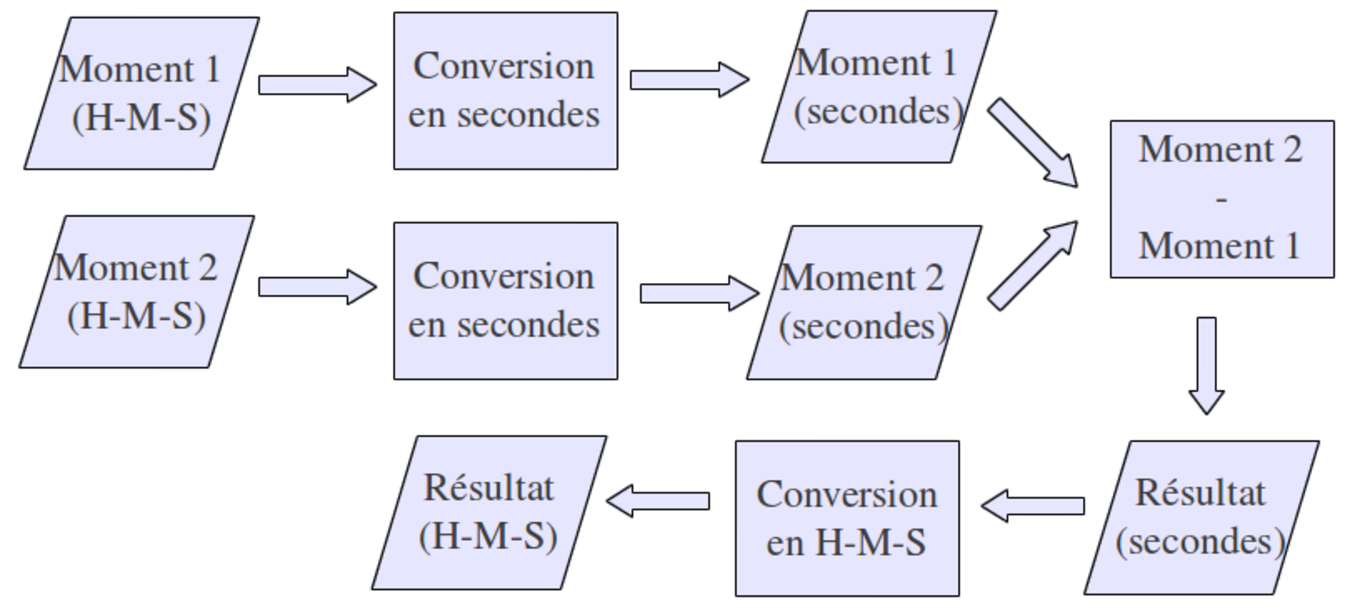
\includegraphics[width=0.8\textwidth]{image/module-conversion}
		\end{center}
	
	\subsection*{Conversion en secondes}
	
		Une des sous-tâches est donc la conversion en secondes
		d’un moment exprimé en heures-minutes-secondes
		(h-m-s). Il nous faut adapter la solution trouvée pour
		l’exercice du chapitre sur les algorithmes séquentiels
		car il n’est pas question ici que les données soient
		lues ni que le résultat soit écrit~; l’interaction ne
		se fait pas avec l’utilisateur mais avec le module
		principal qui va l’utiliser%
		\footnote{%
			On pourrait, dans notre cas précis, 
			imaginer que le module de conversion demande les données 
			à l’utilisateur mais un tel module serait
			moins souvent réutilisable.
		}.
	
		La première question à se poser est donc celle des paramètres~:
	
		\begin{liste}
		\item 
			Quelles sont les données dont a besoin l’algorithme
			pour travailler~?
		\item 
			Quels résultats fournit-il~?
		\end{liste}
	
		Dans notre cas, la réponse est simple~:
	
		\begin{liste}
		\item
			Les données sont le moment à convertir en secondes. 
			Ce moment est représenté par trois entiers~:~
			les heures, les minutes et les secondes ;
		\item
			Le résultat est le moment converti en secondes. 
			Il est représenté par un entier.
		\end{liste}
	
		Lorsque le résultat est représenté par une seule donnée, 
		on a le choix entre un paramètre en sortie~:
	
		\begin{Pseudocode}
			\LComment Reçoit trois entiers~:~des heures, des minutes et des secondes 
			\LComment et sort le nombre de secondes correspondant.
			\ModuleSign{hmsVersSec}{h\In, m\In, s\In, secondes\Out~:~entiers}{}
		\end{Pseudocode}
		
		ou une valeur de retour~:
	
		\begin{Pseudocode}
			\LComment Reçoit trois entiers~: des heures, des minutes et des secondes 
			\LComment et retourne le nombre de secondes correspondant.
			\ModuleSign{hmsVersSec}{h\In, m\In, s\In~: entiers}{entier}
		\end{Pseudocode}
	
		Dans de pareils cas, 
		on privilégie souvent la valeur de retour car cela
		facilite l’écriture lors de l’appel.
	
		L’algorithme s’écrit alors~:
	
		\begin{Pseudocode}
			\LComment Reçoit trois entiers~:~des heures, des minutes et des secondes 
			\LComment et retourne le nombre de secondes correspondant.
			\Module{hmsVersSec}{h\In, m\In, s\In~: entiers}{entier}
				\Decl secondes~:~entier \RComment {À déclarer puisque ce n’est pas un paramètre}
				\Let secondes \Gets  h * 3600 + m * 60 + s
				\Return secondes
			\EndModule
		\end{Pseudocode}
	
		ou de manière équivalente mais plus concise~:
	
		\begin{Pseudocode}
			\LComment Reçoit trois entiers~:~des heures, des minutes et des secondes 
			\LComment et retourne le nombre de secondes correspondant.
			\Module{hmsVersSec}{h\In, m\In, s\In~:~entiers}{entier}
				\Return h * 3600 + m * 60 + s
			\EndModule
		\end{Pseudocode}
	
	\subsection{Conversion en heures-minutes-secondes}
	
		À la fin de notre algorithme, il nous faudra reconvertir un résultat
		exprimé en secondes sous la forme heures-minutes-secondes. 
		À nouveau, on a déjà résolu ce problème 
		dans le chapitre sur les algorithmes séquentiels. 
		Mais il faut l’adapter à l’usage de paramètres.
	
		\begin{liste}
		\item
			Quelles sont les données~? Une seule, le moment exprimé en secondes
		\item
			Quels sont les résultats calculés par le module~? 
			Ce même moment exprimé en heures-minutes-secondes. 
			Trois entiers sont requis ce qui fait que le choix 
			entre un paramètre en sortie et une valeur de retour ne se
			pose pas ici~; 
			impossible d’utiliser une valeur de retour 
			(qui doit être unique)~; 
			on doit utiliser des paramètres en sortie.
		\end{liste}
	
		Ce qui donne~:
	
		\begin{Pseudocode}
			\LComment Reçoit un nombre de secondes et sort les heures, 
				les minutes et les secondes correspondant.
			\Module{secVersHMS}{secondes\In, h\Out, m\Out, s\Out~: entiers}{}
				\Let h \Gets secondes DIV 3600
				\Let m \Gets (secondes MOD 3600) DIV 60
				\Let s \Gets secondes MOD 60
			\EndModule
		\end{Pseudocode}
	
	\subsection{La solution}
	
		À présent, on a tout pour écrire la solution à notre problème
	
		\begin{Pseudocode}
			\LComment Lit deux moments (h-m-s) et affiche le moment de la différence entre les deux.
			\Module{différenceEntreHeures}{}{} \RComment Pas de paramètre~!
				\Decl h1, m1, s1, h2, m2, s2~:~entiers \RComment Les 2 moments à soustraire
				\Decl secondes1, secondes2~:~entiers \RComment Ces 2 moments en secondes
				\Decl diffSecondes~:~entier \RComment La différence en secondes
				\Decl diffH, diffM, diffS~:~entiers \RComment La différence en H-M-S
				\Read h1, m1, s1, h2, m2, s2
				\Let secondes1 \Gets hmsVersSec( h1, m1, s1 )
				\Let secondes2 \Gets hmsVersSec( h2, m2, s2 )
				\Let diffSecondes \Gets secondes2 – secondes1
				\Stmt secVersHMS( diffSecondes, diffH, diffM, diffS )
				\Write diffH, diffM, diffS
			\EndModule
		\end{Pseudocode}
	
		
		\begin{Emphase}[reflexion]{Réflexion}
			Dans la solution ci-dessus, 
			quelle est ou quelles sont la/les variable(s) locale(s) 
			dont on pourrait se passer moyennant une réécriture de
			l’algorithme~?
		\end{Emphase}
	
\section{Blocs}
% =============
	
	Un bloc est l’écriture d’une portion de module à l’extérieur de celui-ci. 
	C’est un simple \textit{déplacement} de lignes de code 
	vers un autre endroit du texte de l’algorithme. 
	La raison de découper un module en blocs peut être 
	le souci de clarifier un algorithme en le découpant en étapes
    bien distinctes, ou tout simplement un manque de place. 
    Les variables d’un bloc ne sont donc pas des variables locales 
    du bloc dans lequel elles apparaissent, 
    mais bien des variables locales du module auquel appartient ce bloc. 
    L’appel de l’exécution des instructions se trouvant
	dans un bloc est similaire à celui d’un module avec paramètres, 
	on écrit simplement le nom du bloc comme s’il s’agissait d’une
	instruction.

	Pour exemple, le module \pseudocode{additionnerFractions} 
	(première version dans le chapitre sur les algorithmes séquentiels) 
	pourrait se découper ainsi~:

	\begin{Pseudocode}
	\LComment Lit les contenus de 2 fractions et affiche leur somme
		\Module{additionnerFractions}{}{}
			\Stmt déclaration
			\Stmt lectureDonnées
			\Stmt calculs
			\Stmt écritureRésultat
		\EndModule
	\end{Pseudocode}

	\begin{Pseudocode}
	\Block{déclaration}
		\Decl num1, den1, num2, den2, numRes, denRes~:~entiers
	\EndBlock
	\end{Pseudocode}

	\begin{Pseudocode}
	\Block{lectureDonnées}
		\Read num1, den1, num2, den2
	\EndBlock
	\end{Pseudocode}

	\begin{Pseudocode}
	\Block{calculs}
		\Let numRes \Gets num1 * den2 + num2 * den1
		\Let denRes \Gets den1 * den2
	\EndBlock
	\end{Pseudocode}

	\begin{Pseudocode}
	\Block{écritureRésultat}
		\Write numRes, "/", denRes \RComment la fraction n’est pas simplifiée
	\EndBlock
	\end{Pseudocode}

	Le bloc contenant la déclaration des variables
	est aussi appelé \textbf{dictionnaire des variables} du module.

\section{Qu’est-ce qu’un algorithme de qualité~?}
% ===============================================

	Nous voulons tous produire du code de qualité 
	mais qu’est-ce que cette notion recouvre vraiment~?
	Qu’est-ce qui permet de juger de la qualité d’un code~? 
	De nombreux critères existent. 
	Citons ici, parmi les plus pertinents, 
	ceux qui sont le plus liés à ce cours%
	\footnote{%
		Pour approfondir cette notion,
		l’étudiant pourra lire par exemple~:~
		Bertrand Meyer,
		«~\textit{Conception et programmation par objets~:~
		pour du logiciel de qualité}~», 
		aux éditions «\textit{~interéditions~}»
	}.

	\subsection{La validité}
	
		C’est l’évidence, le code doit réaliser les tâches 
		pour lesquelles il a été écrit, 
		même dans tous les cas particuliers imaginés. 
		C’est là le critère principal et les autres ne sont là 
		que pour aider à atteindre celui-ci plus facilement. 
		Ne nous leurrons pas, 
		ce critère est loin d’être facile à rencontrer. 
		Il suffit pour s’en convaincre de se rappeler toutes les fois 
		où des logiciels pourtant courants que nous utilisons 
		se sont déjà arrêtés sur des erreurs.
	
	\subsection{L’extensibilité (ou évolutivité)}
	
		Un code valide résout un problème particulier. 
		Mais dans les situations réelles, 
		le problème change régulièrement. 
		Nous voudrons adapter le logiciel à de nouveaux besoins, 
		à une modification de la législation,
		parce qu’un besoin était mal compris\dots{}
		Ces modifications peuvent parfois être prévues mais pas toujours.
	
		Le code doit être écrit de telle sorte qu’un changement
		mineur dans le problème n’implique
		qu’un changement mineur dans le code. 
		Ce changement doit être évident, facile à opérer et rapide. 
		Il ne doit pas mettre à mal la validité du code.
	
	\subsection{La réutilisabilité}
	
		On désigne par ce terme la capacité de réutiliser 
		un bout de code d’un projet dans un autre projet de 
		façon aisée et sûre. L’avantage est de pouvoir employer 
		à nouveau un code qui a déjà fait ses preuves dans le 
		but de gagner du temps que l’on pourra investir dans les 
		aspects algorithmiques propres au nouveau projet. 
		Le découpage en modules joue ici un rôle essentiel.
	
	\subsection{La lisibilité}
	
		La lisibilité d’un code recouvre une notion globale et locale. 
		Au niveau global, on doit facilement comprendre 
		la structure générale du code 
		afin de pouvoir aisément comprendre 
		où se trouve la portion de code qui nous intéresse. 
		Au niveau local, on doit pouvoir comprendre
		aisément chaque bout de code.
	
		Au niveau du procédural (on nomme ainsi la programmation qui se
		structure à l’aide de modules), cela revient à dire
		qu’on doit rapidement voir quelles sont les fonctions et
		leur rôle (niveau global) et que chaque fonction sera aisément
		compréhensible (niveau local).
		
		Est-ce que la lisibilité d’un code passe par
		l’abondance de commentaire~? 
		Non, pas forcément. 
		Le commentaire sert à expliquer 
		ce qui n’est pas immédiatement clair dans le code. 
		La première source de lisibilité provient donc du code lui-même. 
		C’est pourquoi on est attentif à la bonne découpe en modules, 
		au choix judicieux des noms de modules et de variables\dots{}
		Le respect de ces bonnes pratiques 
		diminue le besoin de commentaires.
		
	\subsection{L’efficience}
	
		Ce critère s’intéresse à la bonne utilisation des
		ressources informatiques. Est-ce que le programme va tourner
		suffisamment vite, utiliser peu de mémoire~? Faut-il chercher
		systématiquement à optimiser son code~? Non~! On a souvent tendance à
		surévaluer ce critère ce qui est dommageable pour trois raisons.
	
		\begin{liste}
		\item
			Souvent, l’approche directe est suffisante. 
			Par exemple, la plupart des applications sont interactives.
			C’est alors l’utilisateur qui est le plus lent, 
			pas la machine qui a tout le temps d’effectuer sa tâche
			pendant que l’utilisateur réfléchit à ce qu’il doit taper.
		\item 
			En général, un programme passe 80\% de son temps dans 20\% de son code.
			Chercher à optimiser chaque ligne de code est une perte de temps.
		\item 
			Accroitre la rapidité d’un code est presque toujours 
			en contradiction avec sa lisibilité. 
			On risque d’utiliser un algorithme moins connu 
			ou des raccourcis difficiles à suivre.
		\end{liste}
	
		C’est pourquoi on recommande en général, face à un problème, 
		d’utiliser la solution la plus courante, la plus claire. 
		Une fois le programme terminé, 
		et seulement si le besoin s’en fait sentir, 
		on identifiera les portions de code où le programme s’attarde 
		le plus et on cherchera à les optimiser.
	
\clearpage
\section{Exercices}
% =================

\begin{Exercice}{Compréhension}
	Indiquer quels nombres sont successivement affichés lors de l’exécution
	des modules ex1, ex2, ex3 et ex4.

	\begin{Pseudocode}
	\Module{ex1}{}{}
		\Decl x, y~:~entiers
		\Stmt addition(3, 4, x)
		\Write x
		\Let x \Gets 3
		\Let y \Gets 5
		\Stmt addition(x, y, y)
		\Write y
	\EndModule

	\Empty

	\Module{addition}{a\In, b\In, c\Out~:~entiers}{}
		\Decl somme~:~entier
		\Let somme \Gets a + b
		\Let c \Gets somme
	\EndModule
	\end{Pseudocode}

	\begin{Pseudocode}
	\Module{ex2}{}{}
		\Decl a, b~:~entiers
		\Stmt addition(3, 4, a) \Comment voir ci-dessus
		\Write a
		\Let a \Gets 3
		\Let b \Gets 5
		\Stmt addition(b, a, b)
		\Write b
	\EndModule
	\end{Pseudocode}

	\begin{Pseudocode}
	\Module{ex3}{}{}
		\Decl a, b, c~:~entiers
		\Stmt calcul(3, 4, c)
		\Write c
		\Let a \Gets 3
		\Let b \Gets 4
		\Let c \Gets 5
		\Stmt calcul(b, c, a)
		\Write a, b, c
	\EndModule
	\Empty
	\Module{calcul}{a\In, b\In, c\Out~:~entiers}{}
		\Let a \Gets 2 * a
		\Let b \Gets 3 * b
		\Let c \Gets a + b
	\EndModule
	\end{Pseudocode}

	\begin{Pseudocode}
	\Module{ex4}{}{}
		\Decl a, b, c~:~entiers
		\Let a \Gets 3
		\Let b \Gets 4
		\Let c \Gets f(b)
		\Write c
		\Stmt calcul2(a, b, c)
		\Write a, b, c
	\EndModule
	\Empty
	\Module{calcul2}{a\In, b\In, c\Out~:~entiers}{}
		\Let a \Gets f(a)
		\Let c \Gets 3 * b
		\Let c \Gets a + c
	\EndModule
	\Empty
	\Module{f}{a\In~:~entier}{entier}
		\Decl b~: entier
		\Let b \Gets 2 * a + 1
		\Return b
	\EndModule
	\end{Pseudocode}

\end{Exercice}

\begin{Exercice}{Appels de module}
	Parmi les instructions suivantes (où les variables
	\pseudocode{a}, \pseudocode{b} et \pseudocode{c}
	sont des entiers), lesquelles font correctement appel au module
	d’en-tête suivant~?

	\begin{Pseudocode}
		\ModuleSign{PGCD}{a\In,b\In~:~entiers}{entier}
	\end{Pseudocode}

	\begin{Pseudocode}
	\Stmt [1] a \Gets PGCD(24, 32)
	\Stmt [2] a \Gets PGCD(a, 24)
	\Stmt [3] b \Gets 3 * PGCD(a + b, 2*c) + 120
	\Stmt [4] PGCD(20, 30)
	\Stmt [5] a \Gets PGCD(a, b, c)
	\Stmt [6] a \Gets PGCD(a, b) + PGCD(a, c)
	\Stmt [7] a \Gets PGCD(a, PGCD(a, b))
	\Stmt [8] \K{lire} PGCD(a, b)
	\Stmt [9] \K{afficher} PGCD(a, b)
	\Stmt [10] PGCD(a, b) \Gets c
	\end{Pseudocode}
\end{Exercice}

\begin{Exercice}{Comparaison d’algorithmes}
	Soit un module testant si un nombre entier est pair.
	Comparez les différentes solutions proposées.

	\begin{Pseudocode}
		\LComment Affiche un entier et retourne vrai s’il est pair et faux sinon.
		\Module{estPair}{nb\In~:~entier}{booléen}
		\Decl pair~:~booléen
		\Let pair \Gets faux
		\If{nb MOD 2 = 0}
			\Let pair \Gets vrai
		\EndIf
		\Return pair
		\EndModule
	\end{Pseudocode}

	\begin{Pseudocode}
		\LComment Affiche un entier et retourne vrai s’il est pair et faux sinon.
		\Module{estPair}{nb\In~:~entier}{booléen}
		\Decl pair~:~booléen
		\If{nb MOD 2 = 0}
			\Let pair \Gets vrai
		\Else
			\Let pair \Gets faux
		\EndIf
		\Return pair
		\EndModule
	\end{Pseudocode}

	\begin{Pseudocode}
		\LComment Affiche un entier et retourne vrai s’il est pair et faux sinon.
		\Module{estPair}{nb\In~:~entier}{booléen}
			\Decl pair~:~booléen
			\Let pair \Gets nb MOD 2 = 0
			\Return pair
		\EndModule
	\end{Pseudocode}

	\begin{Pseudocode}
		\LComment Affiche un entier et retourne vrai s’il est pair et faux sinon.
		\Module{estPair}{nb\In~:~entier}{booléen}
		\Return nb MOD 2 = 0
		\EndModule
	\end{Pseudocode}

	\begin{Pseudocode}
		\LComment Affiche un entier et retourne vrai s’il est pair et faux sinon.
		\Module{estPair}{nb\In~:~entier}{booléen}
		\If{nb MOD 2 = 0}
			\Return vrai
		\Else
			\Return faux
		\EndIf
		\EndModule
	\end{Pseudocode}

	\begin{Pseudocode}
		\LComment Affiche un entier et retourne vrai s’il est pair et faux sinon.
		\Module{estPair}{nb\In~:~entier}{booléen}
		\If{nb MOD 2 = 0}
			\Return vrai
		\EndIf
		\Return faux
		\EndModule
	\end{Pseudocode}	
\end{Exercice}

\begin{Exercice}{Échange de variables}
	\marginicon{java}
	Écrire un module \textit{swap} qui échange le contenu de deux variables
	entières passées en paramètres.
\end{Exercice}

\begin{Exercice}{Valeur absolue}
	Écrire un module qui retourne la valeur absolue d’un
	réel reçu en paramètre.
	Quel est l’avantage pour un module de retourner la réponse 
	plutôt que de l’afficher~?
\end{Exercice}

\begin{Exercice}{Maximum de 4 nombres}
	\marginicon{java}
	Écrire un module qui retourne le maximum de 4
	nombres donnés en paramètre en utilisant les modules
	max2 et/ou max3 déjà développés dans ce chapitre.
\end{Exercice}

\begin{Exercice}{Validité d’une date}
	\marginicon{java}
	Reprendre l’algorithme de validation d’une date 
	développé au chapitre précédent et le rendre modulaire.
\end{Exercice}


% ==================================
\chapter{Les variables structurées}
% ==================================

% ==========================
\section{Le type structuré}
% ==========================

	Dans les chapitres précédents, nous avons utilisé des variables de types
	dits «~simples~» (entier, réel, booléen, caractère, chaine) ne pouvant
	contenir qu’une seule valeur à la fois. Cependant, certains types
	d’information consistent en un regroupement de plusieurs données
	élémentaires. Quelques exemples~:

	\begin{liste}
	\item
		Une \textbf{date} est composée de trois éléments (le jour, le mois,
		l’année). Le mois peut s'exprimer par un entier (15/10/2014) 
		ou par une chaine (15~octobre~2014).
	\item
		Un \textbf{moment} de la journée est un triple d’entiers 
		(heures, minutes, secondes).
	\item
		La localisation d’un \textbf{point} dans un plan 
		nécessite la connaissance de deux coordonnées cartésiennes 
		(l’abscisse \textit{x} et l’ordonnée \textit{y}) 
		ou polaires 
		(le rayon \textit{r} et l’angle \textit{$\theta$}).
	\item
		Une \textbf{adresse} est composée de plusieurs données~:~
		un nom de rue, 
		un numéro de maison, 
		parfois un numéro de boite postale, 
		un code postal, 
		le nom de la localité, 
		un nom ou code de pays pour une adresse à l’étranger\dots
	\end{liste}

	Pour stocker et manipuler de tels ensembles de données, nous utiliserons
	des \textbf{types structurés} ou \textbf{structures}\footnote{Nous
	verrons dans un chapitre ultérieur que l’approche
	«~orientée objet~» offre également une solution élégante pour manipuler
	des données complexes.}. Une \textbf{structure} est donc un ensemble
	fini d’éléments pouvant être de types distincts. Chaque élément de cet
	ensemble, appelé \textbf{champ} de la structure, possède un nom unique.
	
	Notez qu’un champ d’une structure peut lui-même être une structure. Par
	exemple, une \textbf{carte d’identité} inclut parmi ses informations
	une \textbf{date} de naissance, l’\textbf{adresse} de son
	propriétaire (cachée dans la puce électronique~!)\dots

% ===================================
\section{Définition d’une structure}
% ===================================

	\marginicon{definition}
	La définition d’un type structuré adoptera le modèle suivant~:

	\begin{Pseudocode}
	\Struct{NomDeLaStructure}
		\Decl nomChamp1 : type1
		\Decl nomChamp2 : type2
		\Decl \dots
		\Decl nomChampN : typeN
	\EndStruct
	\end{Pseudocode}

	\pseudocode{nomChamp1}, \dots, \pseudocode{nomChampN} 
	sont les noms des différents champs de la structure, 
	et \pseudocode{type1}, \dots, \pseudocode{typeN} 
	les types de ces champs. 
	Ces types sont soit les types «~simples~» étudiés
	précédemment (entier, réel, booléen, caractère, chaine) soit d’autres
	types structurés dont la structure aura été préalablement définie.

	Pour exemple, nous définissons ci-dessous trois
	types structurés que nous utiliserons souvent par la suite~:

	\begin{minipage}{4.5cm}
	\begin{Pseudocode}
	\Struct{Date}
		\Decl jour : entier
		\Decl mois : entier
		\Decl année : entier
	\EndStruct
	\end{Pseudocode}
	\end{minipage}
\ 
	\begin{minipage}{4.5cm}
	\begin{Pseudocode}
	\Struct{Moment}
		\Decl heure : entier
		\Decl minute : entier
		\Decl seconde : entier
	\EndStruct
	\end{Pseudocode}
	\end{minipage}
\ 
	\begin{minipage}{4.5cm}
	\begin{Pseudocode}
	\Struct{Point}
		\Decl x : réel
		\Decl y : réel
	\EndStruct{}
	\Empty
	\end{Pseudocode}
	\end{minipage}

% =====================================================
\section{Déclaration d’une variable de type structuré}
% =====================================================

	Une fois un type structuré défini, 
	la déclaration de variables de ce type 
	est identique à celle des variables simples. 
	Par exemple~:

	\begin{Pseudocode}
	\Decl anniversaire, jourJ : Date
	\Decl départ, arrivée, unMoment : Moment
	\Decl a, b, centreGravité : Point
	\end{Pseudocode}

% ====================================================
\section{Utilisation des variables de type structuré}
% ====================================================

	En général, 
	pour manipuler une variable structurée ou en modifier le contenu, 
	il faut agir au niveau de ses champs en utilisant 
	les opérations permises selon leur type. 
	Pour accéder à l’un des champs d’une variable structurée, 
	il faut mentionner le nom de ce champ 
	ainsi que celui de la variable dont il fait partie.
	Nous utiliserons la notation «~pointée~»~:

	\begin{Pseudocode}
	\Stmt nomVariable.nomChamp
	\end{Pseudocode}

	Exemple d’instructions utilisant les variables
	déclarées au paragraphe précédent~:

	\begin{Pseudocode}
	\Let anniversaire.jour \Gets 15
	\Let anniversaire.mois \Gets 10
	\Let anniversaire.année \Gets 2014
	\Let arrivée.heure \Gets départ.heure + 2
	\Let centreGravité.x \Gets (a.x + b.x) / 2
	\end{Pseudocode}

	On peut cependant, dans certains cas, 
	utiliser une variable structurée de manière globale 
	(c’est-à-dire d’une façon qui agit simultanément sur chacun de ses champs). 
	Le cas le plus courant est l’affectation interne 
	entre deux variables structurées de même type, 
	par exemple~:

	\begin{Pseudocode}
	\Let arrivée \Gets départ
	\end{Pseudocode}

	qui résume les trois instructions suivantes~:

	\begin{Pseudocode}
	\Let arrivée.heure \Gets départ.heure
	\Let arrivée.minute \Gets départ.minute
	\Let arrivée.seconde \Gets départ.seconde
	\end{Pseudocode}

	Une variable structurée peut aussi être le paramètre d’un module, 
	et un module peut également renvoyer une «~valeur~» de type structuré. 
	Par exemple, l’entête d’un module renvoyant le nombre de secondes 
	écoulées entre une heure de départ et d’arrivée serait~:

	\begin{Pseudocode}
	\ModuleSign{nbSecondesEcoulées}{ départ\In, arrivée\In : Moment}{entier}
	\end{Pseudocode}

	On pourra aussi lire ou afficher une variable structurée%
	\footnote{%
		Bien que, dans certains langages, 
		ces opérations devront être décomposées en une lecture ou
		écriture de chaque champ de la structure.
	}.

	\begin{Pseudocode}
	\Read unMoment
	\Write unMoment
	\end{Pseudocode}

	Par contre, il n’est pas autorisé d’utiliser
	les opérateurs de comparaison ({\textless}, {\textgreater}) 
	pour comparer des variables structurées (même de même type), 
	car une relation d’ordre n’accompagne pas toujours les structures utilisées. 
	En effet, s’il est naturel de vouloir comparer des dates ou des moments,
	comment définir une relation d’ordre avec les points du plan ou avec
	des cartes d’identités~?

	Si le besoin de comparer des variables structurées se fait sentir, 
	il faudra dans ce cas écrire 
	des modules de comparaison adaptés aux structures utilisées.

	Par facilité d’écriture, 
	on peut assigner tous les champs en une fois via des «~\{\}~». 
	Exemple~:

	\begin{Pseudocode}
	\Let anniversaire \Gets \{1, 9, 1989\}
	\end{Pseudocode}

% =============================
\section{Exemple d’algorithme}
% =============================

	Le module ci-dessous reçoit en paramètre deux dates ; 
	la valeur renvoyée est 
	–1 si la première date est antérieure à la deuxième, 
	0 si les deux dates sont identiques 
	ou 1 si la première date est postérieure à la deuxième.

	\begin{Pseudocode}
	\LComment Reçoit 2 dates en paramètres et retourne la valeur
	\LComment {–1 si la première date est antérieure à la deuxième}
	\LComment 0 si les deux	dates sont identiques
	\LComment 1 si la première date est postérieure à la deuxième.
	\Module{comparerDates}{date1\In, date2\In : Date}{entier}
		\Decl résultat : entier
		\Let  résultat \Gets -1
		\RComment valeur choisie par défaut
		\If{date1.année ${\geq}$ date2.année}
			\If{date1.année $>$ date2.année}
				\Let  résultat \Gets 1
			\Else \RComment les années sont identiques
				\If{date1.mois ${\geq}$ date2.mois}
					\If{date1.mois $>$ date2.mois}
						\Let  résultat \Gets 1
					\Else \RComment les années et les mois sont identiques
						\If{date1.jour ${\geq}$ date2.jour}
							\If{date1.jour $>$ date2.jour}
								\Let  résultat \Gets 1
							\Else \RComment les années, les mois et les jours sont identiques
								\Let  résultat \Gets 0
							\EndIf
						\EndIf
					\EndIf
				\EndIf
			\EndIf
		\EndIf
		\Return résultat
	\EndModule
	\end{Pseudocode}

% =====================================
\section{Exercices sur les structures}
% =====================================

\begin{Exercice}{Conversion moment-secondes}
	Écrire un module qui reçoit en paramètre un
	moment d’une journée et qui retourne le nombre de secondes écoulées
	depuis minuit jusqu’à ce moment.
\end{Exercice}

\begin{Exercice}{Conversion secondes-moment}
	Écrire un module qui reçoit en paramètre un
	nombre de secondes écoulées dans une journée à partir de minuit et qui
	retourne le moment correspondant de la journée.
\end{Exercice}

\begin{Exercice}{Temps écoulé entre 2 moments}
	Écrire un module qui reçoit en paramètres deux
	moments d’une journée et qui retourne le nombre de secondes séparant
	ces deux moments.
\end{Exercice}

\begin{Exercice}{Milieu de 2 points}
	Écrire un module recevant les coordonnées de
	deux points distincts du plan et qui retourne les coordonnées du point
	situé au milieu des deux.
\end{Exercice}

\begin{Exercice}{Distance entre 2 points}
	Écrire un module recevant les coordonnées de
	deux points distincts du plan et qui retourne
	la distance entre ces deux points.
\end{Exercice}

\begin{Exercice}{Un cercle}
	Définir un type \textbf{Cercle} pouvant décrire de façon
	commode un cercle quelconque dans un espace à deux dimensions. 	
	Écrire ensuite
	
	\begin{enumerate}[label=\alph*)]
	\item {
		un module calculant la surface du cercle reçu en paramètre ;}
	\item {
		un module recevant 2 points en paramètre et retournant le cercle dont le
		diamètre est le segment reliant ces 2 points ;}
	\item {
		un module qui détermine si un point donné est dans un cercle ;}
	\item {
		un module qui indique si 2 cercles ont une intersection.
	}
	\end{enumerate}
\end{Exercice}


\begin{Exercice}{Un rectangle}
	\marginicon{java}
	Définir un type \textbf{Rectangle} pouvant décrire de façon
	commode un rectangle dans un espace à deux dimensions et dont les côtés
	sont parallèles aux axes des coordonnées. 	
	Écrire ensuite

	\begin{enumerate}[label=\alph*)]
	\item {
		un module calculant le périmètre d’un rectangle reçu en paramètre ;}
	\item {
		un module calculant la surface d’un rectangle reçu en paramètre ;}
	\item {
		un module recevant en paramètre un rectangle R et les coordonnées
		d’un point P, et renvoyant 
		\textbf{vrai} si et seulement si le point P est à
		l’intérieur du rectangle R ;}
	\item {
		un module recevant en paramètre un rectangle R et les coordonnées
		d’un point P, et renvoyant 
		\textbf{vrai} si et seulement si le point P est sur le bord du
		rectangle R ;}
	\item {
		un module recevant en paramètre deux rectangles et renvoyant la valeur
		booléenne \textbf{vrai} si et seulement si ces deux rectangles ont une
		intersection.}
	\end{enumerate}
\end{Exercice}

\begin{Exercice}{Validation de date}
	Écrire un algorithme qui valide une date reçue en paramètre 
	sous forme d’une structure.
\end{Exercice}

	

% ====================
\chapter{Les boucles}
\label{chap:bcl}
% ====================

	\marginicon{objectif}
	Les ordinateurs révèlent tout leur potentiel dans leur capacité à
	répéter inlassablement les mêmes tâches.
	Nous voyons ici comment incorporer des boucles dans nos codes 
	et comment les utiliser à bon escient.

	\marginicon{attention}
	Attention~! 
	D’expérience, nous savons que ce chapitre est difficile à appréhender. 
	Beaucoup d’entre vous perdent pied ici. 
	Accrochez-vous et faites bien tous les exercices proposés~!

% =======================================
\section{La notion de travail répétitif}
% =======================================

	Si on veut faire effectuer un travail répétitif, 
	il faut indiquer deux choses~:
	
	\begin{enumerate}
	\item Le travail à répéter
	\item La manière de continuer la répétition ou de l’arrêter.
	\end{enumerate}

	Examinons quelques exemples pour fixer notre propos.

	\textbf{Exemple 1}~: 
	Pour traiter des dossiers, 
	on dira quelque chose comme 
	«~tant qu’il reste un dossier à traiter, le traiter~» 
	ou encore 
	«~traiter un dossier puis passer au suivant jusqu’à ce qu’il n’en reste plus à traiter~».

	\begin{liste}
	\item La tâche à répéter est : «~traiter un dossier~»
	\item On indique qu’on doit continuer s’il reste encore un dossier à traiter.
	\end{liste}

	\textbf{Remarque~:}~
	On aurait aussi pu le formuler ainsi~:~
	«~traiter un dossier et passer au suivant jusqu’à ce qu’il n’en reste plus~».

	\textbf{Exemple 2}~:~
	Pour calculer la cote finale de tous les étudiants,
	on aura quelque chose du genre 
	«~Pour tout étudiant, calculer sa cote~».

	\begin{liste}
	\item 
		La tâche à répéter est : «~calculer la cote d’un étudiant~»
	\item 
		On indique qu’on doit le faire pour tous les étudiants.
		On doit donc commencer par le premier, passer à chaque fois au suivant
		et s’arrêter quand on a fini le dernier.
	\end{liste}

	\textbf{Exemple 3}~:~
	Pour afficher tous les nombres de 1 à 100, on aura
	«~Pour tous les nombres de 1 à 100, afficher ce nombre~».

	\begin{liste}
	\item
		La tâche à répéter est : «~afficher un nombre~»
	\item 
		On indique qu’on doit le faire pour tous les nombres de 1 à 100. 
		On doit donc commencer avec 1, 
		passer à chaque fois au nombre suivant 
		et s’arrêter après avoir affiché le nombre 100.
	\end{liste}

	\textbf{Attention}~! 
	Comprenez bien que c’est toujours la même tâche qui est exécutée 
	mais pas avec le même effet à chaque fois. 
	Ainsi, on traite un dossier mais à chaque fois un différent ; 
	on affiche un nombre mais à chaque fois un différent. 
	Nous verrons comment y arriver en logique.

% ==============================
\section{Structures itératives}
% ==============================

	Chacune des structures suivantes traduit une volonté de faire exécuter
	de façon répétée une séquence d’instructions. 

	\subsection{«~tant que~»}

		Le «~tant que~» est une structure qui demande à
		l’exécutant de répéter une tâche (une ou plusieurs
		instructions) tant qu’une condition donnée est vraie.

		\begin{Pseudocode}
		\While{condition}
			\Stmt séquence d’instructions à exécuter
		\EndWhile
		\end{Pseudocode}

		Comme pour la structure \pseudocode{si}, 
		la \pseudocode{condition} est une expression à valeur booléenne. 
		Dans ce type de structure, 
		il faut qu’il y ait dans la séquence d’instructions comprise entre
		\pseudocode{tant que} et \pseudocode{fin tant que} au moins une
		instruction qui modifie une des composantes de la condition de telle
		manière qu’elle puisse devenir \textbf{fausse} à un moment donné. Dans
		le cas contraire, la condition reste indéfiniment vraie et la boucle va
		tourner sans fin, c’est ce qu’on appelle une \textbf{boucle infinie}. 
		La figure \vref{fig:boucle-tq} est un ordinogramme 
		décrivant le déroulement de cette structure. 
		On remarquera que si la condition est fausse dès le début, 
		la tâche n’est jamais exécutée.

		\begin{figure}[h]
		\centering
		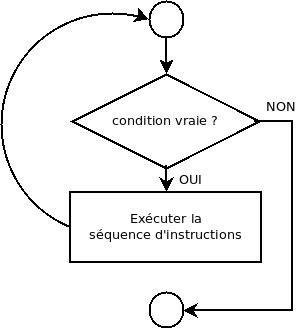
\includegraphics[width=0.5\textwidth]{image/boucle-tq}
		\caption{Ordinogramme de la boucle "tant-que"}
		\label{fig:boucle-tq}
		\end{figure}
		
	\subsection{«~faire~–~jusqu’à ce que~»}

		Cette structure est très proche du «~tant que~» 
		à deux différences près~:
	
		\begin{enumerate}
		\item
			Le test est fait à la fin et pas au début. 
			La tâche est donc toujours exécutée au moins une fois.
		\item 
			On donne la condition pour arrêter et pas pour continuer ; 
			il s’agit d’une différence mineure.
		\end{enumerate}

		\begin{Pseudocode}
		\Repeat
			\Stmt séquence d’instructions à exécuter
		\Until{condition}
		\end{Pseudocode}

		Comme ci-dessus, il faut que la séquence d’instructions comprise entre
		\pseudocode{faire} et \pseudocode{jusqu’à ce que} 
		contienne au moins une instruction qui modifie la condition de
		telle manière qu’elle puisse devenir \textbf{vraie} à un moment donné
		pour arrêter l’itération. 
		La figure \vref{fig:boucle-faire} décrit le déroulement de cette boucle. 

		\begin{figure}[h]
		\centering
		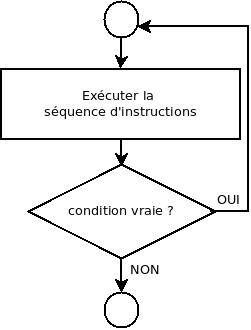
\includegraphics[width=0.4\textwidth]{image/boucle-faire}
		\caption{Ordinogramme de la boucle "faire – jusqu’à ce que"}
		\label{fig:boucle-faire}
		\end{figure}

	\subsection{«~pour~»}

		Ici, on va plutôt indiquer \textbf{combien de fois} la tâche doit être
		répétée. Cela se fait au travers d’une
		\textbf{variable de contrôle} dont la valeur va évoluer à partir
		d’une valeur de départ jusqu’à une
		valeur finale.
		
		\begin{Pseudocode}
		\For{variable \K{de} début \K{à} fin [\K{par} pas]}
			\Stmt séquence d’instructions à exécuter
		\EndFor
		\end{Pseudocode}

		Dans ce type de structure, 
		\pseudocode{début}, \pseudocode{fin} et \pseudocode{pas}
		peuvent être des constantes, des variables ou des expressions 
		(le plus souvent à valeurs entières mais on admettra parfois des réels). 
		Le \pseudocode{pas} est facultatif, et généralement omis 
		(dans ce cas, sa valeur par défaut est 1). 
		Ce pas est parfois négatif, dans le cas d’un compte à rebours, 
		par exemple \pseudocode{pour n de 10 à 1 par -1}.

		Quand le \pseudocode{pas} est positif, la boucle s’arrête
		lorsque la variable dépasse la valeur de \pseudocode{fin}. 
		Par contre, avec un \pseudocode{pas} négatif, 
		la boucle s’arrête lorsque la variable prend une valeur 
		plus petite que la valeur de \pseudocode{fin}
		(cf. le test dans l’organigramme de la figure \vref{fig:boucle-pour}).

		\begin{figure}[h]
		\centering
		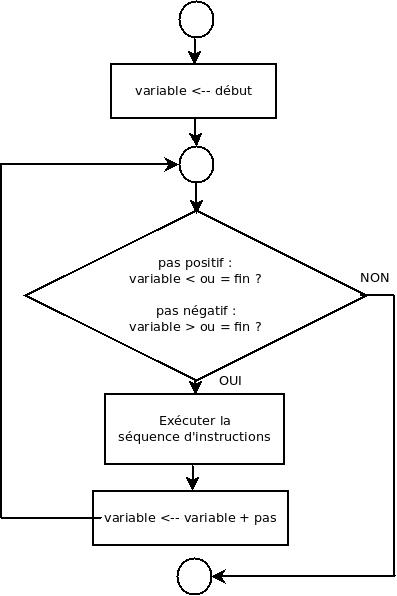
\includegraphics[width=0.5\textwidth]{image/boucle-pour}
		\caption{Ordinogramme de la boucle "pour"}
		\label{fig:boucle-pour}
		\end{figure}

		\marginicon{attention}
		Veiller à la cohérence de l’écriture de cette structure. On considérera
		qu’au cas (à éviter) où \pseudocode{début} est strictement supérieur à
		\pseudocode{fin} et le \pseudocode{pas} est positif, la séquence d’instructions
		n’est jamais exécutée (mais ce n’est pas le cas dans tous les langages
		de programmation~!). Idem si \pseudocode{début} est strictement inférieur à
		\pseudocode{fin} mais avec un \pseudocode{pas} négatif.

		\textbf{Exemples~}:

		\begin{Pseudocode}
		\Stmt \K{pour} i \K{de} 0 \K{à} 2 \K{faire} \RComment La boucle est exécutée 3 fois.
		\Stmt \K{pour} i \K{de} 2 \K{à} 0 \K{faire} \RComment La boucle n’est pas exécutée.
		\Stmt \K{pour} i \K{de} 1 \K{à} 10 \K{par} -1 \K{faire} \RComment La boucle n’est pas exécutée.
		\Stmt \K{pour} i \K{de} 1 \K{à} 1 \K{par} 5 \K{faire} \RComment La boucle est exécutée 1 fois.
		\end{Pseudocode}
		
		\marginicon{attention}
		Veiller aussi à ne pas modifier dans la séquence d’instructions une des
		variables de contrôle \pseudocode{début}, \pseudocode{fin} ou \pseudocode{pas}~! Il
		est aussi fortement déconseillé de modifier «~manuellement~» la
		\pseudocode{variable} de contrôle au sein de la boucle
		\pseudocode{pour}. Il ne faut pas l’initialiser en début de boucle,
		et ne pas s’occuper de sa modification, l’instruction 
		\pseudocode{variable \Gets variable + pas} 
		étant automatique et implicite à chaque étape de la
		boucle. Il est aussi déconseillé d’utiliser \pseudocode{variable} à la
		sortie de la structure \pseudocode{pour} sans lui affecter une
		nouvelle valeur (son contenu pouvant varier selon le langage de
		programmation).

	\subsection{Quel type de boucle choisir~?}

		En pratique, il est possible d’utiliser systématiquement la boucle 
		\pseudocode{tant que} qui peut s’adapter à toutes les situations. 
		Cependant, il est plus clair d’utiliser la boucle \pseudocode{pour} 
		dans les cas où le nombre d’itérations est fixé et connu à l’avance 
		(par là, on veut dire que le nombre d’itérations est déterminé au moment 
		où on arrive à la boucle). 
		La boucle \pseudocode{faire} convient quant à elle
		dans les cas où le contenu de la boucle doit être parcouru au moins une
		fois, alors que dans \pseudocode{tant que}, 
		le nombre de parcours peut être nul si la condition initiale est fausse. 
		La figure \vref{fig:boucle-choix} propose un petit schéma récapitulatif.

		\begin{figure}[h]
		\centering
		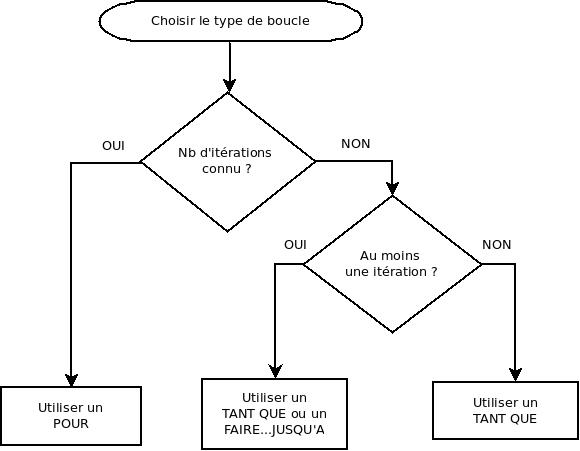
\includegraphics[width=0.8\textwidth]{image/boucle-choixtype}
		\caption{Quel type de boucle choisir~?}
		\label{fig:boucle-choix}
		\end{figure}

% =================
\section{Exemples}
% =================

	Nous présentons quelques exemples de difficulté
	croissante pour montrer comment bien utiliser les boucles.

	\subsection{Exemple 1 -- Compter de 1 à 10}

		Imaginons qu’on veuille afficher tous les nombres de 1 à 10. 
		On va évidemment rejeter cette première solution~:

		\begin{Pseudocode}
		\LComment Affiche les nombres de 1 à 10.
		\Module{compterJusque10}{}{} \RComment une mauvaise solution !
		\Write 1
		\Write 2
		\Write 3
		\Write 4
		\Write 5
		\Write 6
		\Write 7
		\Write 8
		\Write 9
		\Write 10
		\EndModule
		\end{Pseudocode}

		Non seulement c’est long à écrire 
		(imaginer l’algorithme pour afficher les nombres de 1 à 10000~!) 
		mais c’est très peu souple.
		Cela ne fonctionne que pour 10~:~il faut modifier l’algorithme pour
		un autre comptage. La boucle va nous permettre
		d’obtenir un algorithme qui s’adapte
		à la limite du décompte.

		Posons-nous les bonnes questions pour déterminer la boucle~:

		\begin{liste}
		\item 
			Quelle est la tâche à répéter~? Afficher un nombre.
		\item 
			Comment savoir si on continue~? On arrête quand «~10~» est affiché.
		\item 
			Comment afficher à chaque fois un nombre différent~? 
			Au travers d’une variable qui prendra toutes les valeurs de 1 à 10. 
			Il faut donc ajouter dans le corps de la
			boucle une incrémentation de la variable
		\end{liste}

		Ce qui donne~:

		\begin{Pseudocode}
		\LComment Affiche les nombres de 1 à 10.
		\Module{compterJusque10}{}{} \RComment version avec tant que
			\Decl nb : entier
			\Let nb \Gets 1 \RComment c’est le premier nombre à afficher
			\While{nb $\leq$ 10} \RComment tant que le nb à afficher est toujours bon
				\Write nb \RComment on affiche la valeur de la variable nb
				\Let nb \Gets nb + 1 \RComment on passe au nombre suivant
			\EndWhile
		\EndModule
		\end{Pseudocode}

		Mais ici, on pourrait aussi l’écrire avec un «~pour~» vu qu’on
		connait exactement le nombre d’exécutions de la boucle (10). 
		La variable de contrôle va évoluer de 1 à 10 ce qui tombe bien car
		c’est justement le nombre à afficher à chaque fois.

		\begin{Pseudocode}
		\LComment Affiche les nombres de 1 à 10.
		\Module{compterJusque10}{}{} \RComment version avec pour
			\Decl nb : entier
			\For{nb \K{de} 1 \K{à} 10} \RComment par défaut le pas est de 1
				\Write nb 
			\EndFor
		\EndModule
		\end{Pseudocode}

		On obtient une solution plus courte et plus lisible 
		car l’en-tête du «~pour~» indique clairement
		comment va évoluer la boucle
		(valeur de départ, pas et valeur finale)

	\subsection{Exemple 2 -- Compter de 1 à beaucoup}

		Dans l’exercice précédent, on a
		affirmé que la boucle pouvait s’adapter à la limite du
		décompte. Montrons-le~! Supposons qu’on veuille
		afficher les nombres de 1 à $n$ où $n$ est une valeur 
		donnée par l’utilisateur.

		Rien de plus simple, il suffit de lire cette
		valeur au début et de l’utiliser comme limite de boucle

		\begin{Pseudocode}
		\LComment Lit un nombre et affiche les nombres de 1 à ce nombre.
		\Module{afficherN}{}{} 
			\Decl nb, n : entier
			\Read n
			\For{nb \K{de} 1 \K{à} n} 
				\Write nb 
			\EndFor
		\EndModule
		\end{Pseudocode}

		\marginicon{reflexion}
		\textbf{Réflexion}~: Que se passe-t-il si l’utilisateur entre une valeur négative~?
		Comment améliorer le code pour que le programme
		le signale à l’utilisateur~?

	\subsection{Exemple 3 -- Afficher les nombres pairs}

		Cela se complique un peu. Cette fois-ci on
		affiche uniquement les nombres \textbf{pairs} jusqu’à la limite $n$.
		
		\textbf{Exemple}~:~les nombres pairs de $1$ à $10$ sont~: $2$, $4$, $6$, $8$, $10$.
		
		Notez que $n$ peut être impair. Si $n$ vaut $11$, 
		l’affichage est le même que pour $10$.

		Est-ce qu’on peut utiliser un «~pour~»~? 
		Oui. De 1 à $n$, il y a exactement «~$n$ DIV $2$~» nombres à afficher. 
		La difficulté vient du lien à faire entre la variable de
		contrôle et le nombre à afficher.

		\textbf{Solution 1}~:~on garde le lien entre la variable de contrôle 
		et le nombre à afficher. 
		Dans ce cas, on commence à $2$ et le pas doit être de $2$.

		\begin{Pseudocode}
		\LComment Lit un nombre et affiche les nombres pairs jusqu’à ce nombre.
		\Module{afficherPair}{}{} 
			\Decl nb, n : entier
			\Read n
			\RComment limite des nombres à afficher
			\For{nb \K{de} 2 \K{à} n \K{par} 2} 
				\Write nb 
			\EndFor
		\EndModule
		\end{Pseudocode}

		\textbf{Solution 2}~:~la variable de contrôle compte simplement 
		le nombre d’itérations.
		Alors il faut calculer le nombre à afficher en fonction de la variable
		de contrôle (ici le double de celle-ci convient)

		\begin{Pseudocode}
		\LComment Lit un nombre et affiche les nombres pairs jusqu’à ce nombre.
		\Module{afficherPair}{}{} 
			\Decl i, n : entier
			\Read n
			\RComment limite des nombres à afficher
			\For{i \K{de} 1 \K{à} n DIV 2} 
				\Write 2 * i 
			\EndFor
		\EndModule
		\end{Pseudocode}

		Par une vieille habitude des programmeurs%
		\footnote{%
			Née avec le langage FORTRAN 
			où la variable $i$ était par défaut une variable entière.
		},
		une variable de contrôle qui se contente de compter les passages dans
		la boucle est souvent nommée $i$. 
		On l’appelle aussi «~itérateur~».

	\subsection{Exemple 4 -- Afficher les premiers nombres pairs}

		Voici un problème proche du précédent~:~on affiche cette fois 
		les $n$ premiers nombres pairs.
		
		\textbf{Exemple}~:~les $10$ premiers nombres pairs sont~:~$2$, $4$, $6$, $8$, 
		$10$, $12$, $14$, $16$, $18$, $20$.
		
		Il est plus simple de partir de la solution 2 de l’exemple précédent
		en changeant simplement la valeur finale de la boucle.

		\begin{Pseudocode}
		\LComment Lit un nombre et affiche ce nombre de nombres pairs.
		\Module{afficherPair}{}{} 
			\Decl i, n : entier
			\Read n
			\RComment le nombre de nombres à afficher
			\For{i \K{de} 1 \K{à} n} 
				\Write 2 * i 
			\EndFor
		\EndModule
		\end{Pseudocode}

	\subsection{Exemple 5 -- Somme de nombres}

		Changeons de problème. On veut pouvoir calculer (et retourner)
		la somme d’une série de nombres donnés par
		l’utilisateur. Il faut d’abord se
		demander comment l’utilisateur va pouvoir indiquer
		combien de nombres il faut additionner ou quand est-ce que le dernier
		nombre à additionner a été entré. Voyons quelques possibilités.

		\medskip
		\textbf{Variante 1}~: 
		
		L’utilisateur indique le nombre de termes au départ.
		Ce problème est proche de ce qui a déjà été fait.
		
		\begin{Pseudocode}
		\LComment Lit des valeurs entières et retourne la somme des valeurs lues.
		\Module{sommeNombres}{}{entier} \RComment Variante 1
			\Decl nbValeurs : entier \RComment nb de valeurs à additionner
			\Decl valeur : entier \RComment un des termes de l’addition
			\Decl somme : entier \RComment la somme
			\Decl i : entier \RComment itérateur
			\Let somme \Gets 0 \RComment la somme se construit petit à petit. 0 au départ
			\Read nbValeurs
			\For{i \K{de} 1 \K{à} nbValeurs} 
				\Read valeur
				\Let somme \Gets somme + valeur 
			\EndFor
			\Return somme
		\EndModule
		\end{Pseudocode}

		\medskip
		\textbf{Variante 2}~: 
		
		Après chaque nombre, 
		on demande à l’utilisateur s’il y a encore un nombre à additionner.

		Ici, il faut chercher une solution différente
		car on ne connait pas au départ le nombre de valeurs à additionner et
		donc le nombre d’exécution de la boucle. On va devoir passer à un
		«~tant que~» ou un «faire - jusqu’à ce que». On peut
		envisager de demander en fin de boucle s’il reste
		encore un nombre à additionner. Ce qui donne~:

		\begin{Pseudocode}
		\LComment Lit des valeurs entières et retourne la somme des valeurs lues.
		\Module{sommeNombres}{}{entier} \RComment Variante 2a
			\Decl encore : booléen \RComment est-ce qu’il reste encore une valeur à additionner~?
			\Decl valeur : entier \RComment un des termes de l’addition
			\Decl somme : entier \RComment la somme
			\Let somme \Gets 0
			\Repeat 
				\Read valeur
				\Let somme \Gets somme + valeur 
				\Read encore
			\Until{NON encore}
			\Return somme
		\EndModule
		\end{Pseudocode}
		
		Avec cette solution, on additionne au moins une valeur. 
		Si on veut pouvoir tenir compte du
		cas très particulier où l’utilisateur ne veut
		additionner aucune valeur, il faut utiliser un «~tant que~» et donc
		poser la question avant d’entrer dans la boucle.

		\begin{Pseudocode}
		\LComment Lit des valeurs entières et retourne la somme des valeurs lues.
		\Module{sommeNombres}{}{entier} \RComment Variante 2b
			\Decl encore : booléen \RComment est-ce qu’il reste encore une valeur à additionner~?
			\Decl valeur : entier \RComment un des termes de l’addition
			\Decl somme : entier \RComment la somme
			\Let somme \Gets 0
			\Read encore
			\While{encore} 
				\Read valeur
				\Let somme \Gets somme + valeur 
				\Read encore
			\EndWhile
			\Return somme
		\EndModule
		\end{Pseudocode}

		\medskip
		\textbf{Variante 3}~:
		
		L’utilisateur entre une valeur spéciale pour indiquer la fin. 
		On parle de valeur \textbf{sentinelle}. 
		Ceci n’est possible que si cette valeur \textbf{sentinelle} ne peut pas être
		un terme valide de l’addition. Par exemple, si on veut
		additionner des nombres positifs uniquement, la valeur -1 peut servir
		de valeur sentinelle. Mais sans limite sur les nombres à additionner
		(positifs, négatifs ou nuls) il n’est pas possible de
		choisir une sentinelle.

		Ici, on se base sur la valeur entrée pour décider si on continue ou pas. 
		Il faut donc \textbf{toujours} effectuer un test
		après une lecture de valeur. C’est pour cela
		qu’il faut effectuer une lecture avant et une autre à
		la fin de la boucle.

		\begin{Pseudocode}
		\LComment Lit des valeurs entières et retourne la somme des valeurs lues.
		\Module{sommeNombres}{}{entier} \RComment Variante 3
			\Decl valeur : entier \RComment un des termes de l’addition
			\Decl somme : entier \RComment la somme
			\Let somme \Gets 0
			\Read valeur
			\While{valeur ${\geq}$ 0} 
				\Let somme \Gets somme + valeur 
				\Read valeur \RComment remarquer l’endroit où on lit une valeur.
			\EndWhile
			\Return somme
		\EndModule
		\end{Pseudocode}

		\marginicon{reflexion}
		\textbf{Réflexions}~: 
		\begin{liste}
		\item
			Quelle valeur sentinelle prendrait-on 
			pour additionner une série de cotes d’interrogations~? 
			Une série de températures~?
		\item
			Dans les solutions 2 et 3 on lit une variable booléenne. 
			Comment un programmeur pourrait-il réaliser 
			cette instruction de façon pratique~?		
		\end{liste}
		
	\subsection{Exemple 6~:~Suite des nombres pairs}

		Ce chapitre propose en exercice des suites.
		Toutes ces suites peuvent se résoudre 
		en suivant un même squelette d’algorithme 
		que nous allons expliquer ici.
	
		Un exemple simple pourrait être celui-ci~:
		\og{}Écrire l’algorithme qui affiche les $n$ premiers termes
		de la suite: $2$, $4$, $6$\dots\fg{}
	
		Puisqu’on doit écrire plusieurs nombres et qu’on sait exactement combien,
		on se tournera tout naturellement vers une boucle \K{pour}.
		
		Le cas le plus simple est lorsque le nombre à afficher à l’étape $i$
		peut être calculé en fonction de $i$ seulement.
		L’algorithme est alors
		
		\begin{Pseudocode}
		\For{i de 1 à n}
			\Write $f(i)$
		\EndFor
		\end{Pseudocode}
		
		Dans ce cas, la fonction est $f(i)=2*i$
		(Si vous n’êtes pas convaincu, vérifiez qu’à l’étape $1$ on affiche $2$,
		à l’étape $2$ on affiche $4$\dots) ce qui donne
		
		\begin{Pseudocode}
		\Module{nombrePair}{n\In : entier}{}
			\Decl i : entier
			\For{i de 1 à n}
				\Write 2 * i
			\EndFor
		\EndModule
		\end{Pseudocode}
		
		Parfois, il est difficile (voire impossible) de trouver $f(i)$.
		On suivra alors une autre approche qui revient à calculer un nombre
		à afficher à partir du nombre précédemment affiché
		(ou, plus exactement, de calculer le suivant à partir du nombre
		qu’on vient d’afficher).
		La structure générale est alors
		
		\begin{Pseudocode}
		\Let nb \Gets \textit{\{1\up{ère} valeur à afficher\}}
		\For{i de 1 à n}
			\Write nb
			\Let nb \Gets \textit{\{calculer ici le nb suivant\}}
		\EndFor
		\end{Pseudocode}
		
		Dans l’exemple de la suite paire, le 1\up{er} nombre à afficher est $2$
		et le nombre suivant se calcule en ajoutant $2$ au nombre courant.
		
		\begin{Pseudocode}
		\Module{suite1}{n\In : entier}{}
			\Decl nb, i : entiers
			\Let nb \Gets 2
			\For{i de 1 à n}
				\Write nb
				\Let nb \Gets nb + 2
			\EndFor
		\EndModule
		\end{Pseudocode}
		
		On remarque que, lors du dernier passage dans la boucle,
		on calcule une valeur qui ne sera pas affichée.
		Cette petite perte de temps est dommage mais négligeable
		et permet de garder une structure claire et générale à la solution.
		
		Dans certains cas,
		il n’est pas possible de déduire directement le nombre suivant
		en connaissant juste le nombre précédent.
		Prenons un exemple un peu plus compliqué pour l’illustrer.
		
	\subsection{Exemple 7~:~3 pas en avant, 2 pas en arrière} 
	
		Compliquons un peu~: 
		\og{}Écrire l’algorithme qui affiche les $n$ premiers termes
		de la suite~:~$1$, $2$, $3$, $4$, $3$, $2$, $3$, $4$, $5$, $4$, $3$\dots\fg{}
	
		Si on vient d’écrire, disons un $3$,
		impossible sans information supplémentaire,
		de connaitre le nombre suivant.
		Il faudrait savoir si on est en phase d’avancement ou de recul
		et combien de pas il reste à faire dans cette direction.
		
		Ajoutons des variables pour retenir l’\emph{état} où on est.
		
		\begin{Pseudocode}
		\Module{suite3Avant2Arrière}{n\In : entier}{} 
			\Decl nb, nbPasRestants, direction, i : entiers
			\Let nb \Gets 1
			\Let nbPasRestants \Gets 3 \RComment 3 pas
			\Let direction \Gets 1 \RComment en avant
			\For{i de 1 à n}
				\Write nb
				\Let nb \Gets nb + direction \RComment faire un pas dans la bonne direction
				\Let nbPasRestants \Gets nbPasRestants - 1
				\If{nbPasRestants $=$ 0} \RComment il est temps de changer de direction
					\Let direction \Gets -direction
					\If{direction $=$ 1}
						\Let nbPasRestants \Gets 3 
					\Else 
						\Let nbPasRestants \Gets 2
					\EndIf
				\EndIf
			\EndFor
		\EndModule
		\end{Pseudocode}
		
		On obtient un algorithme plus long 
		mais qui respecte toujours le schéma vu.
		
		\textbf{Un conseil}~:~essayez de respecter ce schéma 
		et vous obtiendrez plus facilement un algorithme
		correct et lisible, également dans les cas particuliers.
	
% ==================
\section{Exercices}
% ==================

	Voilà~! Vous devriez à présent être en mesure de
	résoudre les exercices qui suivent.
	Courage~! Et n’en passez aucun~!

\begin{Exercice}{Compréhension d’algorithmes}
	Quels sont les affichages réalisés lors de l’exécution
	des algorithmes suivants~?
	
	\begin{Pseudocode}
	\Module{boucle1}{}{}
		\Decl x : entier
		\Let x \Gets 0
		\While{x < 12}
			\Let x \Gets x + 2	
		\EndWhile
		\Write x
	\EndModule
	\end{Pseudocode}

	\begin{Pseudocode}
	\Module{boucle2}{}{}
		\Decl ok : booléen
		\Decl x : entier
		\Let ok \Gets vrai
		\Let x \Gets 5
		\While{ok}
			\Let x \Gets x + 7	
			\Let ok \Gets x MOD 11 $\neq$ 0	
		\EndWhile
		\Write x
	\EndModule
	\end{Pseudocode}

	\begin{Pseudocode}
	\Module{boucle3}{}{}
		\Decl ok : booléen
		\Decl cpt, x : entiers
		\Let x \Gets 10
		\Let cpt \Gets 0
		\Let ok \Gets vrai
		\While{ok ET cpt < 3}
			\If{x MOD 2 = 0}
				\Let x \Gets x + 1
				\Let ok \Gets x < 20
			\Else
				\Let x \Gets x + 3
				\Let cpt \Gets cpt + 1
			\EndIf
		\EndWhile
		\Write x
	\EndModule
	\end{Pseudocode}

	\begin{Pseudocode}
	\Module{boucle4}{}{}
		\Decl pair, grand : booléens
		\Decl p, x : entiers
		\Let x \Gets 1
		\Let p \Gets 1
		\Repeat
			\Let p \Gets 2 * p
			\Let x \Gets x + p
			\Let pair \Gets x MOD 2 = 0
			\Let grand \Gets x > 15
		\Until{pair OU grand}
		\Write x
	\EndModule
	\end{Pseudocode}

	\begin{Pseudocode}
	\Module{boucle5}{}{}
		\Decl i, x : entiers
		\Decl ok : booléen
		\Let x \Gets 3
		\Let ok \Gets vrai
		\For{i \K{de} 1 \K{à} 5}
			\Let x \Gets x + i
			\Let ok \Gets ok ET (x MOD 2 = 0)
		\EndFor
		\If{ok}
			\Write x
		\Else
			\Write 2 * x
		\EndIf
	\EndModule
	\end{Pseudocode}

	\begin{Pseudocode}
	\Module{boucle6}{}{}
		\Decl i, j, fin : entiers
		\For{i \K{de} 1 \K{à} 3}
			\Let fin \Gets 6 * i - 11
			\For{j \K{de} 1 \K{à} fin \K{par} 3}
				\Write 10 * i + j
			\EndFor
		\EndFor
	\EndModule
	\end{Pseudocode}
\end{Exercice}

\begin{Exercice}{Simplification}
	Voici quelques extraits d’algorithmes corrects du point de vue de la
	syntaxe mais contenant des lignes inutiles ou des lourdeurs d’écriture.
	Remplacez ces portions d’algorithme par un minimum d’instructions qui
	auront un effet équivalent.

	\begin{Pseudocode}
	\Let a \Gets 1
	\Let b \Gets 1
	\While{a < 10}
		\Let a \Gets a + 1
		\Let b \Gets b + 1
		\Write b
	\EndWhile
	\end{Pseudocode}

	\begin{Pseudocode}
	\Let a \Gets 1
	\Let b \Gets 1
	\While{a < 10}
		\Let a \Gets a + 1
		\Let b \Gets b + 1
	\EndWhile
	\Write b
	\end{Pseudocode}

	\begin{Pseudocode}
	\Let i \Gets 1
	\For{i \K{de} 1 \K{à} 10}
		\Let b \Gets i
	\EndFor
	\end{Pseudocode}
\end{Exercice}

\begin{Exercice}{Afficher les n premiers}
	Écrire un algorithme qui lit un naturel $n$ et affiche
	
	\begin{liste}
	\item {
	les $n$ premiers entiers strictement positifs ;}
	\item {
	les $n$ premiers entiers strictement positifs en ordre décroissant ;}
	\item {
	les $n$ premiers carrés parfaits ;}
	\item {
	les $n$ premiers naturels impairs ;}
	\item {
	les naturels impairs qui sont inférieurs ou égaux à $n$.}
	\end{liste}
\end{Exercice}

\begin{Exercice}{Maximum de nombres}
	Écrire un algorithme qui lit une série de cotes d’interrogation (entiers
	entre 0 et 20) et affiche ensuite la plus grande. Pour signaler la fin
	de l’encodage des cotes, l’utilisateur introduit un nombre négatif
	(\textbf{valeur sentinelle}).
\end{Exercice}

\begin{Exercice}{Afficher les multiples de 3}
	Écrire un algorithme qui lit une série de nombres entiers positifs,
	jusqu’à ce que l’utilisateur encode la valeur 0. Les nombres multiples
	de 3 seront affichés au fur et à mesure et le nombre de ces multiples
	sera affiché en fin de traitement.
\end{Exercice}

\begin{Exercice}{Placement d’un capital}
	On placera le 1\up{er} janvier de l’année à venir un
	capital pendant un certain nombre d’années à un certain taux. Le
	capital évolue suivant le système des intérêts composés. Écrire un
	algorithme qui, à partir du capital de départ, du nombre d’années et du
	taux de placement (en \%), affiche pour chaque année les informations
	suivantes~:~la date, le capital et les intérêts obtenus au
	1\up{er} janvier de cette année.
\end{Exercice}

\bigskip
\begin{Exercice}{Produit de 2 nombres}
	Écrire un algorithme qui retourne le produit de deux entiers quelconques
	sans utiliser l’opérateur de multiplication, mais en minimisant le
	nombre d’opérations.
\end{Exercice}

\begin{Exercice}{Génération de suites}
	\marginicon{java}
	Écrire un algorithme qui affiche les \textbf{$n$ premiers termes} des
	suites suivantes~:

	\begin{enumerate}[label=\alph*)]
	\item {Le pas croissant 
	
	1, 2, 4, 7, 11, 16, \dots}
	\item {La boiteuse
	
	1, 2, 4, 5, 7, 8, 10, 11, \dots}
	\item {La suite de Fibonacci
	
	0, 1, 1, 2, 3, 5, 8, 13, 21, \dots }
	\item {La procession d’Echternach
	
	1, 2, 3, 4, 3, 2, 3, 4, 5, 4, 3, 4, 5, 6, 5, 4, 5, 6, \dots}
	\item {La combinaison de deux suites
	
	1, 2, 3, 3, 5, 4, 7, 5, 9, 6, 11, 7, 13, 8, \dots }
	\item {La capricieuse
	
	1, 2, 3, 4, 5, 6, 7, 8, 9, 10, 20, 19, 18, 17, 16, 15, 14, 13, 12, 11,
	21, 22, 23, 24, 25, 26, 27, 28, 29, 30, 40, 39, 38, \dots, 31, 41, 42, \dots}
	\end{enumerate}
\end{Exercice}

\begin{Exercice}{Factorielle}
	Écrire un algorithme qui retourne la factorielle de $n$ (entier positif ou
	nul). Rappel~: la factorielle de $n$, notée $n$!, est le produit des $n$
	premiers entiers strictement positifs. 
	
	Par convention, 0! = 1.
\end{Exercice}

\begin{Exercice}{Somme de chiffres}
	\marginicon{java}
	Écrire un algorithme qui retourne la somme des chiffres qui forment un
	nombre naturel $n$. Attention, on donne au départ \textbf{le} nombre et
	pas ses chiffres. Exemple~: 133045 doit donner comme résultat 16,
	car 1 + 3 + 3 + 0 + 4 + 5 = 16.
\end{Exercice}

\begin{Exercice}{Conversion binaire-décimale}
	\marginicon{java}
	Écrire un algorithme qui lit un nombre entier positif censé représenter
	une configuration binaire (et donc ne contenant que des chiffres 0 et
	1) et qui retourne la conversion de ce nombre en base 10. Attention, on
	lit \textbf{un} nombre et on affiche \textbf{un} nombre. Améliorer
	l’algorithme de sorte qu’il signale une éventuelle erreur d’encodage.
\end{Exercice}

\begin{Exercice}{Conversion décimale-binaire}
	Écrire un algorithme qui lit un entier positif et retourne sa
	configuration binaire.
\end{Exercice}

\begin{Exercice}{PGCD}
	Écrire un algorithme qui calcule le PGCD (plus grand commun diviseur) de
	deux entiers positifs selon l’algorithme d’Euclide.
\end{Exercice}

\begin{Exercice}{PPCM}
	Écrire un algorithme qui calcule le PPCM (plus petit commun multiple) de
	deux entiers positifs.
\end{Exercice}

\begin{Exercice}{Nombre premier}
	Écrire un algorithme qui vérifie si un entier positif est un
	\textbf{nombre premier}. 
	
	Rappel~:~un nombre est premier s’il n’est divisible que par 1 et par
	lui-même. Le premier nombre premier est 2.
\end{Exercice}

\bigskip
\begin{Exercice}{Nombres premiers}
	Écrire un algorithme qui affiche les nombres premiers inférieurs ou
	égaux à un entier positif donné. Le module de cet algorithme fera appel
	de manière répétée mais économique à celui de l’exercice précédent.
\end{Exercice}

\begin{Exercice}{Nombre parfait}
	Écrire un algorithme qui vérifie si un entier positif est un
	\textbf{nombre parfait}, c’est-à-dire un nombre égal à la somme de ses
	diviseurs (sauf lui-même). 
	
	Par exemple, 6 est parfait car 6 = 1 + 2 + 3. 
	
	De même, 28 est parfait car 28 = 1 + 2 + 4 + 7 + 14.
\end{Exercice}

\begin{Exercice}{Décomposition en facteurs premiers}
	Écrire un algorithme qui affiche la décomposition 
	d’un entier en facteurs premiers. 
	Par exemple, $1001880$ donnerait comme décomposition
	$2^3 * 3^2 * 5 * 11^2 * 23$.
\end{Exercice}

\begin{Exercice}{Palindrome}
	Écrire un algorithme qui vérifie si un entier donné 
	forme un palindrome ou non. 
	Un nombre palindrome est un nombre qui lu dans un sens 
	(de gauche à droite) est identique au nombre lu dans l’autre sens 
	(de droite à gauche). 
	Par exemple, $1047401$ est un nombre palindrome.
\end{Exercice}

\begin{Exercice}{Jeu de la fourchette}
	\marginicon{java}
	Écrire un algorithme qui simule le jeu de la
	fourchette. Ce jeu consiste à essayer de découvrir un nombre quelconque
	compris entre 1 et 100 inclus, tiré au sort par l’ordinateur (la primitive
	\pseudocode{hasard(n~:~entier)} retourne un entier entre 1 et $n$). 
	L’utilisateur a droit à huit essais
	maximum. À chaque essai, l’algorithme devra afficher un message
	indicatif «~nombre donné trop petit~» ou «~nombre donné trop grand~».
	En conclusion, soit «~bravo, vous avez trouvé en [nombre] essai(s)~» soit
	«~désolé, le nombre était [valeur]~».
\end{Exercice}

\begin{Exercice}{IMC}
	L’IMC (\textit{Indice de Masse Corporelle}) est une mesure permettant à
	chacun d’entre nous de se situer sur une échelle de corpulence. On
	obtient l’IMC en divisant le poids en kilo par le carré de la taille en
	mètre. 
	
	La catégorie de corpulence en fonction de l’IMC est donnée par le tableau 
	suivant~:
	
	\begin{center}
		\begin{tabular}{|*{3}{>{\centering\arraybackslash}m{4cm}|}}
			\hline
			\textbf{Corpulence} & \textbf{IMC homme} & \textbf{IMC femme} 
			\\\hline\hline
			maigre & strictement moins de 20 & strictement moins de 19
			\\\hline
			normal & entre 20 et 25 inclus & entre 19 et 24 inclus
			\\\hline
			excès pondéral & entre 25 exclu et 30 inclus & entre 24 exclu et 30 inclus
			\\\hline
			obèse & plus de 30 & plus de 30
			\\\hline
		\end{tabular}
	\end{center}
	
	Écrire un algorithme qui lit les données d’une série
	de personnes (sexe (‘H’ ou ‘F’), poids et taille) et affiche à la fin
	le pourcentage de personnes obèses.

	Remarque~:~Choisissez une valeur sentinelle pour indiquer la fin des
	données.
\end{Exercice}

%\begin{Exercice}{Cotes}
	%Écrire un algorithme qui permet d’introduire,
	%pour chaque étudiant d’un groupe d'algorithmique, les trois cotes
	%d’interrogations (sur 20) qu’il a passées durant l’année, cotes données
	%dans l’ordre chronologique ainsi que la cote d’examen
	%(sur 100). La valeur –1 est introduite en cas d’absence justifiée à une
	%interrogation. Pour une absence non justifiée, la cote de
	%l’interrogation est de 0. En ce qui concerne l’examen,
	%toute absence (justifiée ou non) est introduite comme un «~-1~» et
	%implique un «~0~» comme cote finale.
	
	%Pour rappel, l’examen est coté sur 100 et la cote finale se calcule
	%comme suit~:~on additionne les points des trois interrogations passées
	%(y compris les zéros des absences non justifiées) à la cote de
	%l’examen. Dans le cas d’absences justifiées (1, 2 ou 3), la cote
	%d’examen est ramenée respectivement sur 120, 140 ou 160 et additionnée
	%aux interrogations passées. Dans tous les cas, le total sur 160 est
	%divisé par 8 pour obtenir la cote finale sur 20.
	
	%L’algorithme demande après chaque étudiant
	%s’il reste encore des notes à encoder et affiche à la
	%fin le nombre de cotes, la meilleure cote et le pourcentage de cotes
	%supérieures à 12.
%\end{Exercice}




%======================
\chapter{Les tableaux}
%======================

	\marginicon{objectif}
	Dans ce chapitre nous étudions les tableaux, 
	une structure qui peut contenir 
	plusieurs exemplaires de données similaires.

% =============================
\section{Utilité des tableaux}
% =============================

	Nous allons introduire la notion de tableau à partir d’un exemple 
	dans lequel l’utilité de cette structure de données 
	apparaitra de façon naturelle.

	\begin{Emphase}{Exemple~: Statistiques de vente}

		{\itshape
		Un gérant d’une entreprise commerciale souhaite connaitre l’impact d’une
		journée de promotion publicitaire sur la vente de dix de ses produits.
		Pour ce faire, les numéros de ces produits (numérotés de 1 à 10 pour
		simplifier) ainsi que les quantités vendues pendant cette journée de
		promotion sont encodés au fur et à mesure de leurs ventes. En fin de
		journée, le vendeur entrera la valeur 0 pour signaler la fin de
		l’introduction des données. Ensuite, les statistiques des ventes seront
		affichées.}

	\end{Emphase}

	La démarche générale se décompose en trois parties~:

	\begin{liste}
	\item
		le traitement de début de journée, qui consiste essentiellement à mettre
		les compteurs des quantités vendues pour chaque produit à 0
	\item
		le traitement itératif durant toute la journée~: 
		au fur et à mesure des ventes, 
		il convient de les enregistrer, 
		c’est-à-dire d’ajouter au compteur des ventes d’un produit 
		la quantité vendue de ce produit ; 
		ce traitement itératif s’interrompra lorsque la valeur 0 sera introduite
	\item
		le traitement final, consistant à communiquer les valeurs des compteurs
		pour chaque produit.
	\end{liste}

	Vous trouverez sur la page suivante
	une version possible de cet algorithme.

	\begin{Pseudocode}
	\LComment Calcule et affiche la quantité vendue de 10 produits.
	\Module{statistiquesVentesSansTableau}{}{}
		\Empty
		\Decl cpt1, cpt2, cpt3, cpt4, cpt5, cpt6, cpt7, cpt8, cpt9, cpt10~: entiers
		\Decl numéroProduit, quantité~: entiers
		\Empty
		\Let cpt1 \Gets 0
		\Let cpt2 \Gets 0
		\Let cpt3 \Gets 0
		\Let cpt4 \Gets 0
		\Let cpt5 \Gets 0
		\Let cpt6 \Gets 0
		\Let cpt7 \Gets 0
		\Let cpt8 \Gets 0
		\Let cpt9 \Gets 0
		\Let cpt10 \Gets 0
		\Empty
		\Write "Introduisez le numéro du produit~:"
		\Read numéroProduit
		\Empty
		\While{numéroProduit > 0}
		\Empty
			\Write "Introduisez la quantité vendue~:"
			\Read quantité
			\Empty
			\Switch{numéroProduit \K{vaut}}
				\Stmt 1~: cpt1 \Gets cpt1 + quantité
				\Stmt 2~: cpt2 \Gets cpt2 + quantité
				\Stmt 3~: cpt3 \Gets cpt3 + quantité
				\Stmt 4~: cpt4 \Gets cpt4 + quantité
				\Stmt 5~: cpt5 \Gets cpt5 + quantité
				\Stmt 6~: cpt6 \Gets cpt6 + quantité
				\Stmt 7~: cpt7 \Gets cpt7 + quantité
				\Stmt 8~: cpt8 \Gets cpt8 + quantité
				\Stmt 9~: cpt9 \Gets cpt9 + quantité
				\Stmt 10~:cpt10 \Gets cpt10 + quantité
			\EndSwitch
			\Empty
			\Write "Introduisez le numéro du produit~:"
			\Read numéroProduit
			\Empty
		\EndWhile
		\Empty
		\Write "quantité vendue de produit 1~:", cpt1
		\Write "quantité vendue de produit 2~:", cpt2
		\Write "quantité vendue de produit 3~:", cpt3
		\Write "quantité vendue de produit 4~:", cpt4
		\Write "quantité vendue de produit 5~:", cpt5
		\Write "quantité vendue de produit 6~:", cpt6
		\Write "quantité vendue de produit 7~:", cpt7
		\Write "quantité vendue de produit 8~:", cpt8
		\Write "quantité vendue de produit 9~:", cpt9
		\Write "quantité vendue de produit 10~:", cpt10
		\Empty
	\EndModule
	\end{Pseudocode}

%	\clearpage
	Il est clair, à la lecture de cet algorithme, qu’une simplification
	d’écriture s’impose ! Et que ce passerait-il si le nombre de produits à
	traiter était de 20 ou 100 ? Le but de l’informatique étant de
	dispenser l’humain des tâches répétitives, le programmeur peut en
	espérer autant de la part d’un langage de programmation ! La solution
	est apportée par un nouveau type de variables~: les \textbf{variables
	indicées} ou \textbf{tableaux}.

	Au lieu d’avoir à manier dix compteurs distincts
	(\pseudocode{cpt1}, \pseudocode{cpt2}, etc.), nous allons
	envisager une seule «~grande~» variable \pseudocode{cpt} 
	compartimentée en dix «~sous-variables~» qui se distingueront 
	les unes des autres par un indice~: \pseudocode{cpt1} 
	deviendrait ainsi \pseudocode{cpt[1]}, \pseudocode{cpt2} 
	deviendrait	\pseudocode{cpt[2]}, et ainsi de suite jusqu’à
	\pseudocode{cpt10} qui deviendrait \pseudocode{cpt[10]}.

	\begin{center}
		\begin{tabular}{*{11}{>{\centering\arraybackslash}m{1cm}}}
			{} &
			\pseudocode{cpt[1]} &
			\pseudocode{cpt[2]} &
			\pseudocode{cpt[3]} &
			\pseudocode{cpt[4]} &
			\pseudocode{cpt[5]} &
			\pseudocode{cpt[6]} &
			\pseudocode{cpt[7]} &
			\pseudocode{cpt[8]} &
			\pseudocode{cpt[9]} &
			\pseudocode{cpt[10]}
			\\\hhline{~*{10}{-}}
			\multicolumn{1}{m{1cm}|}{\pseudocode{cpt}} &
			\multicolumn{1}{m{1cm}|}{~} &
			\multicolumn{1}{m{1cm}|}{~} &
			\multicolumn{1}{m{1cm}|}{~} &
			\multicolumn{1}{m{1cm}|}{~} &
			\multicolumn{1}{m{1cm}|}{~} &
			\multicolumn{1}{m{1cm}|}{~} &
			\multicolumn{1}{m{1cm}|}{~} &
			\multicolumn{1}{m{1cm}|}{~} &
			\multicolumn{1}{m{1cm}|}{~} &
			\multicolumn{1}{m{1cm}|}{~}
			\\\hhline{~*{10}{-}}
		\end{tabular}
	\end{center}

	Un des intérêts de cette notation est la possibilité de faire apparaitre
	une variable entre les crochets, par exemple
	\pseudocode{cpt[i]}, ce qui permet une grande économie de lignes
	de code.
	
	Voici la version avec tableau.

	\label{tableau:tab1DStock10Articles}
	\begin{Pseudocode}
	\label{tableau:tab1DStock10Articles}
	\LComment Calcule et affiche la quantité vendue de 10 produits.
	\Module{statistiquesVentesAvecTableau}{}{}
		\Empty
		\Decl cpt~: \K{tableau} [1 à 10] d’entiers
		\Decl i, numéroProduit, quantité~: entiers
		\Empty
		\For{i \K{de} 1 \K{à} 10}
			\Let cpt[i] \Gets 0
		\EndFor
		\Empty
		\Write "Introduisez le numéro du produit~:"
		\Read numéroProduit
		\Empty
		\While{numéroProduit > 0}
		\Empty
			\Write "Introduisez la quantité vendue~:"
			\Read quantité
			\Empty
			\Let cpt[numéroProduit] \Gets cpt[numéroProduit] + quantité
			\Empty
			\Write "Introduisez le numéro du produit~:"
			\Read numéroProduit
			\Empty
		\EndWhile
		\Empty
		\For{i \K{de} 1 \K{à} 10}
			\Write "quantité vendue de produit ", i, ": ", cpt[i]
		\EndFor
		\Empty
	\EndModule
	\end{Pseudocode}

% ====================
\section{Définitions}
% ====================

	\marginicon{definition}
	Un \textbf{tableau} est une suite d’éléments de même type 
	portant tous le même nom mais se distinguant 
	les uns des autres par un indice.

	L’\textbf{indice} est un entier 
	donnant la position d’un élément dans la suite. 
	Cet indice varie entre la position du premier élément 
	et la position du dernier élément, 
	ces positions correspondant aux bornes de l’indice.
	Notons qu'il n'y a pas de «~trou~»~: 
	tous les éléments existent entre le premier et le dernier indice.

	\marginicon{definition}
	La \textbf{taille} d’un tableau 
	est le nombre (strictement positif) de ses éléments.
	Attention ! la taille d’un tableau ne peut pas être modifiée pendant
	son utilisation.

	Souvent on utilise un tableau plus grand que
	le nombre utile de ses éléments. 
	Seule une partie du tableau est utilisée. 
	On parle alors de taille \textbf{physique}
	(la taille maximale du tableau) 
	et de taille \textbf{logique}
	(le nombre d'éléments effectivement utilisés)

% ==================
\section{Notations}
% ==================

	\marginicon{definition}
	Pour déclarer un tableau, on écrit~:

	\begin{Pseudocode}
	\Decl nomTableau~: \K{tableau} [borneMin à borneMax] de TypeElément
	\end{Pseudocode}
	
	où \pseudocode{TypeElément} est le type des éléments que l’on
	trouvera dans le tableau. Les éléments sont d’un des types élémentaires
	vus précédemment (entier, réel, booléen, chaine, caractère) ou encore
	des variables structurées. À ce propos, remarquons aussi
	qu'un tableau peut être un champ d'une structure. 
	D'autres possibilités apparaitront lors de l'étude de
	l'orienté objet.

	Les bornes apparaissant dans la déclaration sont des constantes ou des
	paramètres ayant une valeur connue lors de la déclaration. Une fois un
	tableau déclaré, seuls les éléments d’indice compris entre
	\pseudocode{borneMin} et \pseudocode{borneMax} peuvent
	être utilisés. Par exemple, si on déclare~:

	\begin{Pseudocode}
	\Decl tabEntiers~: \K{tableau} [1 à 100] d’entiers
	\end{Pseudocode}
	
	Il est interdit d’utiliser \pseudocode{tabEntiers[0]} ou
	\pseudocode{tabEntiers[101]}. De plus, chaque élément
	\pseudocode{tabEntiers[i]} (avec $1 \leq i \leq 100$) doit
	être manié avec la même précaution qu’une variable simple, c’est-à-dire
	qu’on ne peut utiliser un élément du tableau qui n’aurait pas été
	préalablement affecté ou initialisé.

	N.B.~: Il n'est pas interdit de prendre 0 pour la borne
	inférieure ou même d'utiliser des bornes négatives
	(par exemple~: \pseudocode{tabTempératures~: 
	\textbf{tableau} [-20 à 50] de réels}).

	\marginicon{attention}
	En Java, un tableau est défini par sa taille $n$ et les bornes sont
	automatiquement $0$ et $n-1$. Ce n'est pas le cas en
	Logique où on a plus de liberté dans le choix des bornes.

% ==============================================
\section{Tableau statique vs tableau dynamique}
% ==============================================

	Les tableaux étudiés jusqu'ici sont dit \textbf{statiques}.
	Un tableau est dit \textbf{statique} si sa taille 
	est connue lors de l’écriture du programme

	Un tableau est dit \textbf{dynamique}
	si sa taille n’est connue qu’à l’exécution du programme (elle est
	calculée, donnée par l’utilisateur, lue dans un fichier de
	configuration, fournie par une autre partie du programme, \dots)

	\textbf{Exemples}

	\begin{liste}
	\item
		Reprenons l’exemple ci-dessus. 
		S’il y a toujours exactement 10 produits, 
		alors on peut utiliser un tableau statique. 
	\item
		Dans la pratique, il est probable que ce nombre puisse évoluer 
		au cours de l’histoire de l’entreprise.
		On peut au moins demander au gérant le nombre d'articles dans son stock.
		On utilisera alors un tableau dynamique.
	\item 
		Si on désire stocker le chiffre d’affaire d’une entreprise 
		pour une année donnée, mois par mois, un tableau de
		taille 12 est suffisant (tableau statique)
	
	\end{liste}
	
	\textbf{Concrètement, comment choisir?}
	Le choix dépend du langage.

	Certains langages (c’est le cas de Cobol) ne permettent 
	que des tableaux statiques. Dans ce cas, il faudra souvent
	imposer une \textbf{taille maximale} au tableau. 
	Il sera également nécessaire d’utiliser une variable 
	pour retenir la taille utile (ou logique) du tableau, 
	à savoir la partie du tableau réellement utilisée.
	Bien sûr cette solution entraine souvent une perte de place mémoire due
	à une réservation inutilement grande (ou, pire, une saturation du
	tableau qui n’aura pas été prévu assez grand).
	
	D'autres, comme Java, n'ont que des tableaux dynamiques. La taille ne doit 
	pas forcément être connue à la compilation, mais doit être connue à
	l'exécution. Vous verrez les détails dans votre cours de Java.

	\textbf{Exemple statique}

	Reprenons encore l’exemple de la vente de produits. 
	Si on ne dispose pas de tableau dynamique, on peut réserver
	un tableau de taille 1000 par exemple (si on est sûr qu’on ne vendra
	pas plus de 1000 produits différents) et ajouter une variable entière
	(\pseudocode{nbProduits}) pour retenir 
	le nombre exact de produits différents actuellement en vente.
	
	\begin{Pseudocode}
	\LComment Calcule et affiche la quantité vendue de x produits.
	\Module{statistiquesVentes}{}{}
		\Empty
		\Decl cpt~: \K{tableau} [1 à 1000] d’entiers
		\Decl i, numéroProduit, quantité~: entiers
		\Decl nbArticles~: entier
		\Read nbArticles
		\Empty
		\For{i \K{de} 1 \K{à} nbArticles}
			\Let cpt[i] \Gets 0
		\EndFor
		\Empty
		\Write "Introduisez le numéro du produit~:"
		\Read numéroProduit
		\Empty
		\While{numéroProduit > 0 ET numéroProduit <= nbArticles}
		\Empty
			\Write "Introduisez la quantité vendue~:"
			\Read quantité
			\Empty
			\Let cpt[numéroProduit] \Gets cpt[numéroProduit] + quantité
			\Empty
			\Write "Introduisez le numéro du produit~:"
			\Read numéroProduit
			\Empty
		\EndWhile
		\Empty
		\For{i \K{de} 1 \K{à} nbArticles}
			\Write "quantité vendue de produit ", i, ": ", cpt[i]
		\EndFor
		\Empty
	\EndModule
	\end{Pseudocode}

	\textbf{Exemple dynamique}
	
	Pour déclarer un tableau dynamique, on sépare la déclaration du tableau
	(où la taille n’est pas donnée) de sa création effective~(où on donne
	la taille)

	\begin{Pseudocode}
	\Decl nomTableau~: \K{tableau} de TypeElément
	\LComment Le code peut déterminer ici les bornes
	\Let nomTableau \Gets \K{nouveau} \K{tableau} [ borneMin à borneMax ] de TypeElément
	\end{Pseudocode}

	où \pseudocode{borneMin} et \pseudocode{borneMax} sont des
	expressions entières quelconques.
	
	\begin{Pseudocode}
	\LComment Calcule et affiche la quantité vendue de x produits.
	\Module{statistiquesVentesAvecTableau}{}{}
		\Empty
		\Decl cpt~: \K{tableau} d’entiers
		\Decl i, numéroProduit, quantité~: entiers
		\Decl nbArticles~: entier
		\Read nbArticles
		\Let cpt \Gets \K{nouveau} \K{tableau} [1 à nbArticles] d'entiers
		\Empty
		\For{i \K{de} 1 \K{à} nbArticles}
			\Let cpt[i] \Gets 0
		\EndFor
		\Empty
		\Write "Introduisez le numéro du produit~:"
		\Read numéroProduit
		\Empty
		\While{numéroProduit > 0 ET numéroProduit <= nbArticles}
		\Empty
			\Write "Introduisez la quantité vendue~:"
			\Read quantité
			\Empty
			\Let cpt[numéroProduit] \Gets cpt[numéroProduit] + quantité
			\Empty
			\Write "Introduisez le numéro du produit~:"
			\Read numéroProduit
			\Empty
		\EndWhile
		\Empty
		\For{i \K{de} 1 \K{à} nbArticles}
			\Write "quantité vendue de produit ", i, ": ", cpt[i]
		\EndFor
		\Empty
	\EndModule
	\end{Pseudocode}

% ==============================
\section{Tableau et paramètres}
% ==============================

	Un tableau peut être passé en paramètre à un module mais qu’en est-il de
	sa taille ? Il serait utile de pouvoir appeler le même module avec des
	tableaux de tailles différentes. Pour permettre cela, la taille du
	tableau reçu en paramètre est déclarée avec une variable (qui peut être
	considéré comme un paramètre entrant).

	\textbf{Exemples~:}
	
	\begin{Pseudocode}
	\Module{brol}{tab\In~: \K{tableau} [1 à n] d'entiers}{}
		\Write "J’ai reçu un tableau de ", n, " éléments".
	\EndModule
	\end{Pseudocode}

	Ce $n$ va prendre la taille précise du tableau
	(statique ou dynamique) utilisé à chaque appel et peut être utilisé
	dans le corps du module. Bien sûr il s’agit là de la taille physique du
	tableau. Si une partie seulement du tableau doit être traitée, il
	convient de passer également la taille logique en paramètre.
	
	\begin{Pseudocode}
	\Module{brol}{tab\In~: \K{tableau} [1 à n] d'entiers, tailleLogique~: entier}{}
		\Write "J’ai reçu un tableau rempli de ", tailleLogique, " éléments "
		\Write "sur ", n, " éléments au total."
	\EndModule
	\end{Pseudocode}

	Notons qu’on admet également qu’un module retourne un tableau. 
	
	\begin{Pseudocode}
	\LComment Crée un tableau statique d'entiers de taille 10, l'initialise à 0 et le retourne.
	\Module{créerTableau}{}{\K{tableau} [1 à 10] d'entiers}
		\Decl tab~: \K{tableau} [1 à 10] d'entiers
		\Decl i~: entier
		\For{i \K{de} 1 \K{à} 10}
			\Let tab[i] \Gets 0
		\EndFor
		\Return tab
	\EndModule
	\Empty
	\Module{principalAppelTableau}{}{}
		\Decl entiers~: \K{tableau} [1 à 10] d'entiers
		\Decl i~: entier
		\Empty
		\Let entiers \Gets créerTableau()
		\Empty
		\For{i \K{de} 1 \K{à} 10}
			\Write entiers[i]
		\EndFor
	\EndModule
	\end{Pseudocode}
	
	Par contre, on ne peut pas lire ou afficher un tableau en une seule
	instruction; il faut des instructions de lecture ou
	d'affichage individuelles pour chacun de ses éléments.
		
% ==============================================
\section{Parcours d'un tableau à une dimension} 
\label{Les parcours de tableaux}
% ==============================================

	Soit le tableau statique \textit{tab} déclaré ainsi
	
	\begin{Pseudocode}
		\Decl tab~: \K{tableau} [1 à n] de T \RComment où T est un type quelconque
	\end{Pseudocode}
	
	ou soit le tableau dynamique \textit{tab} déclaré ainsi
	
	\begin{Pseudocode}
		\Decl tab~: \K{tableau} de T \RComment où T est un type quelconque
		\Let tab \Gets \K{nouveau} \K{tableau} [1 à n] de T
	\end{Pseudocode}
	
	
	Envisageons d'abord le parcours complet
	et voyons ensuite les parcours avec arrêt prématuré.

\subsection{Parcours complet}

	Les tableaux interviennent dans de nombreux problèmes 
	et il est primordial de savoir les parcourir 
	en utilisant des algorithmes
	corrects, efficaces et lisibles.
	
	Examinons les situations courantes et voyons quelles solutions conviennent.
	On pourrait aussi envisager d'autres parcours
	(à l'envers, une case sur deux, \dots) 
	mais ils ne représentent aucune difficulté nouvelle.
	
	Pour parcourir complètement un tableau, 
	on peut utiliser la boucle \K{pour}
	comme dans l'algorithme suivant
	où \og{}traiter\fg{} va dépendre du problème concret posé~:
	afficher, modifier, sommer, \dots
	
	\begin{Pseudocode}
		\LComment{Parcours complet d'un tableau via une boucle pour}
		\LComment Les déclarations sont omises pour ne pas alourdir les algorithmes.
		\For{i de 1 à n}
			\Stmt traiter tab[i]
		\EndFor
	\end{Pseudocode}

\subsection{Parcours avec sortie prématurée}

	Parfois, on ne doit pas forcément parcourir le tableau jusqu'au bout
	mais on pourra s'arrêter prématurément si une certaine condition est remplie.
	Par exemple~:
	\begin{liste}
	\item on cherche la présence d'un élément et on vient de le trouver ;
	\item on vérifie qu'il n'y a pas de $0$ et on vient d'en trouver un.
	\end{liste}
	
	La première étape est de transformer le \K{pour} en \K{tant que}
	ce qui donne l'algorithme 
	
	\begin{Pseudocode}
		\LComment{Parcours complet d'un tableau via une boucle tant-que}
		\Let i \Gets 1
		\While{i $\le$ n}
			\Stmt traiter tab[i]
			\Let i \Gets i + 1
		\EndWhile
	\end{Pseudocode}
	
	On peut à présent introduire le test d'arrêt.
	Une contrainte est qu'on voudra, à la fin de la boucle, savoir
	si oui ou non on s'est arrêté prématurément et, si c'est le cas,
	à quel indice.
	
	Il existe essentiellement deux solutions, avec ou sans variable booléenne.
	En général, la solution [A] sera plus claire si le test est court.

\subsubsection*{[A] Sans variable booléenne}

	\begin{Pseudocode}
		\LComment{Parcours partiel d'un tableau sans variable booléenne}
		\Let i \Gets 1
		\While{i $\le$ n ET \textit{test sur tab[i] dit que on continue}}
			\Let i \Gets i + 1
		\EndWhile
		\If{i $>$ n}
			\LComment on est arrivé au bout
		\Else
			\LComment arrêt prématuré à l'indice i.
		\EndIf
	\end{Pseudocode}
	
	On pourrait inverser les deux branches du \K{si-sinon} en inversant le test
	mais attention à ne pas tester tab[i] car $i$ n'est peut-être pas valide.

\subsubsection*{[B] Avec variable booléenne}

	\begin{Pseudocode}
		\LComment{Parcours partiel d'un tableau avec variable booléenne}
		\Let i \Gets 1
		\Let trouvé \Gets faux
		\While{i $\le$ n ET NON trouvé}
			\If{\textit{test sur tab[i] dit que on a trouvé}}
				\Let trouvé \Gets vrai
			\Else
				\Let i \Gets i + 1
			\EndIf
		\EndWhile
		\LComment tester le booléen pour savoir si arrêt prématuré.
	\end{Pseudocode}
	
	Attention à bien choisir un nom de booléen adapté au problème
	et à l'initialiser à la bonne valeur. 
	Par exemple, si la variable s'appelle \og{}continue\fg{}
	\begin{liste}
	\item initialiser la variable à vrai ;
	\item le test de la boucle est \og\pseudocode{\dots ET continue}\fg{} ;
	\item mettre la variable à faux pour sortir de la boucle.
	\end{liste}

% ==================
\section{Exercices}
% ==================

\subsection{Exercices de base}
% -----------------------------

\begin{Exercice}{Somme}
	\marginicon{java}
	Écrire un module qui reçoit en paramètre le tableau
	\pseudocode{tabEnt} de $n$ entiers 
	et qui retourne la somme de ses éléments.
\end{Exercice}

\begin{Exercice}{Maximum/minimum}
	\marginicon{java}
	Écrire un module qui reçoit en paramètre le tableau
	\pseudocode{tabEnt} de $n$ entiers et qui
	retourne la plus grande valeur de ce tableau. Idem pour le minimum.
\end{Exercice}

\begin{Exercice}{Indice du maximum/minimum}
	\label{ex:indiceminmax}
	\marginicon{java}
	Écrire un module qui reçoit en paramètre le tableau
	\pseudocode{tabEnt} de $n$ entiers et qui
	retourne l’indice de l’élément contenant la plus grande valeur de ce
	tableau. 
	En cas d’ex-æquo, c’est l’indice le plus petit qui sera renvoyé.
	
	Que faut-il changer pour renvoyer l’indice le plus grand ?
	Et pour retourner l’indice du minimum ? 
	Réécrire l’algorithme de l’exercice précédent en utilisant celui-ci.
\end{Exercice}

\begin{Exercice}{Nombre d'éléments d'un tableau}
	Écrire un module qui reçoit en paramètre le tableau
	\pseudocode{tabRéels} de $n$ réels et qui
	retourne le nombre d’éléments du tableau.
\end{Exercice}

\begin{Exercice}{Y a-t-il un pilote dans l'avion}
	Écrire un module qui reçoit en paramètre le tableau
	\pseudocode{avion} de $n$ chaines 
	et qui retourne un booléen 
	indiquant s'il contient au moins un élément de 
	valeur <<pilote>>. 
\end{Exercice}

\begin{Exercice}{Plus grand écart absolu}
	Écrire un module qui reçoit en paramètre le tableau
	\pseudocode{températures} de $n$ réels et qui
	retourne le plus grand écart absolu entre deux températures 
	consécutives de ce tableau.
	Et si on veut le plus petit écart ?
\end{Exercice}

\begin{Exercice}{Remplacement de valeurs}
	Écrire un module qui reçoit en paramètre le tableau
	\pseudocode{prénoms} de $n$ chaines et qui
	contrôle si tous les prénoms commencent par une majuscule.
	Dans la négative, il remplacera la première lettre du prénom 
	par une majuscule.
	
	\textit{Rappel}~: pour manipuler les chaines et les caractères,
	vous avez à votre disposition les modules fournis en annexe.
\end{Exercice}

\begin{Exercice}{Tableau ordonné ?}
	\marginicon{java}
	Écrire un module qui reçoit en paramètre le tableau
	\pseudocode{valeurs} de $n$ entiers et qui
	vérifie si ce tableau est ordonné (strictement) croissant sur les
	valeurs. Le module retournera \textbf{vrai} si le tableau est ordonné,
	\textbf{faux} sinon.
\end{Exercice}

\begin{Exercice}{Positions du minimum}
	\marginicon{java}
	Écrire un module qui reçoit en paramètre le tableau
	\pseudocode{cotes} de $n$ entiers et qui
	affiche le ou les indice(s) des éléments contenant la valeur minimale
	du tableau.

	\begin{enumerate}[label=\alph*)]
	\item 
		Écrire une première version «~classique~» avec deux parcours de tableau
	\item
		Écrire une deuxième version qui ne parcourt qu’une seule fois 
		\pseudocode{cotes} en
		stockant dans un deuxième tableau (de quelle taille ?)
		les indices du plus petit élément
		rencontrés (ce tableau étant à chaque fois réinitialisé lorsqu’un
		nouveau minimum est rencontré)
	\item
		Écrire une troisième version qui \textbf{retourne} 
		le tableau contenant les indices.
		Écrire également un module qui appelle cette version
		puis affiche les indices reçus. 
	\end{enumerate}
\end{Exercice}

\begin{Exercice}{Renverser un tableau}
	\marginicon{java}
	Écrire un module qui reçoit en paramètre le tableau
	\pseudocode{tabCar} de $n$ caractères, et qui
	«~renverse~» ce tableau, c’est-à-dire qui permute le premier élément
	avec le dernier, le deuxième élément avec l’avant-dernier et ainsi de
	suite.
\end{Exercice}

\begin{Exercice}{Tableau symétrique ?}
	Écrire un module qui reçoit en paramètre le tableau
	\pseudocode{tabChaines} de $n$ chaines et qui
	vérifie si ce tableau est symétrique, c’est-à-dire si le premier
	élément est identique au dernier, le deuxième à l’avant-dernier et
	ainsi de suite.
\end{Exercice}

\begin{Exercice}{Cumul des ventes}
	Soit le tableau \pseudocode{ventes~: 
	\textbf{tableau} [1~à 12]} d’entiers où le
	premier élément contient le montant total des ventes pour janvier, le
	second pour février, et ainsi de suite jusqu'à
	décembre. Écrire l’algorithme qui reçoit ce tableau en paramètre, et
	renvoie le tableau \pseudocode{cumul~: 
	\textbf{tableau}[1~à 12]} ; chaque élément
	de ce tableau devra contenir le cumul de toutes les ventes depuis le
	début de l’année jusqu’au mois correspondant à
	l'indice de l’élément en question. Le dernier élément
	de cumul devra donc contenir le total des ventes de l’année.
\end{Exercice}

\bigskip
\begin{Exercice}{Occurrence des chiffres}
	\marginicon{java}
	Écrire un module qui reçoit un nombre entier positif ou nul en paramètre
	et qui affiche pour chacun de ses chiffres le nombre de fois qu’il
	apparait dans ce nombre. Ainsi, pour le nombre 10502851125, l’affichage
	mentionnera que le chiffre 0 apparait 2 fois, 1 apparait 3 fois, 2
	apparait 2 fois, 5 apparait 3 fois et 8 apparait une fois (l’affichage
	ne mentionnera donc pas les chiffres qui n’apparaissent pas).
\end{Exercice}

\begin{Exercice}{Palindrome}
	Soit le tableau \pseudocode{phrase~: 
	\textbf{tableau}[1 à n]} de caractères 
	(caractère alphabétique, le caractère d’espacement ou un
	caractère de ponctuation). Dans ce tableau, des lettres qui se suivent
	constituent un mot. Ces mots sont séparés les uns des autres par un ou
	plusieurs caractères d’espacement ou de ponctuation. Écrire un module
	qui reçoit en paramètre ce tableau et qui vérifie si la phrase formée
	par les mots de ce tableau est un palindrome. Le résultat sera
	communiqué par le renvoi d’une valeur booléenne. Pour rappel, une
	phrase palindrome est une phrase qui peut se lire dans les deux sens
	sans tenir compte des espacements et de la ponctuation.
	
	Exemple du contenu du tableau phrase~:

	\begin{center}
	\begin{tabular}{|*{21}{>{\small\centering\arraybackslash}m{0.30cm}|}}
	\hline
	  A &
	  ~ &
	  L &
	  ' &
	  E &
	  T &
	  A &
	  P &
	  E &
	  , &
	  ~ &
	  ~ &
	  E &
	  P &
	  A &
	  T &
	  E &
	  - &
	  L &
	  A &
	  ! \\
	\hline
	\end{tabular}
	\end{center}
\end{Exercice}

\begin{Exercice}{Moyenne d'éléments}
	\marginicon{java}
	Soit le tableau \pseudocode{tabEnt} contenant
	$n$ entiers \textbf{différents}. Écrire l’algorithme
	qui calcule et affiche la moyenne des éléments situés entre les valeurs
	minimale et maximale du tableau (ces deux valeurs participant au calcul
	de cette moyenne). Dans l’exemple ci-dessous, le maximum est 85, le
	minimum 5 et la moyenne des 8 éléments concernés est 21. Exploitez
	l'exercice \vref{ex:indiceminmax} pour réaliser cet algorithme. 
	
	\begin{center}
	\begin{tabular}{|*{20}{>{\centering\arraybackslash}m{0.4cm}|}}
	\hline
	  12 &
	  \cellcolor{gray!25}85 &
	  \cellcolor{gray!25}21 &
	  \cellcolor{gray!25}17 &
	  \cellcolor{gray!25}8 &
	  \cellcolor{gray!25}6 &
	  \cellcolor{gray!25}10 &
	  \cellcolor{gray!25}16 &
	  \cellcolor{gray!25}5 &
	  74 &
	  64 &
	  29 &
	  41 &
	  11 &
	  73 &
	  72 &
	  28 &
	  66 &
	  55 &
	  44
	\\\hline
	\end{tabular}
	\end{center}
\end{Exercice}

\begin{Exercice}{OXO}
	Soit le tableau \pseudocode{oxo} contenant $n$
	caractères. Chaque élément est le caractère ‘O’ ou ‘X’. Écrire
	l’algorithme qui permet de compter et d’afficher le nombre de séquences
	distinctes des valeurs consécutives ‘O’, ‘X’, ‘O’. Lorsqu’un ‘O’ fait
	partie de deux séquences, on ne comptabilise qu’une seule séquence
	(ainsi le ‘O’ en position 6 ci-dessous est le dernier d’une séquence et
	le premier d’une autre~: on ne comptabilisera qu’une seule séquence
	pour ces deux séquences qui se chevauchent). Dans l’exemple ci-dessous,
	il y a donc 3 séquences à comptabiliser~:

	\begin{center}
	\begin{tabular}{*{20}{>{\centering\arraybackslash}m{0.4cm}}}
	 \itshape 1 &
	 \itshape 2 &
	 \itshape 3 &
	 \itshape 4 &
	 \itshape 5 &
	 \itshape 6 &
	 \itshape 7 &
	 \itshape 8 &
	 \itshape 9 &
	 \itshape 10 &
	 \itshape 11 &
	 \itshape 12 &
	 \itshape 13 &
	 \itshape 14 &
	 \itshape 15 &
	 \itshape 16 &
	 \itshape 17 &
	 \itshape 18 &
	 \itshape 19 &
	 \itshape 20
	 \\\hline
	\multicolumn{1}{|>{\centering\arraybackslash}m{0.35cm}|}{ O} &
	\multicolumn{1}{>{\centering\arraybackslash}m{0.35cm}|}{  X} &
	\multicolumn{1}{>{\centering\arraybackslash}m{0.35cm}|}{  X} &
	\multicolumn{1}{>{\centering\arraybackslash}m{0.35cm}|}{ \cellcolor{gray!25} O} &
	\multicolumn{1}{>{\centering\arraybackslash}m{0.35cm}|}{ \cellcolor{gray!25} X} &
	\multicolumn{1}{>{\centering\arraybackslash}m{0.35cm}|}{ \cellcolor{gray!25} O} &
	\multicolumn{1}{>{\centering\arraybackslash}m{0.35cm}|}{  X} &
	\multicolumn{1}{>{\centering\arraybackslash}m{0.35cm}|}{ \cellcolor{gray!25} O} &
	\multicolumn{1}{>{\centering\arraybackslash}m{0.35cm}|}{ \cellcolor{gray!25} X} &
	\multicolumn{1}{>{\centering\arraybackslash}m{0.35cm}|}{ \cellcolor{gray!25} O} &
	\multicolumn{1}{>{\centering\arraybackslash}m{0.35cm}|}{  O} &
	\multicolumn{1}{>{\centering\arraybackslash}m{0.35cm}|}{  O} &
	\multicolumn{1}{>{\centering\arraybackslash}m{0.35cm}|}{  O} &
	\multicolumn{1}{>{\centering\arraybackslash}m{0.35cm}|}{  X} &
	\multicolumn{1}{>{\centering\arraybackslash}m{0.35cm}|}{  X} &
	\multicolumn{1}{>{\centering\arraybackslash}m{0.35cm}|}{ \cellcolor{gray!25} O} &
	\multicolumn{1}{>{\centering\arraybackslash}m{0.35cm}|}{ \cellcolor{gray!25} X} &
	\multicolumn{1}{>{\centering\arraybackslash}m{0.35cm}|}{ \cellcolor{gray!25} O} &
	\multicolumn{1}{>{\centering\arraybackslash}m{0.35cm}|}{  O} &
	\multicolumn{1}{>{\centering\arraybackslash}m{0.35cm}|}{  X}\\
	\hline
	\end{tabular}
	\end{center}
\end{Exercice}

\begin{Exercice}{Les doublons}
	\marginicon{java}
	Vérifiez si un tableau contient au moins 2 éléments égaux.
\end{Exercice}

\bigskip
\bigskip

\begin{Exercice}{Mastermind}
	\marginicon{java}
	Dans le jeu du Mastermind, un joueur A doit trouver une combinaison de k
	pions de couleur, choisie et tenue secrète par un autre joueur B. Cette
	combinaison peut contenir éventuellement des pions de même couleur. À
	chaque proposition du joueur A, le joueur B indique le nombre de pions
	de la proposition qui sont corrects et bien placés et le nombre de
	pions corrects mais mal placés. 
	
	Pour implémenter une simulation de ce jeu, on utilise le type Couleur,
	dont les valeurs possibles sont les couleurs des pions utilisés.
	(Attention, le nombre exact de couleurs n’est pas précisé.) Les seules
	manipulations permises avec ce type sont la comparaison (tester si deux
	couleurs sont identiques ou non) et l’affectation (affecter le contenu
	d’une variable de type Couleur à une autre variable de ce type). Les
	propositions du joueur A, ainsi que la combinaison secrète du joueur B
	sont contenues dans des tableaux de k composantes de type Couleur.
	
	Écrire le module suivant qui renvoie dans les variables
	\pseudocode{bienPlacés} et \pseudocode{malPlacés}
	respectivement le nombre de pions bien placés et mal placés dans la
	«~proposition~» du joueur A en la comparant à la «~solution~» cachée du
	joueur B.

	\begin{Pseudocode}
	\ModuleSign{testerProposition}{
		proposition\In, solution\In~: 
		\K{tableau} [1 à k ] de Couleur,
		\\\hfill bienPlacés\Out, malPlacés\Out: entiers}{}
	\end{Pseudocode}
\end{Exercice}

\begin{Exercice}{Casser le chiffre de César}
	Dans le chapitre sur les boucles, l'exercice \vref{ex:cesar}
	vous a montré la technique de César pour chiffrer ses messages.
	
	Ce chiffre est en fait assez facile à casser grâce à l'analyse statistique.
	En effet, dans un texte général, les lettres de l'alphabet ne sont pas
	présentes avec la même fréquence. 
	Par exemple, en français, la lettre 'E' est la plus présente%
	\footnote{%
		Il y a évidemment des exceptions, cf. "La disparition" de Georges Perec.
	}.
	Ainsi, si on trouve un message chiffré 
	(et si on sait que c'est du français et que c'est chiffré par le chiffre de César)
	on peut tenter de le comprendre via une analyse statistique. 
	On analyse la fréquence de chaque lettre du message et la plus fréquente remplace
	probablement le 'E'. Par exemple, si la lettre la plus fréquente est le 'B',
	il est probable que le message soit chiffré avec un décalage de 3.
	
	Écrivez un module qui reçoit une chaine 
	- le message chiffré par le chiffre de César -
	et retourne une valeur probable pour le déplacement utilisé pour le chiffrer.
\end{Exercice}


%===============
\chapter{Le tri}
%===============

	\marginicon{objectif}
	Dans ce chapitre nous voyons quelques algorithmes simples pour trier un
	ensemble d'informations~: recherche des maxima, tri
	par insertion et tri bulle dans un tableau. 
	Des algorithmes plus efficaces seront vus
	en deuxième année.

%===================
\section{Motivation}
%===================

	Une application importante de l’informatique est le tri d’informations.
	La conception d’algorithmes efficaces pour ce type de traitement s’est
	imposée avec l’apparition de bases de données de taille importante. On
	citera par exemple la recherche d’un numéro de téléphone ou une adresse
	dans la version informatisée des pages blanches, ou de façon plus
	spectaculaire l’efficacité de certains moteurs de recherche qui
	permettent de retrouver en quelques secondes des mots clés arbitraires
	parmi plusieurs millions de pages sur le web.

	La recherche efficace d’information implique un tri préalable de
	celle-ci. En effet, si les données ne sont pas classées ou triées, le
	seul algorithme possible reviendrait à parcourir entièrement l’ensemble
	des informations. Pour exemple, il suffit d’imaginer un dictionnaire
	dans lequel les mots seraient mélangés de façon aléatoire au lieu
	d’être classés par ordre alphabétique. Pour trouver le moindre mot dans
	ce dictionnaire, il faudrait à chaque fois le parcourir entièrement !
	Il est clair que le classement préalable (ordre alphabétique) accélère
	grandement la recherche.

	Ainsi, recherche et tri sont étroitement liés, et la façon dont les
	informations sont triées conditionne bien entendu la façon de
	rechercher l’information (cf. algorithme de recherche dichotomique).
	Pour exemple, prenons cette fois-ci un dictionnaire des mots croisés
	dans lequel les mots sont d’abord regroupés selon leur longueur et
	ensuite par ordre alphabétique. La façon de rechercher un mot dans ce
	dictionnaire est bien sûr différente de la recherche dans un
	dictionnaire usuel. 

	Le problème central est donc le tri des informations. Celui-ci a pour
	but d’organiser un ensemble d’informations qui ne l’est pas 
	\textit{à priori}. 
	On peut distinguer trois grands cas de figure~:

	\begin{enumerate}
		\item 
			D’abord les situations impliquant le classement total d’un ensemble de
			données «~bru-tes~», c’est-à-dire complètement désordonnées. Prenons
			pour exemple les feuilles récoltées en vrac à l’issue d’un examen ; il
			y a peu de chances que celles-ci soient remises à l’examinateur de
			manière ordonnée ; celui-ci devra donc procéder au tri de l’ensemble
			des copies, par exemple par ordre alphabétique des noms des étudiants,
			ou par numéro de groupe etc.
		\item 
			Ensuite les situations où on s’arrange pour ne jamais devoir trier la
			totalité des éléments d’un ensemble, qui resterait cependant à tout
			moment ordonné. Imaginons le cas d’une bibliothèque dont les livres
			sont rangés par ordre alphabétique des auteurs~: à l’achat d’un nouveau
			livre, ou au retour de prêt d’un livre, celui-ci est immédiatement
			rangé à la bonne place. Ainsi, l’ordre global de la bibliothèque est
			maintenu par la répétition d’une seule opération élémentaire consistant
			à insérer à la bonne place un livre parmi la collection. C’est la
			situation que nous considérerions dans le cas d'une structure
			où les éléments sont ordonnés.
		\item 
			Enfin, les situations qui consistent à devoir re-trier des données
			préalablement ordonnées sur un autre critère. Prenons l’exemple d’un
			paquet de copies d’examen déjà triées sur l’ordre alphabétique des noms
			des étudiants, et qu’on veut re-trier cette fois-ci sur les numéros de
			groupe. Il est clair qu’une méthode efficace veillera à conserver
			l’ordre alphabétique déjà présent dans la première situation afin que
			les copies apparaissent dans cet ordre dans chacun des groupes.
	\end{enumerate}
	
	Le dernier cas illustre un classement sur une \textbf{clé complexe}
	(ou \textbf{composée}) impliquant la comparaison de plusieurs champs
	d’une même structure~: le premier classement se fait sur le numéro de
	groupe, et à numéro de groupe égal, l’ordre se départage sur le nom de
	l’étudiant. On dira de cet ensemble qu’il est classé en \textbf{majeur}
	sur le numéro de groupe et en \textbf{mineur} sur le nom d’étudiant.

	Notons que certains tris sont dits \textbf{stables} parce
	qu'en cas de tri sur une nouvelle clé, l’ordre de la
	clé précédente est préservé pour des valeurs identiques de la nouvelle
	clé, ce qui évite de faire des comparaisons sur les deux champs à la
	fois. Les méthodes nommées \textbf{tri par insertion}, \textbf{tri
	bulle} et \textbf{tri par recherche de minima successifs }(que nous
	allons aborder dans ce chapitre) sont stables.

	Le tri d’un ensemble d’informations n’offre que des avantages. Outre le
	fait déjà mentionné de permettre une recherche et une obtention rapide
	de l’information, il permet aussi l’application de traitements
	algorithmiques efficaces (comme par exemple celui des ruptures que nous
	verrons plus loin) qui s’avéreraient trop coûteux (en temps, donc en
	argent !) s’ils s’effectuaient sur des ensembles non triés.

	Certains tris sont évidemment plus performants que d’autres. Le choix
	d’un tri particulier dépend de la taille de l’ensemble à trier et de la
	manière dont il se présente, c’est-à-dire déjà plus ou moins ordonné.
	La performance quant à elle se juge sur deux critères~: le nombre de
	tests effectués (comparaisons de valeurs) et le nombre de transferts de
	valeurs réalisés. 
	
	Les algorithmes classiques de tri présentés dans ce chapitre le sont
	surtout à titre pédagogique. Ils ont tous une «~complexité en
	$n^2$~», ce qui veut dire que si $n$ est le nombre
	d’éléments à trier, le nombre d’opérations élémentaires (tests et
	transferts de valeurs) est proportionnel à $n^2$. Ils conviennent
	donc pour des ensembles de taille «~raisonnable~», mais peuvent devenir
	extrêmement lents à l’exécution pour le tri de grands ensembles, comme
	par exemple les données de l’annuaire téléphonique. Plusieurs solutions
	existent, comme la méthode de tri \textbf{Quicksort}. Cet algorithme
	très efficace faisant appel à la récursivité et qui sera étudié en
	deuxième année a une complexité en $n \log(n)$. 

	\marginicon{attention}
	Dans ce chapitre, les algorithmes traiteront du tri dans un
	\textbf{tableau d’entiers à une }\textbf{dimension}. Toute autre
	situation peut bien entendu se ramener à celle-ci moyennant la
	définition de la relation d’ordre propre au type de données utilisé. Ce
	sera par exemple, l’ordre alphabétique pour les chaines de caractères,
	l’ordre chronologique pour des objets \pseudocode{Date} ou
	\pseudocode{Moment} (que nous verrons
	plus tard), etc. De plus, le seul ordre envisagé sera l’ordre
	\textbf{croissant} des données. Plus loin, on envisagera le tri 
	d'autres structures de données.

	Enfin, dans toutes les méthodes de tri abordées, nous supposerons la
	taille physique du tableau à trier (notée $n$) égale à sa taille
	logique, celle-ci n’étant pas modifiée par l’action de tri.

%==========================
\section{Tri par insertion}
%===========================

	Cette méthode de tri repose sur le principe d’insertion de valeurs dans
	un tableau ordonné. 

	{\sffamily\bfseries\upshape
	Description de l’algorithme}

	Le tableau à trier sera à chaque étape subdivisé en deux sous-tableaux~:
	le premier cadré à gauche contiendra des éléments déjà ordonnés, et le
	second, cadré à droite, ceux qu’il reste à insérer dans le sous-tableau
	trié. Celui-ci verra sa taille s’accroitre au fur et à mesure des
	insertions, tandis que celle du sous-tableau des éléments non triés
	diminuera progressivement.

	Au départ de l’algorithme, le sous-tableau trié est le premier élément
	du tableau. Comme il ne possède qu’un seul élément, ce sous-tableau est
	donc bien ordonné ! Chaque étape consiste ensuite à prendre le premier
	élément du sous-tableau non trié et à l’insérer à la bonne place dans
	le sous-tableau trié.

	Prenons comme exemple un tableau \pseudocode{tab} de 20 entiers. 	
	Au départ, le	sous-tableau trié est formé du premier élément, 
	\pseudocode{tab[1]} qui vaut 20~:

	\begin{center}
	\begin{tabular}{*{20}{>{\centering\sffamily\itshape\arraybackslash}m{0.47cm}}}
		 \textcolor{gray}{\scriptsize 1} &
		 \textcolor{gray}{\scriptsize 2} &
		 \textcolor{gray}{\scriptsize 3} &
		 \textcolor{gray}{\scriptsize 4} &
		 \textcolor{gray}{\scriptsize 5} &
		 \textcolor{gray}{\scriptsize 6} &
		 \textcolor{gray}{\scriptsize 7} &
		 \textcolor{gray}{\scriptsize 8} &
		 \textcolor{gray}{\scriptsize 9} &
		 \textcolor{gray}{\scriptsize 10} &
		 \textcolor{gray}{\scriptsize 11} &
		 \textcolor{gray}{\scriptsize 12} &
		 \textcolor{gray}{\scriptsize 13} &
		 \textcolor{gray}{\scriptsize 14} &
		 \textcolor{gray}{\scriptsize 15} &
		 \textcolor{gray}{\scriptsize 16} &
		 \textcolor{gray}{\scriptsize 17} &
		 \textcolor{gray}{\scriptsize 18} &
		 \textcolor{gray}{\scriptsize 19} &
		 \textcolor{gray}{\scriptsize 20}
		 \\
	\end{tabular}
	\begin{tabular}{|*{20}{>{\centering\arraybackslash}m{0.46cm}|}}
		\hline
		\multicolumn{1}{|m{0.49700004cm}|}{\cellcolor{gray!25}20} &
		{ 12} &
		{ 18} &
		{ 17} &
		{ 15} &
		{ 14} &
		{ 15} &
		{ 16} &
		{ 18} &
		{ 17} &
		{ 12} &
		{ 14} &
		{ 16} &
		{ 18} &
		{ 15} &
		{ 15} &
		{ 19} &
		{ 11} &
		{ 11} &
		{ 13}\\\hline
	\end{tabular}
	\end{center}

	\medskip
	
	L’étape suivante consiste à insérer \pseudocode{tab[2]}, qui vaut 12, dans ce sous-tableau, de
	taille 2~:

	\begin{center}
	\begin{tabular}{*{20}{>{\centering\sffamily\itshape\arraybackslash}m{0.47cm}}}
		 \textcolor{gray}{\scriptsize 1} &
		 \textcolor{gray}{\scriptsize 2} &
		 \textcolor{gray}{\scriptsize 3} &
		 \textcolor{gray}{\scriptsize 4} &
		 \textcolor{gray}{\scriptsize 5} &
		 \textcolor{gray}{\scriptsize 6} &
		 \textcolor{gray}{\scriptsize 7} &
		 \textcolor{gray}{\scriptsize 8} &
		 \textcolor{gray}{\scriptsize 9} &
		 \textcolor{gray}{\scriptsize 10} &
		 \textcolor{gray}{\scriptsize 11} &
		 \textcolor{gray}{\scriptsize 12} &
		 \textcolor{gray}{\scriptsize 13} &
		 \textcolor{gray}{\scriptsize 14} &
		 \textcolor{gray}{\scriptsize 15} &
		 \textcolor{gray}{\scriptsize 16} &
		 \textcolor{gray}{\scriptsize 17} &
		 \textcolor{gray}{\scriptsize 18} &
		 \textcolor{gray}{\scriptsize 19} &
		 \textcolor{gray}{\scriptsize 20}
		 \\
	\end{tabular}
	\begin{tabular}{|*{20}{>{\centering\arraybackslash}m{0.46cm}|}}
		\hline
		\multicolumn{1}{|m{0.49700004cm}|}{\cellcolor{gray!25}12} &
		{\cellcolor{gray!25}20} &
		{18} &
		{ 17} &
		{ 15} &
		{ 14} &
		{ 15} &
		{ 16} &
		{ 18} &
		{ 17} &
		{ 12} &
		{ 14} &
		{ 16} &
		{ 18} &
		{ 15} &
		{ 15} &
		{ 19} &
		{ 11} &
		{ 11} &
		{ 13}\\\hline
	\end{tabular}
	\end{center}

	\medskip

	Ensuite, c’est au tour de \pseudocode{tab[3]}, qui vaut 18, d’être inséré~:

	\begin{center}
	\begin{tabular}{*{20}{>{\centering\sffamily\itshape\arraybackslash}m{0.47cm}}}
		 \textcolor{gray}{\scriptsize 1} &
		 \textcolor{gray}{\scriptsize 2} &
		 \textcolor{gray}{\scriptsize 3} &
		 \textcolor{gray}{\scriptsize 4} &
		 \textcolor{gray}{\scriptsize 5} &
		 \textcolor{gray}{\scriptsize 6} &
		 \textcolor{gray}{\scriptsize 7} &
		 \textcolor{gray}{\scriptsize 8} &
		 \textcolor{gray}{\scriptsize 9} &
		 \textcolor{gray}{\scriptsize 10} &
		 \textcolor{gray}{\scriptsize 11} &
		 \textcolor{gray}{\scriptsize 12} &
		 \textcolor{gray}{\scriptsize 13} &
		 \textcolor{gray}{\scriptsize 14} &
		 \textcolor{gray}{\scriptsize 15} &
		 \textcolor{gray}{\scriptsize 16} &
		 \textcolor{gray}{\scriptsize 17} &
		 \textcolor{gray}{\scriptsize 18} &
		 \textcolor{gray}{\scriptsize 19} &
		 \textcolor{gray}{\scriptsize 20}
		 \\
	\end{tabular}
	\begin{tabular}{|*{20}{>{\centering\arraybackslash}m{0.46cm}|}}
		\hline
		{\cellcolor{gray!25}12} &
		{\cellcolor{gray!25}18} &
		{\cellcolor{gray!25}20} &
		{ 17} &
		{ 15} &
		{ 14} &
		{ 15} &
		{ 16} &
		{ 18} &
		{ 17} &
		{ 12} &
		{ 14} &
		{ 16} &
		{ 18} &
		{ 15} &
		{ 15} &
		{ 19} &
		{ 11} &
		{ 11} &
		{ 13}\\\hline
	\end{tabular}
	\end{center}
	
	\medskip

	Et ainsi de suite jusqu’à insertion du dernier élément dans le
	sous-tableau trié. 

	{\sffamily\bfseries
	Algorithme}

	On combine la recherche de la position d’insertion et le décalage
	concomitant de valeurs.

	\begin{Pseudocode}
		\LComment Trie le tableau reçu en paramètre (via un tri par insertion).
		\Module{triInsertion}{tab\InOut~: tableau[1 à n] d’entiers}{}
			\Decl i, j, valAInsérer~: entiers
			\For{i \K{de} 2 \K{à} n}
				\Let valAInsérer \Gets tab[i]
				\LComment recherche de l’endroit où insérer valAInsérer dans le 
				\LComment sous-tableau trié et décalage simultané des éléments
				\Let j \Gets i - 1
				\While{j ${\geq}$ 1 ET valAInsérer < tab[j]}
					\Let tab[j+1] \Gets tab[j]
					\Let j \Gets j – 1
				\EndWhile
				\Let tab[j+1] \Gets valAInsérer
			\EndFor
		\EndModule
	\end{Pseudocode}

%================================================
\clearpage
\section{Tri par sélection des minima successifs}
%=================================================
	
	Dans ce tri, on recherche à chaque étape la plus petite valeur de
	l’ensemble non encore trié et on peut la placer immédiatement 
	à sa position	définitive.

	{\sffamily\bfseries\upshape
	Description de l’algorithme}

	Prenons par exemple un tableau de 20 entiers. 
	
	La première étape consiste
	à rechercher la valeur minimale du tableau. Il s’agit de l’élément
	d’indice 10 et de valeur 17.
	
	\begin{center}
	\begin{tabular}{*{20}{>{\centering\sffamily\itshape\arraybackslash}m{0.47cm}}}
		 \textcolor{gray}{\scriptsize 1} &
		 \textcolor{gray}{\scriptsize 2} &
		 \textcolor{gray}{\scriptsize 3} &
		 \textcolor{gray}{\scriptsize 4} &
		 \textcolor{gray}{\scriptsize 5} &
		 \textcolor{gray}{\scriptsize 6} &
		 \textcolor{gray}{\scriptsize 7} &
		 \textcolor{gray}{\scriptsize 8} &
		 \textcolor{gray}{\scriptsize 9} &
		 \textcolor{gray}{\scriptsize 10} &
		 \textcolor{gray}{\scriptsize 11} &
		 \textcolor{gray}{\scriptsize 12} &
		 \textcolor{gray}{\scriptsize 13} &
		 \textcolor{gray}{\scriptsize 14} &
		 \textcolor{gray}{\scriptsize 15} &
		 \textcolor{gray}{\scriptsize 16} &
		 \textcolor{gray}{\scriptsize 17} &
		 \textcolor{gray}{\scriptsize 18} &
		 \textcolor{gray}{\scriptsize 19} &
		 \textcolor{gray}{\scriptsize 20}
		 \\
	\end{tabular}
	\begin{tabular}{|*{20}{>{\centering\arraybackslash}m{0.46cm}|}}
		\hline
		{20} &
		{ 52} &
		{ 61} &
		{ 47} &
		{ 82} &
		{ 64} &
		{ 95} &
		{ 66} &
		{ 84} &
		{\cellcolor{gray!25}17} &
		{ 32} &
		{ 24} &
		{ 46} &
		{ 48} &
		{ 75} &
		{ 55} &
		{ 19} &
		{ 61} &
		{ 21} &
		{ 30}\\\hline
	\end{tabular}
	\end{center}

	Celui-ci devrait donc apparaitre en 1\textsuperscript{ère }position du
	tableau. Hors, cette position est occupée par la valeur 20. Comment
	procéder dès lors pour ne perdre aucune valeur et sans faire appel à un
	second tableau ? La solution est simple, il suffit d’échanger le
	contenu des deux éléments d’indices 1 et 10~:
	
	\begin{center}
	\begin{tabular}{*{20}{>{\centering\sffamily\itshape\arraybackslash}m{0.47cm}}}
		 \textcolor{gray}{\scriptsize 1} &
		 \textcolor{gray}{\scriptsize 2} &
		 \textcolor{gray}{\scriptsize 3} &
		 \textcolor{gray}{\scriptsize 4} &
		 \textcolor{gray}{\scriptsize 5} &
		 \textcolor{gray}{\scriptsize 6} &
		 \textcolor{gray}{\scriptsize 7} &
		 \textcolor{gray}{\scriptsize 8} &
		 \textcolor{gray}{\scriptsize 9} &
		 \textcolor{gray}{\scriptsize 10} &
		 \textcolor{gray}{\scriptsize 11} &
		 \textcolor{gray}{\scriptsize 12} &
		 \textcolor{gray}{\scriptsize 13} &
		 \textcolor{gray}{\scriptsize 14} &
		 \textcolor{gray}{\scriptsize 15} &
		 \textcolor{gray}{\scriptsize 16} &
		 \textcolor{gray}{\scriptsize 17} &
		 \textcolor{gray}{\scriptsize 18} &
		 \textcolor{gray}{\scriptsize 19} &
		 \textcolor{gray}{\scriptsize 20}
		 \\
	\end{tabular}
	\begin{tabular}{|*{20}{>{\centering\arraybackslash}m{0.46cm}|}}
		\hline
		{\cellcolor{gray!25}17} &
		{ 52} &
		{ 61} &
		{ 47} &
		{ 82} &
		{ 64} &
		{ 95} &
		{ 66} &
		{ 84} &
		{ 20} &
		{ 32} &
		{ 24} &
		{ 46} &
		{ 48} &
		{ 75} &
		{ 55} &
		{ 19} &
		{ 61} &
		{ 21} &
		{ 30}\\\hline
	\end{tabular}
	\end{center}
	
	Le tableau se subdivise à présent en deux sous-tableaux, un sous-tableau
	déjà trié (pour le moment réduit au seul élément $tab[1]$) et le
	sous-tableau des autres valeurs non encore triées (de l’indice 2 à 20).
	On recommence ce processus dans ce second sous-tableau~: le minimum est
	à présent l'élément d’indice 17 et de valeur 19.
	Celui-ci viendra donc en 2\textsuperscript{ème} position, échangeant sa
	place avec la valeur 52 qui s’y trouvait~:

	\begin{center}
	\begin{tabular}{*{20}{>{\centering\sffamily\itshape\arraybackslash}m{0.47cm}}}
		 \textcolor{gray}{\scriptsize 1} &
		 \textcolor{gray}{\scriptsize 2} &
		 \textcolor{gray}{\scriptsize 3} &
		 \textcolor{gray}{\scriptsize 4} &
		 \textcolor{gray}{\scriptsize 5} &
		 \textcolor{gray}{\scriptsize 6} &
		 \textcolor{gray}{\scriptsize 7} &
		 \textcolor{gray}{\scriptsize 8} &
		 \textcolor{gray}{\scriptsize 9} &
		 \textcolor{gray}{\scriptsize 10} &
		 \textcolor{gray}{\scriptsize 11} &
		 \textcolor{gray}{\scriptsize 12} &
		 \textcolor{gray}{\scriptsize 13} &
		 \textcolor{gray}{\scriptsize 14} &
		 \textcolor{gray}{\scriptsize 15} &
		 \textcolor{gray}{\scriptsize 16} &
		 \textcolor{gray}{\scriptsize 17} &
		 \textcolor{gray}{\scriptsize 18} &
		 \textcolor{gray}{\scriptsize 19} &
		 \textcolor{gray}{\scriptsize 20}
		 \\
	\end{tabular}
	\begin{tabular}{|*{20}{>{\centering\arraybackslash}m{0.46cm}|}}
		\hline
		{\cellcolor{gray!25}17} &
		{\cellcolor{gray!25}19} &
		{ 61} &
		{ 47} &
		{ 82} &
		{ 64} &
		{ 95} &
		{ 66} &
		{ 84} &
		{ 20} &
		{ 32} &
		{ 24} &
		{ 46} &
		{ 48} &
		{ 75} &
		{ 55} &
		{ 52} &
		{ 61} &
		{ 21} &
		{ 30}\\\hline
	\end{tabular}
	\end{center}

	Le sous-tableau trié est maintenant formé des deux premiers éléments, et
	le sous-tableau non trié par les 18 éléments suivants. 
	
	Pour un tableau de taille $n$, 
	à l’étape $i$ de cet algorithme, on sélectionne donc le minimum du
	sous-tableau non trié (entre les indices $i$ et $n$). Une
	fois le minimum localisé, on l’échange avec l’élément d’indice
	$i$. À chaque étape, la taille du sous-tableau trié augmente de
	1 et celle du sous-tableau non trié diminue de 1. L’algorithme s’arrête
	à la $n$\textsuperscript{ème} étape, lorsque le sous-tableau
	trié correspond au tableau de départ. En pratique l’arrêt se fait après
	l’étape $n - 1$, car lorsque le sous-tableau non trié n’est plus
	que de taille 1, il contient nécessairement le maximum de l’ensemble.

	{\sffamily\bfseries\upshape
	Algorithme}
	
	\begin{Pseudocode}
		\LComment Trie le tableau reçu en paramètre (via un tri par sélection des minima successifs).
		\Module{triSélectionMinimaSuccessifs}{tab\InOut~: tableau[1 à n] d’entiers}{}
			\Decl i, indiceMin~: entier
			\For{i \K{de} 1 \K{à} n – 1}
			\RComment i correspond à l’étape de l’algorithme
				\Let indiceMin \Gets positionMin( tab, i, n )
				\Stmt swap( tab[i], tab[indiceMin] )
			\EndFor
		\EndModule
	\end{Pseudocode}

	\begin{Pseudocode}
		\LComment {Échange le contenu de 2 variables.}
		\Module{swap}{a\InOut, b\InOut~: entiers}{}
			\Decl aux~: entiers
			\Let aux \Gets a
			\Let a \Gets b
			\Let b \Gets aux
		\EndModule
	\end{Pseudocode}

	\begin{Pseudocode}
		\LComment Retourne l’indice du minimum entre les indices début et fin du tableau reçu.
		\Module{positionMin}{tab\In~: tableau[1 à n] d’entiers, début, fin~: entiers}{entier}
			\Decl indiceMin, i~: entiers
			\Let indiceMin \Gets début
			\For{i \K{de} début+1 \K{à} fin}
				\If{tab[i] < tab[indiceMin]}
					\Decl indiceMin \Gets i
				\EndIf
			\EndFor
			\Return indiceMin
		\EndModule
	\end{Pseudocode}


%==================
\section{Tri bulle}
%===================
	
	Il s’agit d’un tri par \textbf{permutations} ayant pour but d’amener à
	chaque étape à la «~surface~» du sous-tableau non trié (on entend par
	là l’élément d’indice minimum) la valeur la plus petite, appelée la
	\textbf{bulle}. La caractéristique de cette méthode est que les
	comparaisons ne se font qu’entre éléments consécutifs du tableau.

	{\sffamily\bfseries\upshape
	Description de l’algorithme}

	Prenons pour exemple un tableau de taille 14. En partant de la fin du
	tableau, on le parcourt vers la gauche en comparant chaque couple de
	valeurs consécutives. Quand deux valeurs sont dans le désordre, on les
	permute. Le premier parcours s’achève lorsqu’on arrive à l’élément
	d’indice 1 qui contient alors la «~bulle~»,
	c'est-à-dire la plus petite valeur du tableau, soit 1~:

	\begin{center}
	\begin{tabular}{*{14}{>{\centering\sffamily\itshape\arraybackslash}m{0.75cm}}}
		 \textcolor{gray}{\scriptsize 1} &
		 \textcolor{gray}{\scriptsize 2} &
		 \textcolor{gray}{\scriptsize 3} &
		 \textcolor{gray}{\scriptsize 4} &
		 \textcolor{gray}{\scriptsize 5} &
		 \textcolor{gray}{\scriptsize 6} &
		 \textcolor{gray}{\scriptsize 7} &
		 \textcolor{gray}{\scriptsize 8} &
		 \textcolor{gray}{\scriptsize 9} &
		 \textcolor{gray}{\scriptsize 10} &
		 \textcolor{gray}{\scriptsize 11} &
		 \textcolor{gray}{\scriptsize 12} &
		 \textcolor{gray}{\scriptsize 13} &
		 \textcolor{gray}{\scriptsize 14}
		\\
	\end{tabular}
	\end{center}

	\begin{center}
	\begin{tabular}{|*{14}{>{\centering\arraybackslash}m{0.75cm}|}}
		\hline
		{10} &
		{  5} &
		{ 12} &
		{ 15} &
		{  4} &
		{  8} &
		{  1} &
		{  7} &
		{ 12} &
		{ 11} &
		{  3} &
		{  6} &
		{  5} &
		{\cellcolor{gray!25}4}\\\hline
	\end{tabular}
	\end{center}

	\begin{center}
	\begin{tabular}{|*{14}{>{\centering\arraybackslash}m{0.75cm}|}}
		\hline
		{10} &
		{  5} &
		{ 12} &
		{ 15} &
		{  4} &
		{  8} &
		{  1} &
		{  7} &
		{ 12} &
		{ 11} &
		{  3} &
		{  6} &
		{\cellcolor{gray!25}4} &
		{  5}\\\hline
	\end{tabular}
	\end{center}

	\begin{center}
	\begin{tabular}{|*{14}{>{\centering\arraybackslash}m{0.75cm}|}}
		\hline
		{10} &
		{  5} &
		{ 12} &
		{ 15} &
		{  4} &
		{  8} &
		{  1} &
		{  7} &
		{ 12} &
		{ 11} &
		{  3} &
		{\cellcolor{gray!25}4} &
		{  6} &
		{  5}\\\hline
	\end{tabular}
	\end{center}

	\begin{center}
	\begin{tabular}{|*{14}{>{\centering\arraybackslash}m{0.75cm}|}}
		\hline
		{10} &
		{  5} &
		{ 12} &
		{ 15} &
		{  4} &
		{  8} &
		{  1} &
		{  7} &
		{ 12} &
		{ 11} &
		{\cellcolor{gray!25}3} &
		{  4} &
		{  6} &
		{  5}\\\hline
	\end{tabular}
	\end{center}

	\begin{center}
	\begin{tabular}{|*{14}{>{\centering\arraybackslash}m{0.75cm}|}}
		\hline
		{10} &
		{  5} &
		{ 12} &
		{ 15} &
		{  4} &
		{  8} &
		{  1} &
		{  7} &
		{ 12} &
		{\cellcolor{gray!25}3} &
		{ 11} &
		{  4} &
		{  6} &
		{  5}\\\hline
	\end{tabular}
	\end{center}

	\begin{center}
	\begin{tabular}{|*{14}{>{\centering\arraybackslash}m{0.75cm}|}}
		\hline
		{10} &
		{  5} &
		{ 12} &
		{ 15} &
		{  4} &
		{  8} &
		{  1} &
		{  7} &
		{\cellcolor{gray!25}3} &
		{ 12} &
		{ 11} &
		{  4} &
		{  6} &
		{  5}\\\hline
	\end{tabular}
	\end{center}
	
	\begin{center}
	\begin{tabular}{|*{14}{>{\centering\arraybackslash}m{0.75cm}|}}
		\hline
		{10} &
		{  5} &
		{ 12} &
		{ 15} &
		{  4} &
		{  8} &
		{  1} &
		{\cellcolor{gray!25}3} &
		{  7} &
		{ 12} &
		{ 11} &
		{  4} &
		{  6} &
		{  5}\\\hline
	\end{tabular}
	\end{center}

	\begin{center}
	\begin{tabular}{|*{14}{>{\centering\arraybackslash}m{0.75cm}|}}
		\hline
		{10} &
		{  5} &
		{ 12} &
		{ 15} &
		{  4} &
		{  8} &
		{\cellcolor{gray!25}1} &
		{  3} &
		{  7} &
		{ 12} &
		{ 11} &
		{  4} &
		{  6} &
		{  5}\\\hline
	\end{tabular}
	\end{center}

	\begin{center}
	\begin{tabular}{|*{14}{>{\centering\arraybackslash}m{0.75cm}|}}
		\hline
		{10} &
		{  5} &
		{ 12} &
		{ 15} &
		{  4} &
		{\cellcolor{gray!25}1} &
		{  8} &
		{  3} &
		{  7} &
		{ 12} &
		{ 11} &
		{  4} &
		{  6} &
		{  5}\\\hline
	\end{tabular}
	\end{center}

	\begin{center}
	\begin{tabular}{|*{14}{>{\centering\arraybackslash}m{0.75cm}|}}
		\hline
		{10} &
		{  5} &
		{ 12} &
		{ 15} &
		{\cellcolor{gray!25}1} &
		{  4} &
		{  8} &
		{  3} &
		{  7} &
		{ 12} &
		{ 11} &
		{  4} &
		{  6} &
		{  5}\\\hline
	\end{tabular}
	\end{center}

	\begin{center}
	\begin{tabular}{|*{14}{>{\centering\arraybackslash}m{0.75cm}|}}
		\hline
		{10} &
		{  5} &
		{ 12} &
		{\cellcolor{gray!25}1} &
		{ 15} &
		{  4} &
		{  8} &
		{  3} &
		{  7} &
		{ 12} &
		{ 11} &
		{  4} &
		{  6} &
		{  5}\\\hline
	\end{tabular}
	\end{center}
	
	\begin{center}
	\begin{tabular}{|*{14}{>{\centering\arraybackslash}m{0.75cm}|}}
		\hline
		{10} &
		{  5} &
		{\cellcolor{gray!25}1} &
		{ 12} &
		{ 15} &
		{  4} &
		{  8} &
		{  3} &
		{  7} &
		{ 12} &
		{ 11} &
		{  4} &
		{  6} &
		{  5}\\\hline
	\end{tabular}
	\end{center}
	
	\begin{center}
	\begin{tabular}{|*{14}{>{\centering\arraybackslash}m{0.75cm}|}}
		\hline
		{10} &
		{\cellcolor{gray!25}1} &
		{  5} &
		{ 12} &
		{ 15} &
		{  4} &
		{  8} &
		{  3} &
		{  7} &
		{ 12} &
		{ 11} &
		{  4} &
		{  6} &
		{  5}\\\hline
	\end{tabular}
	\end{center}

	\begin{center}
	\begin{tabular}{|*{14}{>{\centering\arraybackslash}m{0.75cm}|}}
		\hline
		\cellcolor{gray!25}1 & 
		10 & 
		5 & 
		12 & 
		15 &
		4 &
		8 &
		3 &
		7 &
		12 &
		11 &
		4 &
		6 &
		5
		\\\hline
	\end{tabular}
	\end{center}

	Ceci achève le premier parcours. On recommence à présent le même
	processus dans le sous-tableau débutant au deuxième élément, ce qui
	donnera le contenu suivant~:

	\begin{center}
	\begin{tabular}{|*{14}{>{\centering\arraybackslash}m{0.75cm}|}}
		\hline
		\cellcolor{gray!25}1 & \cellcolor{gray!25}3 & 10 & 5 & 12 & 15 & 4 & 8 & 4 & 7 & 12 & 11 & 5 & 6
		\\\hline
	\end{tabular}
	\end{center}

	Comme pour le tri par recherche des minima successifs, à l’issue de
	l’étape $i$ de l’algorithme, on obtient un sous-tableau trié
	(entre les indices 1 et \textit{i }) et un tableau non encore trié
	(entre les indices $i + 1$ et $n$). Le tri est donc
	achevé à l’issue de l’étape $n - 1$. Cependant, on notera que
	petit à petit, outre le déplacement de la bulle, les éléments plus
	petits évoluent progressivement vers la gauche, et les plus gros vers
	la droite, de sorte qu’il est fréquent que le nombre d’étapes effectif
	est inférieur au nombre d’étapes théorique.

	{\sffamily\bfseries\upshape
	Algorithme}

	Dans cet algorithme, la variable \pseudocode{indiceBulle} est à
	la fois le compteur d’étapes et aussi l’indice de l’élément récepteur
	de la bulle à la fin d’une étape donnée.
	
	\begin{Pseudocode}
	\LComment Trie le tableau reçu en paramètre (via un tri bulle).
		\Module{triBulle}{tab\InOut~: tableau[1 à n] d’entiers}{}
			\Decl indiceBulle, i~: entiers
			\For{indiceBulle \K{de} 1 \K{à} n}
				\For{i \K{de} n – 1 \K{à} indiceBulle \K{par} – 1}
					\If{tab[i] > tab[i + 1]}
						\Stmt swap( tab[i], tab[i + 1] )
						\RComment voir algorithme précédent
					\EndIf
				\EndFor
			\EndFor
		\EndModule
	\end{Pseudocode}

%=========================
\section{Cas particuliers}
%==========================

	{\sffamily\bfseries\upshape
	Tri partiel}

		Parfois, on n’est pas intéressé par un tri complet de l’ensemble mais on
		veut uniquement les «~$k$~» plus petites (ou plus grandes) valeurs. Le
		tri par recherche des minima et le tri bulle sont particulièrement
		adaptés à cette situation ; il suffit de les arrêter plus tôt. Par
		contre, le tri par insertion est inefficace car il ne permet pas un
		arrêt anticipé.

%--------------------------------------------
% @mcd : le chef demande si on peut virer 
% le paragraphe qui suit ?
% --------------------------------------------
	%{\sffamily\bfseries\upshape
	%Ensemble (presque) trié}

		%Les trois tris que nous avons vus ont la même complexité quadratique
		%(voir plus loin) dans le cas général mais comment se comportent-ils
		%dans le cas d’un tableau (presque) trié ? Dans ce cas, on peut vérifier
		%que le tri par recherche des minima successifs reste quadratique alors
		%que les deux autres deviennent linéaires (en $n$).

	{\sffamily\bfseries\upshape
	Sélection des meilleurs}

		Une autre situation courante est la suivante~: un ensemble de valeurs
		sont traitées (lues, calculées\dots) et il ne faut garder que les
		$k$ plus petites (ou plus grandes).
		L'algorithme est plus simple à écrire si on utilise
		une position supplémentaire en fin de tableau. Notons aussi qu’il faut
		tenir compte du cas où il y a moins de valeurs que le nombre de valeurs
		voulues ; c’est pourquoi on ajoute une variable indiquant le nombre
		exact de valeurs dans le tableau.

		Exemple~:
		on lit un ensemble de valeurs strictement positives (un 0 indique la fin
		de la lecture) et on ne garde que les $k$ plus petites valeurs.

		\begin{Pseudocode}
			\Module{meilleurs}{plusPetits\InOut~: tableau[1 à k + 1] d’entiers, nbValeurs\Out~: entier}{}
				\Decl val~: entier
				\Let nbValeurs \Gets 0
				\Read val
				\While{val ${\neq}$ 0}
					\Stmt insérer( val, plusPetits, nbValeurs )
					\Read val
				\EndWhile
			\EndModule	
		\end{Pseudocode}
		
		\begin{Pseudocode}			
			\Module{insérer}{val\In~: entier, plusPetits\InOut~: tableau[1 à k + 1] d’entiers, nbValeurs\InOut~: entier}{}
				\Decl i~: entiers
				\Let i \Gets nbValeurs
				\While{i > 0 ET val < plusPetits[i]}
					\Let plusPetits[i + 1] \Gets plusPetits[i]
					\Let i \Gets i - 1
				\EndWhile
				\Let plusPetits[i + 1] \Gets val
				\If{nbValeurs < k}
					\Let nbValeurs \Gets nbValeurs + 1
				\EndIf
			\EndModule
		\end{Pseudocode}
		

%===============================
\section{Recherche dichotomique}
%================================

	La recherche dichotomique a pour essence de réduire à
	chaque étape la taille de l’ensemble de recherche de moitié, jusqu’à ce
	qu’il ne reste qu’un seul élément dont la valeur devrait être celle
	recherchée, sauf bien entendu en cas d’inexistence de cette valeur dans
	l’ensemble de départ. Nous l’expliquons pour un tableau ordonné mais
	elle peut s’appliquer aussi avec des changements mineurs pour
	d'autres structures (par exemple la liste ordonnée que
	nous étudierons plus tard).

	{\sffamily\bfseries\upshape
	Description de l’algorithme}

	Soit \pseudocode{val} la valeur recherchée dans une zone
	délimitée par les indices \pseudocode{indiceGauche} et
	\pseudocode{indiceDroit}. On commence par déterminer l’élément
	médian, c’est-à-dire celui qui se trouve « au milieu » de la zone de
	recherche ; son indice sera déterminé par la formule

	{\centering
	\pseudocode{indiceMédian \Gets (indiceGauche + indiceDroit) DIV 2}\par{}
	}

	N.B.~: cet élément médian n'est pas tout à fait au milieu dans 
	le cas d'une zone contenant un nombre pair d'éléments.
	On compare alors \pseudocode{val}
	avec la valeur de cet élément médian ; il est possible qu’on ait trouvé
	la valeur cherchée; sinon, on partage la zone de recherche en deux
	parties~: une qui \textbf{ne contient certainement pas}
	la valeur cherchée et une qui \textbf{pourrait la
	contenir}. C’est cette deuxième partie qui 
	devient la nouvelle zone de recherche. On
	réitère le processus jusqu’à ce que la valeur cherchée soit trouvée ou
	que la zone de recherche soit réduite à sa plus simple expression,
	c’est-à-dire un seul élément.

	{\sffamily\bfseries
	Algorithme}
	
	\begin{Pseudocode}
		\Module{rechercheDichotomique}{tab\InOut~: tableau[1 à n] de T, valeur\In~: T, pos\Out~: entier}{booléen}
			\Decl indiceDroit, indiceGauche, indiceMédian~: entiers
			\Decl candidat~: T
			\Decl trouvé~: booléen
			\Empty
			\Let indiceGauche \Gets 1
			\Let indiceDroit \Gets n
			\Let trouvé \Gets faux
			\Empty
			\While{NON trouvé ET indiceGauche {${\leq}$} indiceDroit}
				\Let indiceMédian \Gets (indiceGauche + indiceDroit) DIV 2
				\Let candidat \Gets tab[indiceMédian]
				\Switch{}
					\Case{candidat = valeur} 
						trouvé \Gets vrai
					\Case{candidat < valeur}
						indiceGauche \Gets indiceMédian + 1
						\RComment on garde la partie droite
					\Case{candidat > valeur}
						indiceDroit \Gets indiceMédian – 1
						\RComment on garde la partie gauche
				\EndSwitch
			\EndWhile{}
			\Empty
			\If{trouvé}
				\Let pos \Gets indiceMédian
			\Else
				\Let pos \Gets indiceGauche
				\RComment dans le cas où la valeur n’est pas trouvée,
				\Empty 
				\RComment on vérifiera que indiceGauche donne la valeur où elle pourrait être insérée.
			\EndIf{}
			\Empty
			\Return trouvé
		\EndModule
	\end{Pseudocode}
		
		{\sffamily\bfseries\upshape
		Exemple de recherche fructueuse}

		Supposons que l’on recherche la valeur
		\textbf{23} dans un
		tableau de 20 entiers. La zone ombrée représente à chaque fois la
		partie de recherche, qui est au départ le tableau dans son entièreté.
		Au départ,
		\pseudocode{indiceGauche} vaut 1 et
		\pseudocode{indiceDroit}	vaut 20.
			
		\begin{center}
		\begin{tabular}{*{20}{>{\centering\sffamily\itshape\arraybackslash}m{0.47cm}}}
		 \textcolor{gray}{\scriptsize 1} &
		 \textcolor{gray}{\scriptsize 2} &
		 \textcolor{gray}{\scriptsize 3} &
		 \textcolor{gray}{\scriptsize 4} &
		 \textcolor{gray}{\scriptsize 5} &
		 \textcolor{gray}{\scriptsize 6} &
		 \textcolor{gray}{\scriptsize 7} &
		 \textcolor{gray}{\scriptsize 8} &
		 \textcolor{gray}{\scriptsize 9} &
		 \textcolor{gray}{\scriptsize 10} &
		 \textcolor{gray}{\scriptsize 11} &
		 \textcolor{gray}{\scriptsize 12} &
		 \textcolor{gray}{\scriptsize 13} &
		 \textcolor{gray}{\scriptsize 14} &
		 \textcolor{gray}{\scriptsize 15} &
		 \textcolor{gray}{\scriptsize 16} &
		 \textcolor{gray}{\scriptsize 17} &
		 \textcolor{gray}{\scriptsize 18} &
		 \textcolor{gray}{\scriptsize 19} &
		 \textcolor{gray}{\scriptsize 20}
			 \\
		\end{tabular}
		\begin{tabular}{|*{20}{>{\centering\arraybackslash}m{0.46cm}|}}
			\hline
			{\cellcolor{gray!25} 1} &
			{\cellcolor{gray!25}  3} &
			{\cellcolor{gray!25}  5} &
			{\cellcolor{gray!25}  7} &
			{\cellcolor{gray!25}  7} &
			{\cellcolor{gray!25}  9} &
			{\cellcolor{gray!25}  9} &
			{\cellcolor{gray!25} 10} &
			{\cellcolor{gray!25} 10} &
			{\cellcolor{gray!25} 15} &
			{\cellcolor{gray!25} 16} &
			{\cellcolor{gray!25} 20} &
			{\cellcolor{gray!25} 23} &
			{\cellcolor{gray!25} 23} &
			{\cellcolor{gray!25} 25} &
			{\cellcolor{gray!25} 28} &
			{\cellcolor{gray!25} 28} &
			{\cellcolor{gray!25} 28} &
			{\cellcolor{gray!25} 29} &
			{\cellcolor{gray!25} 29}\\\hline
		\end{tabular}
		\end{center}

		\bigskip

		\textit{Première étape}~:
		\pseudocode{indiceMédian \Gets (1 + 20) DIV	2}, 
		c’est-à-dire 10. 
		Comme la valeur en position 10 est 15, 
		la valeur cherchée doit se trouver à sa droite, et
		on prend comme nouvelle zone de recherche celle délimitée par
		\pseudocode{indiceGauche} qui vaut 11 et
		\pseudocode{indiceDroit} qui vaut 20.
		
		\bigskip
		
		\begin{center}
		\begin{tabular}{*{20}{>{\centering\sffamily\itshape\arraybackslash}m{0.47cm}}}
		 \textcolor{gray}{\scriptsize 1} &
		 \textcolor{gray}{\scriptsize 2} &
		 \textcolor{gray}{\scriptsize 3} &
		 \textcolor{gray}{\scriptsize 4} &
		 \textcolor{gray}{\scriptsize 5} &
		 \textcolor{gray}{\scriptsize 6} &
		 \textcolor{gray}{\scriptsize 7} &
		 \textcolor{gray}{\scriptsize 8} &
		 \textcolor{gray}{\scriptsize 9} &
		 \textcolor{gray}{\scriptsize 10} &
		 \textcolor{gray}{\scriptsize 11} &
		 \textcolor{gray}{\scriptsize 12} &
		 \textcolor{gray}{\scriptsize 13} &
		 \textcolor{gray}{\scriptsize 14} &
		 \textcolor{gray}{\scriptsize 15} &
		 \textcolor{gray}{\scriptsize 16} &
		 \textcolor{gray}{\scriptsize 17} &
		 \textcolor{gray}{\scriptsize 18} &
		 \textcolor{gray}{\scriptsize 19} &
		 \textcolor{gray}{\scriptsize 20}
			 \\
		\end{tabular}
		\begin{tabular}{|*{20}{>{\centering\arraybackslash}m{0.46cm}|}}
			\hline
			{ 1} &
			{  3} &
			{  5} &
			{  7} &
			{  7} &
			{  9} &
			{  9} &
			{ 10} &
			{ 10} &
			{ 15} &
			{\cellcolor{gray!25} 16} &
			{\cellcolor{gray!25} 20} &
			{\cellcolor{gray!25} 23} &
			{\cellcolor{gray!25} 23} &
			{\cellcolor{gray!25} 25} &
			{\cellcolor{gray!25} 28} &
			{\cellcolor{gray!25} 28} &
			{\cellcolor{gray!25} 28} &
			{\cellcolor{gray!25} 29} &
			{\cellcolor{gray!25} 29}\\\hline
		\end{tabular}
		\end{center}

		\bigskip

		\textit{Deuxième étape}~:
		\pseudocode{indiceMédian \Gets (11 + 20) DIV 2}, c’est-à-dire 15. 
		Comme on y trouve la valeur 25, 
		on garde les éléments situées à la gauche de celui-ci ; la
		nouvelle zone de recherche est [11, 14].
				
		\begin{center}
		\begin{tabular}{*{20}{>{\centering\sffamily\itshape\arraybackslash}m{0.47cm}}}
		 \textcolor{gray}{\scriptsize 1} &
		 \textcolor{gray}{\scriptsize 2} &
		 \textcolor{gray}{\scriptsize 3} &
		 \textcolor{gray}{\scriptsize 4} &
		 \textcolor{gray}{\scriptsize 5} &
		 \textcolor{gray}{\scriptsize 6} &
		 \textcolor{gray}{\scriptsize 7} &
		 \textcolor{gray}{\scriptsize 8} &
		 \textcolor{gray}{\scriptsize 9} &
		 \textcolor{gray}{\scriptsize 10} &
		 \textcolor{gray}{\scriptsize 11} &
		 \textcolor{gray}{\scriptsize 12} &
		 \textcolor{gray}{\scriptsize 13} &
		 \textcolor{gray}{\scriptsize 14} &
		 \textcolor{gray}{\scriptsize 15} &
		 \textcolor{gray}{\scriptsize 16} &
		 \textcolor{gray}{\scriptsize 17} &
		 \textcolor{gray}{\scriptsize 18} &
		 \textcolor{gray}{\scriptsize 19} &
		 \textcolor{gray}{\scriptsize 20}
			 \\
		\end{tabular}
		\begin{tabular}{|*{20}{>{\centering\arraybackslash}m{0.46cm}|}}
			\hline
			{ 1} &
			{  3} &
			{  5} &
			{  7} &
			{  7} &
			{  9} &
			{  9} &
			{ 10} &
			{ 10} &
			{ 15} &
			{\cellcolor{gray!25} 16} &
			{\cellcolor{gray!25} 20} &
			{\cellcolor{gray!25} 23} &
			{\cellcolor{gray!25} 23} &
			{ 25} &
			{ 28} &
			{ 28} &
			{ 28} &
			{ 29} &
			{ 29}\\\hline
		\end{tabular}
		\end{center}

		\bigskip

		\textit{Troisième étape}~:
		\pseudocode{indiceMédian \Gets (11 + 14) DIV 2}, c’est-à-dire 12 
		où se trouve l’élément 20. La zone de recherche devient
		\pseudocode{indiceGauche} vaut 13 et
		\pseudocode{indiceDroit} vaut 14.

		
		\begin{center}
		\begin{tabular}{*{20}{>{\centering\sffamily\itshape\arraybackslash}m{0.47cm}}}
		 \textcolor{gray}{\scriptsize 1} &
		 \textcolor{gray}{\scriptsize 2} &
		 \textcolor{gray}{\scriptsize 3} &
		 \textcolor{gray}{\scriptsize 4} &
		 \textcolor{gray}{\scriptsize 5} &
		 \textcolor{gray}{\scriptsize 6} &
		 \textcolor{gray}{\scriptsize 7} &
		 \textcolor{gray}{\scriptsize 8} &
		 \textcolor{gray}{\scriptsize 9} &
		 \textcolor{gray}{\scriptsize 10} &
		 \textcolor{gray}{\scriptsize 11} &
		 \textcolor{gray}{\scriptsize 12} &
		 \textcolor{gray}{\scriptsize 13} &
		 \textcolor{gray}{\scriptsize 14} &
		 \textcolor{gray}{\scriptsize 15} &
		 \textcolor{gray}{\scriptsize 16} &
		 \textcolor{gray}{\scriptsize 17} &
		 \textcolor{gray}{\scriptsize 18} &
		 \textcolor{gray}{\scriptsize 19} &
		 \textcolor{gray}{\scriptsize 20}
			 \\
		\end{tabular}
		\begin{tabular}{|*{20}{>{\centering\arraybackslash}m{0.46cm}|}}
			\hline
			{ 1} &
			{  3} &
			{  5} &
			{  7} &
			{  7} &
			{  9} &
			{  9} &
			{ 10} &
			{ 10} &
			{ 15} &
			{ 16} &
			{ 20} &
			{\cellcolor{gray!25} 23} &
			{\cellcolor{gray!25} 23} &
			{ 25} &
			{ 28} &
			{ 28} &
			{ 28} &
			{ 29} &
			{ 29}\\\hline
		\end{tabular}
		\end{center}

		\bigskip


		\textit{Quatrième étape~:}
		\pseudocode{indiceMédian \Gets (13 + 14) DIV 2}, 
		c’est-à-dire 13 où se trouve la valeur
		cherchée ; la recherche est terminée.

	{\sffamily\bfseries\upshape
	Exemple de recherche infructueuse}

		Recherchons à présent la valeur \textbf{8}. Les étapes de la recherche 
		vont donner successivement
		
		\begin{center}
		\begin{tabular}{*{20}{>{\centering\sffamily\itshape\arraybackslash}m{0.47cm}}}
		 \textcolor{gray}{\scriptsize 1} &
		 \textcolor{gray}{\scriptsize 2} &
		 \textcolor{gray}{\scriptsize 3} &
		 \textcolor{gray}{\scriptsize 4} &
		 \textcolor{gray}{\scriptsize 5} &
		 \textcolor{gray}{\scriptsize 6} &
		 \textcolor{gray}{\scriptsize 7} &
		 \textcolor{gray}{\scriptsize 8} &
		 \textcolor{gray}{\scriptsize 9} &
		 \textcolor{gray}{\scriptsize 10} &
		 \textcolor{gray}{\scriptsize 11} &
		 \textcolor{gray}{\scriptsize 12} &
		 \textcolor{gray}{\scriptsize 13} &
		 \textcolor{gray}{\scriptsize 14} &
		 \textcolor{gray}{\scriptsize 15} &
		 \textcolor{gray}{\scriptsize 16} &
		 \textcolor{gray}{\scriptsize 17} &
		 \textcolor{gray}{\scriptsize 18} &
		 \textcolor{gray}{\scriptsize 19} &
		 \textcolor{gray}{\scriptsize 20}
			 \\
		\end{tabular}
		\begin{tabular}{|*{20}{>{\centering\arraybackslash}m{0.46cm}|}}
			\hline
			{\cellcolor{gray!25}  1} &
			{\cellcolor{gray!25}  3} &
			{\cellcolor{gray!25}  5} &
			{\cellcolor{gray!25}  7} &
			{\cellcolor{gray!25}  7} &
			{\cellcolor{gray!25}  9} &
			{\cellcolor{gray!25}  9} &
			{\cellcolor{gray!25} 10} &
			{\cellcolor{gray!25} 10} &
			{\cellcolor{gray!25} 15} &
			{\cellcolor{gray!25} 16} &
			{\cellcolor{gray!25} 20} &
			{\cellcolor{gray!25} 23} &
			{\cellcolor{gray!25} 23} &
			{\cellcolor{gray!25} 25} &
			{\cellcolor{gray!25} 28} &
			{\cellcolor{gray!25} 28} &
			{\cellcolor{gray!25} 28} &
			{\cellcolor{gray!25} 29} &
			{\cellcolor{gray!25} 29}\\\hline
		\end{tabular}
		\end{center}

		\begin{center}
		\begin{tabular}{|*{20}{>{\centering\arraybackslash}m{0.46cm}|}}
			\hline
			{\cellcolor{gray!25}  1} &
			{\cellcolor{gray!25}  3} &
			{\cellcolor{gray!25}  5} &
			{\cellcolor{gray!25}  7} &
			{\cellcolor{gray!25}  7} &
			{\cellcolor{gray!25}  9} &
			{\cellcolor{gray!25}  9} &
			{\cellcolor{gray!25} 10} &
			{\cellcolor{gray!25} 10} &
			{ 15} &
			{ 16} &
			{ 20} &
			{ 23} &
			{ 23} &
			{ 25} &
			{ 28} &
			{ 28} &
			{ 28} &
			{ 29} &
			{ 29}\\\hline
		\end{tabular}
		\end{center}

		\begin{center}
		\begin{tabular}{|*{20}{>{\centering\arraybackslash}m{0.46cm}|}}
			\hline
			{ 1} &
			{  3} &
			{  5} &
			{  7} &
			{  7} &
			{\cellcolor{gray!25}  9} &
			{\cellcolor{gray!25}  9} &
			{\cellcolor{gray!25} 10} &
			{\cellcolor{gray!25} 10} &
			{ 15} &
			{ 16} &
			{ 20} &
			{ 23} &
			{ 23} &
			{ 25} &
			{ 28} &
			{ 28} &
			{ 28} &
			{ 29} &
			{ 29}\\\hline
		\end{tabular}
		\end{center}

		\begin{center}
		\begin{tabular}{|*{20}{>{\centering\arraybackslash}m{0.46cm}|}}
			\hline
			{ 1} &
			{  3} &
			{  5} &
			{  7} &
			{  7} &
			{\cellcolor{gray!25}  9} &
			{  9} &
			{ 10} &
			{ 10} &
			{ 15} &
			{ 16} &
			{ 20} &
			{ 23} &
			{ 23} &
			{ 25} &
			{ 28} &
			{ 28} &
			{ 28} &
			{ 29} &
			{ 29}\\\hline
		\end{tabular}
		\end{center}

		\smallskip

		Arrivé à ce stade, la zone de recherche s’est réduite à un seul élément.
		Ce n’est pas celui qu’on recherche mais c’est à cet endroit qu’il se
		serait trouvé ; c’est donc là qu’on pourra éventuellement
		l'insérer. Le paramètre de sortie prend la valeur 6.

%=====================================
\section{Introduction à la complexité}
%======================================

	L’algorithme de recherche dichotomique est beaucoup plus rapide que
	l’algorithme de recherche linéaire. Mais qu’est-ce que cela veut dire
	exactement ? Comment le mesure-t-on ? Quels critères utilise-t-on ?

	On pourrait se dire que pour comparer deux algorithmes, il suffit de les
	traduire tous les deux dans un langage de programmation, de les
	exécuter et de comparer leur temps d’exécution. Cela pose toutefois
	quelques problèmes
			
	\begin{liste}
		\item 
			Il faut que les programmes soient exécutés dans des environnements
			strictement identiques ce qui n’est pas toujours le cas ou facile 
			à vérifier.
		\item 
			Le test ne porte que sur un (voir quelques uns) jeu(x) de tests. Comment
			en tirer un enseignement général ? Que se passerait-il avec des données
			plus importantes ? Avec des données différentes ?
	\end{liste}
	
	En fait, un chiffre précis ne nous intéresse pas. Ce qui est intéressant
	à connaitre, c’est l’évolution de la rapidité de l’algorithme (plus
	précisément, le nombre d’opérations de base) en fonction de la
	\textbf{taille} du problème à résoudre. Comment va-t-il se comporter
	sur de «~gros~» problèmes ?

	Dans le cas de la recherche dans un tableau, 
	la taille du problème est la taille du
	tableau dans lequel on recherche un élément. On peut considérer que
	l’opération de base est la comparaison avec un élément du tableau. La
	question est alors la suivante~: pour un tableau de taille $n$, à combien
	de comparaisons faut-il procéder pour trouver l’élément (ou se rendre
	compte de son absence) ?

	{\bfseries
	Pour la recherche linéaire}

		Cela dépend évidemment de la position de la valeur à trouver. Dans le
		meilleur des cas c’est 1, dans le pire c’est $n$ mais on peut dire, qu’en
		moyenne, cela entraine «~$n/2$~» comparaisons (que ce soit pour la
		trouver ou se rendre compte de son absence).

	{\bfseries
	Pour la recherche dichotomique}

		Ici, la zone de recherche est divisée par 2, à chaque étape. Imaginons
		une liste de 64 éléments~: après 6 étapes, on arrive à un élément
		isolé. Pour une liste de taille $n$, on peut en déduire que le nombre de
		comparaisons est au maximum l'exposant
		qu'il faut donner à 2 pour obtenir $n$, soit
		«~$\log_2(n)$~».

	{\sffamily\bfseries\upshape
	Comparaisons}

	
	Voici un tableau comparatif du nombre de comparaison en fonction de la
	taille $n$

	\begin{center}
	\begin{tabular}{|m{4.4300003cm}|m{0.507cm}|m{0.71900004cm}|m{0.93100005cm}|m{1.2479999cm}|m{1.4599999cm}|m{1.671cm}|}
	\hline
	\raggedright \bfseries $n$ &
	\raggedleft \bfseries 10 &
	\raggedleft \bfseries 100 &
	\raggedleft \bfseries 1000 &
	\raggedleft \bfseries 10.000 &
	\raggedleft \bfseries 100.000 &
	\raggedleft\arraybslash \bfseries 1
	million\\\hline
	\raggedright \bfseries recherche linéaire &
	\raggedleft  5 &
	\raggedleft  50 &
	\raggedleft  500 &
	\raggedleft  5.000 &
	\raggedleft  50.000 &
	\raggedleft\arraybslash  500.000\\\hline
	\raggedright \bfseries recherche dichotomique &
	\raggedleft  4 &
	\raggedleft  7 &
	\raggedleft  10 &
	\raggedleft  14 &
	\raggedleft  17 &
	\raggedleft\arraybslash  20\\\hline
	\end{tabular}
	\end{center}
	
	On voit que c’est surtout pour des grands problèmes que la recherche
	dichotomique montre toute son efficacité. On voit aussi que ce qui est
	important pour mesurer la complexité c'est
	l'ordre de grandeur du nombre de comparaisons. 

	
	On dira que la recherche simple est un algorithme de complexité linéaire
	(c'est-à-dire que le nombre
	d'opérations est de l'ordre de $n$ ou
	proportionnel à $n$) ce qu’on note en langage plus mathématique $O(n)$
	(prononcé «~grand $O$ de $n$~»). Pour la recherche dichotomique, la
	complexité est logarithmique, et on le note $O(\log_2(n))$.

	Comparons les complexités les plus courantes.

	\begin{center}
	\begin{tabular}{|m{3.1cm}|m{1.0cm}|m{1.3cm}|m{1.074cm}|m{1.3cm}|m{1.287cm}|m{1.425cm}|m{1.714cm}|}
	\hline
	\centering \bfseries $n$ &
	\raggedleft \bfseries 10 &
	\raggedleft \bfseries 100 &
	\raggedleft \bfseries 1000 &
	\raggedleft \bfseries 10\textsuperscript{4} &
	\raggedleft \bfseries 10\textsuperscript{5} &
	\raggedleft \bfseries 10\textsuperscript{6} &
	\raggedleft\arraybslash \bfseries
	10\textsuperscript{9}\\\hline
	\centering  $O(1)$ &
	\raggedleft  1 &
	\raggedleft  1 &
	\raggedleft  1 &
	\raggedleft  1 &
	\raggedleft  1 &
	\raggedleft  1 &
	\raggedleft\arraybslash  1\\\hline
	\centering  $O(\log_2(n))$ &
	\raggedleft  4 &
	\raggedleft  7 &
	\raggedleft  10 &
	\raggedleft  14 &
	\raggedleft  17 &
	\raggedleft  20 &
	\raggedleft\arraybslash  30\\\hline
	\centering  $O(n)$ &
	\raggedleft  10 &
	\raggedleft  100 &
	\raggedleft  1000 &
	\raggedleft  10.000 &
	\raggedleft  10\textsuperscript{5} &
	\raggedleft  10\textsuperscript{6} &
	\raggedleft\arraybslash 
	10\textsuperscript{9}\\\hline
	\centering  $O(n^2)$ &
	\raggedleft  100 &
	\raggedleft  10.000 &
	\raggedleft  10\textsuperscript{6} &
	\raggedleft  10\textsuperscript{8} &
	\raggedleft  10\textsuperscript{10} &
	\raggedleft  10\textsuperscript{12} &
	\raggedleft\arraybslash 
	10\textsuperscript{18}\\\hline
	\centering  $O(n^3)$ &
	\raggedleft  1000 &
	\raggedleft  10\textsuperscript{6} &
	\raggedleft  10\textsuperscript{9} &
	\raggedleft  10\textsuperscript{12} &
	\raggedleft  10\textsuperscript{15} &
	\raggedleft  10\textsuperscript{18} &
	\raggedleft\arraybslash 
	10\textsuperscript{27}\\\hline
	\centering  $O(2^n)$ &
	\raggedleft  1024 &
	\raggedleft  10\textsuperscript{30} &
	\raggedleft  10\textsuperscript{301} &
	\raggedleft  10\textsuperscript{3010} &
	\raggedleft  10\textsuperscript{30102} &
	\raggedleft  10\textsuperscript{301029} &
	\raggedleft\arraybslash 
	10\textsuperscript{301029995}\\\hline
	\end{tabular}
	\end{center}
	
	On voit ainsi que si on trouve un algorithme correct pour résoudre un
	problème mais que cet algorithme est de complexité exponentielle alors
	cet algorithme ne sert à rien en pratique. Par exemple un algorithme de
	recherche de complexité exponentielle, exécuté sur une machine pouvant
	effectuer un milliard de comparaisons par secondes, prendrait plus de
	dix mille milliards d’années pour trouver une valeur dans un tableau de
	100 éléments.

%====================
\section{Exercices}
%=====================

	\begin{Exercice}{Sélection des maxima}
		Développez un algorithme similaire consistant à trier un tableau par
		ordre croissant par sélection des \textbf{maxima} successifs. Le
		sous-tableau trié apparaitra donc à droite du tableau, et les maxima
		sélectionnés seront à chaque étape positionnés à droite du sous-tableau
		non trié. 
	\end{Exercice}
	
	\begin{Exercice}{Maxima et minima}
		Développez un algorithme combinant les deux recherches. À chaque étape,
		on sélectionne donc le minimum et le maximum du sous-tableau restant à
		trier et on les positionnera à l’endroit \textit{ad hoc}. 
		Cette méthode apporte-t-elle une amélioration en temps ou
		en simplicité aux deux algorithmes de base ?
	\end{Exercice}

	\begin{Exercice}{Amélioration 1}
			Écrire une amélioration du tri bulle consistant à mémoriser à chaque
			étape l’indice de la dernière permutation, celui-ci délimitant en fait
			la véritable taille du sous-tableau trié à l’issue d’une étape. En lieu
			et place de la boucle \pseudocode{pour} n’incrémentant l’indice
			bulle que de 1 à la fois, on écrira une boucle \pseudocode{tant
			que} à l’issue de laquelle \pseudocode{indiceBulle} prendra la
			valeur de l’indice de dernière permutation + 1.
	\end{Exercice}
	
	\begin{Exercice}{Amélioration 2}
			L’amélioration précédente est issue de l’observation du sous-tableau
			déjà trié en début du tableau initial. On peut de même étudier la
			possibilité d’avoir un sous-tableau, trié également, mais cadré à
			droite dans le tableau à trier. Cette symétrie suggère une amélioration
			supplémentaire qui consiste à changer de sens à la fin d’un parcours
			pour entamer le parcours suivant. Lorsqu’on change de sens, on amènera
			l’élément le plus grand (qu’on peut nommer le «~plomb~») au fond du
			tableau non trié. L’association des deux méthodes donne ce qu’on
			appelle le \textbf{tri shaker}, dont le but est de restreindre le
			sous-tableau non trié en augmentant sa borne inférieure et en diminuant
			sa borne supérieure. Écrire l’algorithme qui réalise cette méthode de
			tri.
	\end{Exercice}
	
	\begin{Exercice}{Tri de dates}
			Écrire un algorithme qui trie un tableau de 
			dates par ordre chronologique croissant.
			Les dates sont des structures Date (cfr. chap. 6)
	\end{Exercice}
	
	\begin{Exercice}{Tri de personnes}
			Écrire un algorithme qui trie un tableau de personnes sur leur date
			d'anniversaire (sans tenir compte de
			l'année). Deux personnes nées le même jour seront
			départagées par leur nom.

			Une personne est représentée par la structure 
			
			\begin{Pseudocode}
				\Struct{Personne}
					\Decl nom~: chaine
					\Decl dateNaissance~: Date
				\EndStruct
			\end{Pseudocode}
			
	\end{Exercice}
	
	\begin{Exercice}{Tableau de Point}
		Écrire un algorithme qui reçoit un tableau de structures Point 
		et trie celui-ci sur l'ordre d'éloignement de ces points par 
		rapport à l'origine du plan. Les premiers éléments seront donc
		ceux les plus proches du point (0, 0) et les derniers seront 
		les points les plus éloignés.
	\end{Exercice}

	\begin{Exercice}{Calcul de complexités}
	
	Quelle est la complexité d'un algorithme qui :		
			\begin{enumerate}[label=\alph*)]
				\item 
					recherche le maximum d'un tableau de $n$ éléments ?
				\item 
					remplace par 0 toutes les occurrences du maximum 
					d'un tableau de $n$ éléments ?
				\item 
					vérifie si un tableau contient deux éléments égaux ?
				\item 
					trie par recherche des minima successifs ?
				\item 
					vérifie si les éléments d'un tableau forment un palindrome ?
			\end{enumerate}
		\end{Exercice}
		
		\begin{Exercice}{Réflexion}
				L’algorithme de recherche dichotomique est-il toujours à préférer à
				l’algorithme de recherche linéaire ?
		\end{Exercice}


%====================
\section{Références}
%====================

	\begin{liste}
		\item {
			\url{http://interstices.info/jcms/c_6973/les-algorithmes-de-tri}

			\textit{Ce site permet de visualiser les méthodes de tris en
			fonctionnement. Il présente tous les tris vus en première plus quelques
			autres comme le «~tri rapide~» («~quicksort~») que vous verrez en
			deuxième année. }}
	\end{liste}


%\printindex
%\addcontentsline{toc}{chapter}{Index}

\end{document}
